% Options for packages loaded elsewhere
\PassOptionsToPackage{unicode}{hyperref}
\PassOptionsToPackage{hyphens}{url}
%
\documentclass[
]{article}
\usepackage{amsmath,amssymb}
\usepackage{iftex}
\ifPDFTeX
  \usepackage[T1]{fontenc}
  \usepackage[utf8]{inputenc}
  \usepackage{textcomp} % provide euro and other symbols
\else % if luatex or xetex
  \usepackage{unicode-math} % this also loads fontspec
  \defaultfontfeatures{Scale=MatchLowercase}
  \defaultfontfeatures[\rmfamily]{Ligatures=TeX,Scale=1}
\fi
\usepackage{lmodern}
\ifPDFTeX\else
  % xetex/luatex font selection
\fi
% Use upquote if available, for straight quotes in verbatim environments
\IfFileExists{upquote.sty}{\usepackage{upquote}}{}
\IfFileExists{microtype.sty}{% use microtype if available
  \usepackage[]{microtype}
  \UseMicrotypeSet[protrusion]{basicmath} % disable protrusion for tt fonts
}{}
\makeatletter
\@ifundefined{KOMAClassName}{% if non-KOMA class
  \IfFileExists{parskip.sty}{%
    \usepackage{parskip}
  }{% else
    \setlength{\parindent}{0pt}
    \setlength{\parskip}{6pt plus 2pt minus 1pt}}
}{% if KOMA class
  \KOMAoptions{parskip=half}}
\makeatother
\usepackage{xcolor}
\usepackage[margin=1in]{geometry}
\usepackage{graphicx}
\makeatletter
\def\maxwidth{\ifdim\Gin@nat@width>\linewidth\linewidth\else\Gin@nat@width\fi}
\def\maxheight{\ifdim\Gin@nat@height>\textheight\textheight\else\Gin@nat@height\fi}
\makeatother
% Scale images if necessary, so that they will not overflow the page
% margins by default, and it is still possible to overwrite the defaults
% using explicit options in \includegraphics[width, height, ...]{}
\setkeys{Gin}{width=\maxwidth,height=\maxheight,keepaspectratio}
% Set default figure placement to htbp
\makeatletter
\def\fps@figure{htbp}
\makeatother
\setlength{\emergencystretch}{3em} % prevent overfull lines
\providecommand{\tightlist}{%
  \setlength{\itemsep}{0pt}\setlength{\parskip}{0pt}}
\setcounter{secnumdepth}{-\maxdimen} % remove section numbering
\usepackage{booktabs}
\usepackage{longtable}
\usepackage{array}
\usepackage{multirow}
\usepackage{wrapfig}
\usepackage{float}
\usepackage{colortbl}
\usepackage{pdflscape}
\usepackage{tabu}
\usepackage{threeparttable}
\usepackage{threeparttablex}
\usepackage[normalem]{ulem}
\usepackage{makecell}
\usepackage{xcolor}
\ifLuaTeX
  \usepackage{selnolig}  % disable illegal ligatures
\fi
\usepackage{bookmark}
\IfFileExists{xurl.sty}{\usepackage{xurl}}{} % add URL line breaks if available
\urlstyle{same}
\hypersetup{
  pdftitle={Survey Data Analysis of Farmers in Jalgaon District},
  pdfauthor={Manoj C. Patil},
  hidelinks,
  pdfcreator={LaTeX via pandoc}}

\title{Survey Data Analysis of Farmers in Jalgaon District}
\author{Manoj C. Patil}
\date{2025-04-02}

\begin{document}
\maketitle

\subsection{3. Data Overview}\label{data-overview}

\subsubsection{3.1 Main Survey Data}\label{main-survey-data}

\begin{verbatim}
##   farmer_id         farmers_name         village             taluka         
##  Length:303         Length:303         Length:303         Length:303        
##  Class :character   Class :character   Class :character   Class :character  
##  Mode  :character   Mode  :character   Mode  :character   Mode  :character  
##                                                                             
##                                                                             
##                                                                             
##                                                                             
##       age           gender          marital_status      education        
##  Min.   : 5.00   Length:303         Length:303         Length:303        
##  1st Qu.:35.00   Class :character   Class :character   Class :character  
##  Median :44.00   Mode  :character   Mode  :character   Mode  :character  
##  Mean   :44.56                                                           
##  3rd Qu.:53.00                                                           
##  Max.   :76.00                                                           
##                                                                          
##    religion            caste             subcaste         mother_tongue     
##  Length:303         Length:303         Length:303         Length:303        
##  Class :character   Class :character   Class :character   Class :character  
##  Mode  :character   Mode  :character   Mode  :character   Mode  :character  
##                                                                             
##                                                                             
##                                                                             
##                                                                             
##  family_type        head_of_family     relation_with_farmer
##  Length:303         Length:303         Length:303          
##  Class :character   Class :character   Class :character    
##  Mode  :character   Mode  :character   Mode  :character    
##                                                            
##                                                            
##                                                            
##                                                            
##  total_family_members income_sources     income_sources_agriculture
##  Min.   : 1.000       Length:303         Min.   :0.0000            
##  1st Qu.: 3.000       Class :character   1st Qu.:1.0000            
##  Median : 4.000       Mode  :character   Median :1.0000            
##  Mean   : 4.726                          Mean   :0.9274            
##  3rd Qu.: 5.000                          3rd Qu.:1.0000            
##  Max.   :50.000                          Max.   :1.0000            
##                                                                    
##  income_sources_labour income_sources_job income_sources_business
##  Min.   :0.0000        Min.   :0          Min.   :0.0000         
##  1st Qu.:0.5000        1st Qu.:0          1st Qu.:0.0000         
##  Median :1.0000        Median :0          Median :0.0000         
##  Mean   :0.7492        Mean   :0          Mean   :0.0132         
##  3rd Qu.:1.0000        3rd Qu.:0          3rd Qu.:0.0000         
##  Max.   :1.0000        Max.   :0          Max.   :1.0000         
##                        NA's   :146                               
##  income_sources_privatejob income_sources_government_job income_sources_pension
##  Min.   :0.00000           Min.   :0.0000                Min.   :0.000000      
##  1st Qu.:0.00000           1st Qu.:0.0000                1st Qu.:0.000000      
##  Median :0.00000           Median :0.0000                Median :0.000000      
##  Mean   :0.05611           Mean   :0.0132                Mean   :0.006601      
##  3rd Qu.:0.00000           3rd Qu.:0.0000                3rd Qu.:0.000000      
##  Max.   :1.00000           Max.   :1.0000                Max.   :1.000000      
##                                                                                
##  income_sources_other otherincome        traditional_business
##  Min.   :0.0000       Length:303         Length:303          
##  1st Qu.:0.0000       Class :character   Class :character    
##  Median :0.0000       Mode  :character   Mode  :character    
##  Mean   :0.0264                                              
##  3rd Qu.:0.0000                                              
##  Max.   :1.0000                                              
##                                                              
##  annual_income       bpl_status        ration_card        farmers_group     
##  Length:303         Length:303         Length:303         Length:303        
##  Class :character   Class :character   Class :character   Class :character  
##  Mode  :character   Mode  :character   Mode  :character   Mode  :character  
##                                                                             
##                                                                             
##                                                                             
##                                                                             
##    sh_group          land_type         irrigated_land       dry_land        
##  Length:303         Length:303         Length:303         Length:303        
##  Class :character   Class :character   Class :character   Class :character  
##  Mode  :character   Mode  :character   Mode  :character   Mode  :character  
##                                                                             
##                                                                             
##                                                                             
##                                                                             
##   total_land        soil_testing       soil_tested_year water_sources     
##  Length:303         Length:303         Min.   : 2.00    Length:303        
##  Class :character   Class :character   1st Qu.: 2.75    Class :character  
##  Mode  :character   Mode  :character   Median : 4.00    Mode  :character  
##                                        Mean   : 6.00                      
##                                        3rd Qu.: 8.00                      
##                                        Max.   :15.00                      
##                                        NA's   :295                        
##  water_sources_none water_sources_river water_sources_well water_sources_canal
##  Min.   :0.0000     Min.   :0.0000      Min.   :0.000      Min.   :0.0000     
##  1st Qu.:0.0000     1st Qu.:0.0000      1st Qu.:0.000      1st Qu.:0.0000     
##  Median :1.0000     Median :0.0000      Median :0.000      Median :0.0000     
##  Mean   :0.5116     Mean   :0.0165      Mean   :0.363      Mean   :0.0165     
##  3rd Qu.:1.0000     3rd Qu.:0.0000      3rd Qu.:1.000      3rd Qu.:0.0000     
##  Max.   :1.0000     Max.   :1.0000      Max.   :1.000      Max.   :1.0000     
##                                                                               
##  water_sources_borewell water_sources_farm_pond water_sources_reservoir
##  Min.   :0.00000        Min.   :0               Min.   :0.0000         
##  1st Qu.:0.00000        1st Qu.:0               1st Qu.:0.0000         
##  Median :0.00000        Median :0               Median :0.0000         
##  Mean   :0.08251        Mean   :0               Mean   :0.0033         
##  3rd Qu.:0.00000        3rd Qu.:0               3rd Qu.:0.0000         
##  Max.   :1.00000        Max.   :0               Max.   :1.0000         
##                                                                        
##  water_sources_dam water_sources_neighbor_water     cotton       
##  Min.   :0         Min.   :0.0000               Min.   :  0.000  
##  1st Qu.:0         1st Qu.:0.0000               1st Qu.:  2.000  
##  Median :0         Median :0.0000               Median :  3.000  
##  Mean   :0         Mean   :0.0462               Mean   :  3.748  
##  3rd Qu.:0         3rd Qu.:0.0000               3rd Qu.:  4.000  
##  Max.   :0         Max.   :1.0000               Max.   :133.000  
##                                                 NA's   :49       
##      maize           jowar            bajra           pulses      
##  Min.   : 0.00   Min.   :0.0000   Min.   :0.000   Min.   :0.0000  
##  1st Qu.: 0.00   1st Qu.:0.0000   1st Qu.:0.000   1st Qu.:0.0000  
##  Median : 1.00   Median :0.0000   Median :0.000   Median :0.0000  
##  Mean   : 1.93   Mean   :0.4849   Mean   :0.193   Mean   :0.3333  
##  3rd Qu.: 3.00   3rd Qu.:0.7500   3rd Qu.:0.000   3rd Qu.:0.0000  
##  Max.   :17.00   Max.   :5.0000   Max.   :3.000   Max.   :3.0000  
##  NA's   :189     NA's   :237      NA's   :246     NA's   :246     
##     soybean           wheat            gram           sorghum      
##  Min.   :0.0000   Min.   : 0.00   Min.   : 0.000   Min.   :0.0000  
##  1st Qu.:0.0000   1st Qu.: 0.00   1st Qu.: 0.000   1st Qu.:0.0000  
##  Median :0.0000   Median : 0.00   Median : 1.000   Median :0.0000  
##  Mean   :0.1321   Mean   : 1.74   Mean   : 1.543   Mean   :0.4151  
##  3rd Qu.:0.0000   3rd Qu.: 2.00   3rd Qu.: 2.000   3rd Qu.:0.0000  
##  Max.   :3.0000   Max.   :20.00   Max.   :17.000   Max.   :4.0000  
##  NA's   :250      NA's   :226     NA's   :222      NA's   :250     
##      maize2         groundnut          melon            sesame   
##  Min.   : 0.000   Min.   :0.0000   Min.   :0.0000   Min.   :0    
##  1st Qu.: 0.000   1st Qu.:0.0000   1st Qu.:0.0000   1st Qu.:0    
##  Median : 1.000   Median :0.0000   Median :0.0000   Median :0    
##  Mean   : 2.159   Mean   :0.1364   Mean   :0.2222   Mean   :0    
##  3rd Qu.: 4.000   3rd Qu.:0.0000   3rd Qu.:0.0000   3rd Qu.:0    
##  Max.   :15.000   Max.   :5.0000   Max.   :6.0000   Max.   :0    
##  NA's   :221      NA's   :259      NA's   :258      NA's   :260  
##      banana       pomegranate      citrus          vegetables 
##  Min.   :0.000   Min.   :0     Min.   :0.00000   Min.   :0    
##  1st Qu.:0.000   1st Qu.:0     1st Qu.:0.00000   1st Qu.:0    
##  Median :0.000   Median :0     Median :0.00000   Median :0    
##  Mean   :0.375   Mean   :0     Mean   :0.06977   Mean   :0    
##  3rd Qu.:0.000   3rd Qu.:0     3rd Qu.:0.00000   3rd Qu.:0    
##  Max.   :6.000   Max.   :0     Max.   :3.00000   Max.   :0    
##  NA's   :255     NA's   :261   NA's   :260       NA's   :260  
##  other_crops            x001           text_qi3tf85       text_pu6bd80      
##  Length:303         Length:303         Length:303         Length:303        
##  Class :character   Class :character   Class :character   Class :character  
##  Mode  :character   Mode  :character   Mode  :character   Mode  :character  
##                                                                             
##                                                                             
##                                                                             
##                                                                             
##     bullocks           cow          buffalo              goat          
##  Min.   :0.0000   Min.   :0.000   Length:303         Length:303        
##  1st Qu.:0.0000   1st Qu.:0.000   Class :character   Class :character  
##  Median :0.0000   Median :0.000   Mode  :character   Mode  :character  
##  Mean   :0.1881   Mean   :0.198                                        
##  3rd Qu.:0.0000   3rd Qu.:0.000                                        
##  Max.   :2.0000   Max.   :5.000                                        
##                                                                        
##     sheep              poultry       text_cu6dv88          sprayer      
##  Length:303         Min.   :0.0000   Length:303         Min.   :0.0000  
##  Class :character   1st Qu.:0.0000   Class :character   1st Qu.:0.0000  
##  Mode  :character   Median :0.0000   Mode  :character   Median :0.0000  
##                     Mean   :0.0198                      Mean   :0.1617  
##                     3rd Qu.:0.0000                      3rd Qu.:0.0000  
##                     Max.   :5.0000                      Max.   :1.0000  
##                                                                         
##      motor           thresher         tractor         other_001        
##  Min.   :0.0000   Min.   :0.0000   Min.   :0.00000   Length:303        
##  1st Qu.:0.0000   1st Qu.:0.0000   1st Qu.:0.00000   Class :character  
##  Median :0.0000   Median :0.0000   Median :0.00000   Mode  :character  
##  Mean   :0.2145   Mean   :0.0264   Mean   :0.07261                     
##  3rd Qu.:0.0000   3rd Qu.:0.0000   3rd Qu.:0.00000                     
##  Max.   :4.0000   Max.   :5.0000   Max.   :5.00000                     
##                                                                        
##  farm_income        monthly_expense    select_one_ld4vw19 secondary_business
##  Length:303         Length:303         Length:303         Length:303        
##  Class :character   Class :character   Class :character   Class :character  
##  Mode  :character   Mode  :character   Mode  :character   Mode  :character  
##                                                                             
##                                                                             
##                                                                             
##                                                                             
##  business_type      business_type_labor business_type_dairy
##  Length:303         Min.   :0.0000      Min.   :0.0000     
##  Class :character   1st Qu.:1.0000      1st Qu.:0.0000     
##  Mode  :character   Median :1.0000      Median :0.0000     
##                     Mean   :0.8944      Mean   :0.0429     
##                     3rd Qu.:1.0000      3rd Qu.:0.0000     
##                     Max.   :1.0000      Max.   :1.0000     
##                                                            
##  business_type_poultry business_type_job business_type_cottage
##  Min.   :0.0000        Min.   :0.0000    Min.   :0            
##  1st Qu.:0.0000        1st Qu.:0.0000    1st Qu.:0            
##  Median :0.0000        Median :0.0000    Median :0            
##  Mean   :0.0033        Mean   :0.0165    Mean   :0            
##  3rd Qu.:0.0000        3rd Qu.:0.0000    3rd Qu.:0            
##  Max.   :1.0000        Max.   :1.0000    Max.   :0            
##                                                               
##  business_type_goat_farming business_type_other text_yx7ko73      
##  Min.   :0.000000           Min.   :0.00000     Length:303        
##  1st Qu.:0.000000           1st Qu.:0.00000     Class :character  
##  Median :0.000000           Median :0.00000     Mode  :character  
##  Mean   :0.009901           Mean   :0.05611                       
##  3rd Qu.:0.000000           3rd Qu.:0.00000                       
##  Max.   :1.000000           Max.   :1.00000                       
##                                                                   
##  text_cu8jm42       loan_status        loan_amount        loan_purpose      
##  Length:303         Length:303         Length:303         Length:303        
##  Class :character   Class :character   Class :character   Class :character  
##  Mode  :character   Mode  :character   Mode  :character   Mode  :character  
##                                                                             
##                                                                             
##                                                                             
##                                                                             
##  loan_purpose_agriculture_inputs loan_purpose_agriculture_machinery
##  Min.   :0.0000                  Min.   :0.0000                    
##  1st Qu.:1.0000                  1st Qu.:0.0000                    
##  Median :1.0000                  Median :0.0000                    
##  Mean   :0.8839                  Mean   :0.1386                    
##  3rd Qu.:1.0000                  3rd Qu.:0.0000                    
##  Max.   :1.0000                  Max.   :1.0000                    
##  NA's   :36                      NA's   :36                        
##  loan_purpose_crop_loss loan_purpose_debt_repayment
##  Min.   :0.0000         Min.   :0.0000             
##  1st Qu.:0.0000         1st Qu.:0.0000             
##  Median :0.0000         Median :1.0000             
##  Mean   :0.4719         Mean   :0.5056             
##  3rd Qu.:1.0000         3rd Qu.:1.0000             
##  Max.   :1.0000         Max.   :1.0000             
##  NA's   :36             NA's   :36                 
##  loan_purpose_household_needs loan_purpose_supplementary_business
##  Min.   :0.000                Min.   :0.00000                    
##  1st Qu.:0.000                1st Qu.:0.00000                    
##  Median :1.000                Median :0.00000                    
##  Mean   :0.618                Mean   :0.02247                    
##  3rd Qu.:1.000                3rd Qu.:0.00000                    
##  Max.   :1.000                Max.   :1.00000                    
##  NA's   :36                   NA's   :36                         
##  loan_purpose_other loan_other_reason  loan_source        loan_source_bank
##  Min.   :0.00000    Length:303         Length:303         Min.   :0.0000  
##  1st Qu.:0.00000    Class :character   Class :character   1st Qu.:0.0000  
##  Median :0.00000    Mode  :character   Mode  :character   Median :1.0000  
##  Mean   :0.02247                                          Mean   :0.5393  
##  3rd Qu.:0.00000                                          3rd Qu.:1.0000  
##  Max.   :1.00000                                          Max.   :1.0000  
##  NA's   :36                                               NA's   :36      
##  loan_source_private_lender loan_source_cooperative
##  Min.   :0.0000             Min.   :0.0000         
##  1st Qu.:0.0000             1st Qu.:0.0000         
##  Median :0.0000             Median :0.0000         
##  Mean   :0.2584             Mean   :0.2622         
##  3rd Qu.:1.0000             3rd Qu.:1.0000         
##  Max.   :1.0000             Max.   :1.0000         
##  NA's   :36                 NA's   :36             
##  loan_source_relatives_friends loan_source_self_help_group
##  Min.   :0.0000                Min.   :0.0000             
##  1st Qu.:0.0000                1st Qu.:0.0000             
##  Median :0.0000                Median :0.0000             
##  Mean   :0.3333                Mean   :0.1835             
##  3rd Qu.:1.0000                3rd Qu.:0.0000             
##  Max.   :1.0000                Max.   :1.0000             
##  NA's   :36                    NA's   :36                 
##  loan_source_microfinance loan_source_other  bank_name        
##  Min.   :0.00000          Min.   :0.00000   Length:303        
##  1st Qu.:0.00000          1st Qu.:0.00000   Class :character  
##  Median :0.00000          Median :0.00000   Mode  :character  
##  Mean   :0.06742          Mean   :0.01498                     
##  3rd Qu.:0.00000          3rd Qu.:0.00000                     
##  Max.   :1.00000          Max.   :1.00000                     
##  NA's   :36               NA's   :36                          
##  bank_name_001      loan_duration     overdue_loan       overdue_duration
##  Length:303         Min.   :   -1.0   Length:303         Min.   :  -1.0  
##  Class :character   1st Qu.:    2.5   Class :character   1st Qu.:   1.0  
##  Mode  :character   Median :    4.0   Mode  :character   Median :   3.0  
##                     Mean   :  463.1                      Mean   : 249.5  
##                     3rd Qu.:    8.0                      3rd Qu.:   5.0  
##                     Max.   :45000.0                      Max.   :5000.0  
##                     NA's   :36                           NA's   :36      
##  subsidized_loan    health_conditions_other low_market_price  
##  Length:303         Length:303              Length:303        
##  Class :character   Class :character        Class :character  
##  Mode  :character   Mode  :character        Mode  :character  
##                                                               
##                                                               
##                                                               
##                                                               
##  climate_change     irrigation_problem high_fertilizer_cost
##  Length:303         Length:303         Length:303          
##  Class :character   Class :character   Class :character    
##  Mode  :character   Mode  :character   Mode  :character    
##                                                            
##                                                            
##                                                            
##                                                            
##  lack_of_govt_support labour_cost        middleman_exploitation
##  Length:303           Length:303         Length:303            
##  Class :character     Class :character   Class :character      
##  Mode  :character     Mode  :character   Mode  :character      
##                                                                
##                                                                
##                                                                
##                                                                
##  high_production_cost inflation_stress   lack_of_processing_units
##  Length:303           Length:303         Length:303              
##  Class :character     Class :character   Class :character        
##  Mode  :character     Mode  :character   Mode  :character        
##                                                                  
##                                                                  
##                                                                  
##                                                                  
##  electricity_issue  no_minimum_price   no_farm_loan       pest_disease      
##  Length:303         Length:303         Length:303         Length:303        
##  Class :character   Class :character   Class :character   Class :character  
##  Mode  :character   Mode  :character   Mode  :character   Mode  :character  
##                                                                             
##                                                                             
##                                                                             
##                                                                             
##  disaster_damage    no_compensation    storage_marketing_issue
##  Length:303         Length:303         Length:303             
##  Class :character   Class :character   Class :character       
##  Mode  :character   Mode  :character   Mode  :character       
##                                                               
##                                                               
##                                                               
##                                                               
##  lack_of_family_support tech_resistance    aadhar_card       
##  Length:303             Length:303         Length:303        
##  Class :character       Class :character   Class :character  
##  Mode  :character       Mode  :character   Mode  :character  
##                                                              
##                                                              
##                                                              
##                                                              
##    voter_id         ayushman_bharat_card pm_kisan_card        job_card        
##  Length:303         Length:303           Length:303         Length:303        
##  Class :character   Class :character     Class :character   Class :character  
##  Mode  :character   Mode  :character     Mode  :character   Mode  :character  
##                                                                               
##                                                                               
##                                                                               
##                                                                               
##  pml_ife_insurance  caste_validity     caste_validity_001
##  Length:303         Length:303         Length:303        
##  Class :character   Class :character   Class :character  
##  Mode  :character   Mode  :character   Mode  :character  
##                                                          
##                                                          
##                                                          
##                                                          
##  caste_validity_001_001 caste_certificate  age_nationality_certificate
##  Length:303             Length:303         Length:303                 
##  Class :character       Class :character   Class :character           
##  Mode  :character       Mode  :character   Mode  :character           
##                                                                       
##                                                                       
##                                                                       
##                                                                       
##    pan_card         bank_account       ration_card_001    driving_license   
##  Length:303         Length:303         Length:303         Length:303        
##  Class :character   Class :character   Class :character   Class :character  
##  Mode  :character   Mode  :character   Mode  :character   Mode  :character  
##                                                                             
##                                                                             
##                                                                             
##                                                                             
##    pm_kisan         pm_kisan_mandhan   pm_kisan_mandhan_001
##  Length:303         Length:303         Length:303          
##  Class :character   Class :character   Class :character    
##  Mode  :character   Mode  :character   Mode  :character    
##                                                            
##                                                            
##                                                            
##                                                            
##  pm_kisan_mandhan_001_001 pm_kisan_mandhan_001_001_001    pmksy          
##  Length:303               Length:303                   Length:303        
##  Class :character         Class :character             Class :character  
##  Mode  :character         Mode  :character             Mode  :character  
##                                                                          
##                                                                          
##                                                                          
##                                                                          
##     pmfby           kisan_credit       loan_waiver        organic_farming   
##  Length:303         Length:303         Length:303         Length:303        
##  Class :character   Class :character   Class :character   Class :character  
##  Mode  :character   Mode  :character   Mode  :character   Mode  :character  
##                                                                             
##                                                                             
##                                                                             
##                                                                             
##  organic_farming_001 aif_funding         agri_tech          farm_pond        
##  Length:303          Length:303         Length:303         Length:303        
##  Class :character    Class :character   Class :character   Class :character  
##  Mode  :character    Mode  :character   Mode  :character   Mode  :character  
##                                                                              
##                                                                              
##                                                                              
##                                                                              
##  community_pond     tractor_scheme     accident_insurance farmer_training   
##  Length:303         Length:303         Length:303         Length:303        
##  Class :character   Class :character   Class :character   Class :character  
##  Mode  :character   Mode  :character   Mode  :character   Mode  :character  
##                                                                             
##                                                                             
##                                                                             
##                                                                             
##  tree_plantation     solar_pump        water_conservation market_facility   
##  Length:303         Length:303         Length:303         Length:303        
##  Class :character   Class :character   Class :character   Class :character  
##  Mode  :character   Mode  :character   Mode  :character   Mode  :character  
##                                                                             
##                                                                             
##                                                                             
##                                                                             
##    agri_dev         rupee_insurance        atma           difficulties      
##  Length:303         Length:303         Length:303         Length:303        
##  Class :character   Class :character   Class :character   Class :character  
##  Mode  :character   Mode  :character   Mode  :character   Mode  :character  
##                                                                             
##                                                                             
##                                                                             
##                                                                             
##  difficulties_1   difficulties_2   difficulties_3   difficulties_4   
##  Min.   :0.0000   Min.   :0.0000   Min.   :0.0000   Min.   :0.00000  
##  1st Qu.:0.0000   1st Qu.:1.0000   1st Qu.:0.0000   1st Qu.:0.00000  
##  Median :1.0000   Median :1.0000   Median :1.0000   Median :0.00000  
##  Mean   :0.5732   Mean   :0.7764   Mean   :0.5528   Mean   :0.07724  
##  3rd Qu.:1.0000   3rd Qu.:1.0000   3rd Qu.:1.0000   3rd Qu.:0.00000  
##  Max.   :1.0000   Max.   :1.0000   Max.   :1.0000   Max.   :1.00000  
##  NA's   :57       NA's   :57       NA's   :57       NA's   :57       
##  difficulties_5    other_difficulties scheme_info_sources
##  Min.   :0.00000   Length:303         Length:303         
##  1st Qu.:0.00000   Class :character   Class :character   
##  Median :0.00000   Mode  :character   Mode  :character   
##  Mean   :0.09756                                         
##  3rd Qu.:0.00000                                         
##  Max.   :1.00000                                         
##  NA's   :57                                              
##  scheme_info_sources_local_agriculture_office scheme_info_sources_cooperative
##  Min.   :0.0000                               Min.   :0.0000                 
##  1st Qu.:0.0000                               1st Qu.:0.0000                 
##  Median :0.0000                               Median :0.0000                 
##  Mean   :0.2772                               Mean   :0.1122                 
##  3rd Qu.:1.0000                               3rd Qu.:0.0000                 
##  Max.   :1.0000                               Max.   :1.0000                 
##                                                                              
##  scheme_info_sources_tv_radio scheme_info_sources_internet_apps
##  Min.   :0.0000               Min.   :0.0000                   
##  1st Qu.:0.0000               1st Qu.:0.0000                   
##  Median :0.0000               Median :1.0000                   
##  Mean   :0.4422               Mean   :0.7261                   
##  3rd Qu.:1.0000               3rd Qu.:1.0000                   
##  Max.   :1.0000               Max.   :1.0000                   
##                                                                
##  scheme_info_sources_ngo scheme_info_sources_2 other_info_sources
##  Min.   :0.0000          Min.   :0.0000        Length:303        
##  1st Qu.:0.0000          1st Qu.:0.0000        Class :character  
##  Median :1.0000          Median :0.0000        Mode  :character  
##  Mean   :0.5842          Mean   :0.0429                          
##  3rd Qu.:1.0000          3rd Qu.:0.0000                          
##  Max.   :1.0000          Max.   :1.0000                          
##                                                                  
##  scheme_improvements scheme_improvements_more_info_training
##  Length:303          Min.   :0.0000                        
##  Class :character    1st Qu.:1.0000                        
##  Mode  :character    Median :1.0000                        
##                      Mean   :0.7591                        
##                      3rd Qu.:1.0000                        
##                      Max.   :1.0000                        
##                                                            
##  scheme_improvements_simplified_process scheme_improvements_local_help_centers
##  Min.   :0.0000                         Min.   :0.0000                        
##  1st Qu.:1.0000                         1st Qu.:0.0000                        
##  Median :1.0000                         Median :1.0000                        
##  Mean   :0.8515                         Mean   :0.7129                        
##  3rd Qu.:1.0000                         3rd Qu.:1.0000                        
##  Max.   :1.0000                         Max.   :1.0000                        
##                                                                               
##  scheme_improvements_other other_improvements family_problems   
##  Min.   :0                 Mode:logical       Length:303        
##  1st Qu.:0                 NA's:303           Class :character  
##  Median :0                                    Mode  :character  
##  Mean   :0                                                      
##  3rd Qu.:0                                                      
##  Max.   :0                                                      
##                                                                 
##  suicide_causes     suicide_prevention govt_initiatives   farming_training  
##  Length:303         Length:303         Length:303         Length:303        
##  Class :character   Class :character   Class :character   Class :character  
##  Mode  :character   Mode  :character   Mode  :character   Mode  :character  
##                                                                             
##                                                                             
##                                                                             
##                                                                             
##  alternate_income   informant_name     informant_mobile   surveyor_name     
##  Length:303         Length:303         Length:303         Length:303        
##  Class :character   Class :character   Class :character   Class :character  
##  Mode  :character   Mode  :character   Mode  :character   Mode  :character  
##                                                                             
##                                                                             
##                                                                             
##                                                                             
##  depression_1       depression_2       depression_3       depression_4      
##  Length:303         Length:303         Length:303         Length:303        
##  Class :character   Class :character   Class :character   Class :character  
##  Mode  :character   Mode  :character   Mode  :character   Mode  :character  
##                                                                             
##                                                                             
##                                                                             
##                                                                             
##  depression_5        anxiety_1          anxiety_2          anxiety_3        
##  Length:303         Length:303         Length:303         Length:303        
##  Class :character   Class :character   Class :character   Class :character  
##  Mode  :character   Mode  :character   Mode  :character   Mode  :character  
##                                                                             
##                                                                             
##                                                                             
##                                                                             
##   anxiety_4         social_support_1   social_support_2   social_support_3  
##  Length:303         Length:303         Length:303         Length:303        
##  Class :character   Class :character   Class :character   Class :character  
##  Mode  :character   Mode  :character   Mode  :character   Mode  :character  
##                                                                             
##                                                                             
##                                                                             
##                                                                             
##  social_support_4   suicidal_ideation_1 suicidal_ideation_2 suicidal_ideation_3
##  Length:303         Length:303          Length:303          Length:303         
##  Class :character   Class :character    Class :character    Class :character   
##  Mode  :character   Mode  :character    Mode  :character    Mode  :character   
##                                                                                
##                                                                                
##                                                                                
##                                                                                
##  financial_stress_1 financial_stress_2 financial_stress_3 financial_stress_4
##  Length:303         Length:303         Length:303         Length:303        
##  Class :character   Class :character   Class :character   Class :character  
##  Mode  :character   Mode  :character   Mode  :character   Mode  :character  
##                                                                             
##                                                                             
##                                                                             
##                                                                             
##    coping_1           coping_2           coping_3           coping_4        
##  Length:303         Length:303         Length:303         Length:303        
##  Class :character   Class :character   Class :character   Class :character  
##  Mode  :character   Mode  :character   Mode  :character   Mode  :character  
##                                                                             
##                                                                             
##                                                                             
##                                                                             
##  life_satisfaction_1 life_satisfaction_2 life_satisfaction_3
##  Length:303          Length:303          Length:303         
##  Class :character    Class :character    Class :character   
##  Mode  :character    Mode  :character    Mode  :character   
##                                                             
##                                                             
##                                                             
##                                                             
##  life_satisfaction_4 member_depressed   mental_support     medical_need      
##  Length:303          Length:303         Length:303         Length:303        
##  Class :character    Class :character   Class :character   Class :character  
##  Mode  :character    Mode  :character   Mode  :character   Mode  :character  
##                                                                              
##                                                                              
##                                                                              
##                                                                              
##  govt_schemes_awareness positive_mental_state social_participation
##  Length:303             Length:303            Length:303          
##  Class :character       Class :character      Class :character    
##  Mode  :character       Mode  :character      Mode  :character    
##                                                                   
##                                                                   
##                                                                   
##                                                                   
##  govt_support_needed education_continuity housing_type       housing_condition 
##  Length:303          Length:303           Length:303         Length:303        
##  Class :character    Class :character     Class :character   Class :character  
##  Mode  :character    Mode  :character     Mode  :character   Mode  :character  
##                                                                                
##                                                                                
##                                                                                
##                                                                                
##  additional_observations point_and_shoot_use_mera_to_take_a_photo
##  Length:303              Length:303                              
##  Class :character        Class :character                        
##  Mode  :character        Mode  :character                        
##                                                                  
##                                                                  
##                                                                  
##                                                                  
##  point_and_shoot_use_mera_to_take_a_photo_url     x003           text_ye0iz81  
##  Length:303                                   Length:303         Mode:logical  
##  Class :character                             Class :character   NA's:303      
##  Mode  :character                             Mode  :character                 
##                                                                                
##                                                                                
##                                                                                
##                                                                                
##    x005         life_insurance     x006           agri_insurance
##  Mode:logical   Mode:logical   Length:303         Mode:logical  
##  NA's:303       NA's:303       Class :character   NA's:303      
##                                Mode  :character                 
##                                                                 
##                                                                 
##                                                                 
##                                                                 
##      x007           cropping_pattern      x             crops_kharif  
##  Length:303         Mode:logical     Length:303         Mode:logical  
##  Class :character   NA's:303         Class :character   NA's:303      
##  Mode  :character                    Mode  :character                 
##                                                                       
##                                                                       
##                                                                       
##                                                                       
##  crops_kharif_jowar crops_kharif_bajra crops_kharif_maize
##  Mode:logical       Mode:logical       Mode:logical      
##  NA's:303           NA's:303           NA's:303          
##                                                          
##                                                          
##                                                          
##                                                          
##                                                          
##  crops_kharif_urad_moong crops_kharif_soybean crops_kharif_2      x008    
##  Mode:logical            Mode:logical         Mode:logical   Min.   :2    
##  NA's:303                NA's:303             NA's:303       1st Qu.:2    
##                                                              Median :2    
##                                                              Mean   :2    
##                                                              3rd Qu.:2    
##                                                              Max.   :2    
##                                                              NA's   :302  
##  crops_rabi     crops_rabi_wheat crops_rabi_gram crops_rabi_jowar_late
##  Mode:logical   Mode:logical     Mode:logical    Mode:logical         
##  NA's:303       NA's:303         NA's:303        NA's:303             
##                                                                       
##                                                                       
##                                                                       
##                                                                       
##                                                                       
##  crops_rabi_2   crops_summer   crops_summer_maize crops_summer_sugarcane
##  Mode:logical   Mode:logical   Mode:logical       Mode:logical          
##  NA's:303       NA's:303       NA's:303           NA's:303              
##                                                                         
##                                                                         
##                                                                         
##                                                                         
##                                                                         
##  crops_summer_groundnut crops_summer_cucumber_melon crops_summer_2
##  Mode:logical           Mode:logical                Mode:logical  
##  NA's:303               NA's:303                    NA's:303      
##                                                                   
##                                                                   
##                                                                   
##                                                                   
##                                                                   
##  crops_horticulture crops_horticulture_banana crops_horticulture_pomegranate
##  Mode:logical       Mode:logical              Mode:logical                  
##  NA's:303           NA's:303                  NA's:303                      
##                                                                             
##                                                                             
##                                                                             
##                                                                             
##                                                                             
##  crops_horticulture_citrus crops_horticulture_2  other        
##  Mode:logical              Mode:logical         Mode:logical  
##  NA's:303                  NA's:303             NA's:303      
##                                                               
##                                                               
##                                                               
##                                                               
##                                                               
##      x009               x010           text_lo1xd85       x011          
##  Length:303         Length:303         Mode:logical   Length:303        
##  Class :character   Class :character   NA's:303       Class :character  
##  Mode  :character   Mode  :character                  Mode  :character  
##                                                                         
##                                                                         
##                                                                         
##                                                                         
##  health_conditions health_conditions_heart_disease health_conditions_diabetes
##  Mode:logical      Mode:logical                    Mode:logical              
##  NA's:303          NA's:303                        NA's:303                  
##                                                                              
##                                                                              
##                                                                              
##                                                                              
##                                                                              
##  health_conditions_respiratory_disease health_conditions_mental_stress
##  Mode:logical                          Mode:logical                   
##  NA's:303                              NA's:303                       
##                                                                       
##                                                                       
##                                                                       
##                                                                       
##                                                                       
##  health_conditions_other_2     x012               x013          
##  Mode:logical              Length:303         Length:303        
##  NA's:303                  Class :character   Class :character  
##                            Mode  :character   Mode  :character  
##                                                                 
##                                                                 
##                                                                 
##                                                                 
##      x014             x015         other_farming_issues job_card_2    
##  Length:303         Mode:logical   Mode:logical         Mode:logical  
##  Class :character   NA's:303       NA's:303             NA's:303      
##  Mode  :character                                                     
##                                                                       
##                                                                       
##                                                                       
##                                                                       
##      x017           balasaheb_project     x018           ahilyadevi_nursery
##  Length:303         Mode:logical      Length:303         Mode:logical      
##  Class :character   NA's:303          Class :character   NA's:303          
##  Mode  :character                     Mode  :character                     
##                                                                            
##                                                                            
##                                                                            
##                                                                            
##  other_schemes      x002               x002_1           x002_2      
##  Mode:logical   Length:303         Min.   :0.0000   Min.   :0.0000  
##  NA's:303       Class :character   1st Qu.:0.0000   1st Qu.:0.2500  
##                 Mode  :character   Median :1.0000   Median :1.0000  
##                                    Mean   :0.5556   Mean   :0.7407  
##                                    3rd Qu.:1.0000   3rd Qu.:1.0000  
##                                    Max.   :1.0000   Max.   :1.0000  
##                                    NA's   :249      NA's   :249     
##      x002_3           x002_4           x002_5              id           
##  Min.   :0.0000   Min.   :0.0000   Min.   :0.00000   Min.   :446352748  
##  1st Qu.:0.0000   1st Qu.:0.0000   1st Qu.:0.00000   1st Qu.:447783328  
##  Median :1.0000   Median :0.0000   Median :0.00000   Median :449247157  
##  Mean   :0.6296   Mean   :0.1111   Mean   :0.07407   Mean   :449930925  
##  3rd Qu.:1.0000   3rd Qu.:0.0000   3rd Qu.:0.00000   3rd Qu.:451359196  
##  Max.   :1.0000   Max.   :1.0000   Max.   :1.00000   Max.   :457639385  
##  NA's   :249      NA's   :249      NA's   :249                          
##      uuid           submission_time                  validation_status 
##  Length:303         Min.   :2025-02-27 16:29:31.00   Length:303        
##  Class :character   1st Qu.:2025-03-04 03:09:08.00   Class :character  
##  Mode  :character   Median :2025-03-07 14:26:48.00   Mode  :character  
##                     Mean   :2025-03-09 12:40:22.41                     
##                     3rd Qu.:2025-03-13 05:46:08.50                     
##                     Max.   :2025-03-29 08:05:07.00                     
##                                                                        
##   notes            status          submitted_by     version         
##  Mode:logical   Length:303         Mode:logical   Length:303        
##  NA's:303       Class :character   NA's:303       Class :character  
##                 Mode  :character                  Mode  :character  
##                                                                     
##                                                                     
##                                                                     
##                                                                     
##    tags             index      
##  Mode:logical   Min.   :  1.0  
##  NA's:303       1st Qu.: 76.5  
##                 Median :152.0  
##                 Mean   :152.0  
##                 3rd Qu.:227.5  
##                 Max.   :303.0  
## 
\end{verbatim}

\begin{verbatim}
## 
## Frequency Table for gender :
## 
## 
## Table: Frequency Table for gender
## 
## |gender | Count|
## |:------|-----:|
## |female |     5|
## |male   |   298|
## 
## Frequency Table for marital_status :
## 
## 
## Table: Frequency Table for marital_status
## 
## |marital_status | Count|
## |:--------------|-----:|
## |_              |     5|
## |divorced       |     3|
## |married        |   261|
## |unmarried      |    34|
## 
## Frequency Table for education :
## 
## 
## Table: Frequency Table for education
## 
## |education        | Count|
## |:----------------|-----:|
## |graduate         |    17|
## |higher_secondary |    48|
## |illiterate       |    44|
## |primary          |    98|
## |secondary        |    96|
## 
## Frequency Table for religion :
## 
## 
## Table: Frequency Table for religion
## 
## |religion   | Count|
## |:----------|-----:|
## |Hindu      |     1|
## |बौद्ध       |     4|
## |मुस्लिम      |     1|
## |हिंदी       |     1|
## |हिंदु        |    24|
## |हिंदुं        |     1|
## |हिंदू        |   266|
## |हिंदू , कुणबी |     1|
## |हिंदू कुणबी   |     1|
## |हिंदू गोर    |     1|
## |हिदू        |     1|
## |हिन्दु       |     1|
## 
## Frequency Table for caste :
## 
## 
## Table: Frequency Table for caste
## 
## |caste          | Count|
## |:--------------|-----:|
## |NA             |     1|
## |OBC            |    17|
## |OBC हिंदू कुंभी    |     1|
## |Open           |     1|
## |SBC            |     1|
## |ST             |     1|
## |VJ             |     1|
## |आठकर पाटील     |     1|
## |ओबीसी          |     3|
## |काच माळी       |     1|
## |काचमाळी        |     1|
## |कुंबि पाटील      |     1|
## |कुंबि मराठा      |     2|
## |कुंभार           |     1|
## |कुंभी            |     1|
## |कुंभी पाटील      |     2|
## |कुंभी मराठा      |     1|
## |कुणबी           |    41|
## |कुणबी पाटील     |    30|
## |कुणबी मराठा     |     5|
## |कुनबी           |     1|
## |कुमावत          |     1|
## |कुम्बी           |     1|
## |कोळी           |    17|
## |खाटीक          |     1|
## |गवळी           |     1|
## |गुजर            |     2|
## |गुर्जर           |     2|
## |गोर  बंजारा     |     1|
## |गोर बंजारा      |     5|
## |गोरबंजारा       |     1|
## |गोर्गांजरा       |     1|
## |चांभार          |     1|
## |चौधरी          |     1|
## |जीरी माळी      |     1|
## |टोकरी कोळी     |     1|
## |टोकरे कोळी      |     2|
## |तिरड कुणबी      |     1|
## |तेली            |     3|
## |तेली -          |     1|
## |देवरे (पाटील)    |     1|
## |दोडे गुजर        |     1|
## |दोढे गुजर        |     1|
## |धनगर           |    12|
## |धनगर (पाटील)   |     1|
## |धनगर NTC       |     1|
## |न्हवी           |     1|
## |न्हावी          |     1|
## |पठान           |     1|
## |परदेशी          |     1|
## |परदेशी (भानटा ) |     1|
## |पाटील          |     7|
## |फुल माळी        |     3|
## |फुलमाळी         |     5|
## |बंजरा           |     1|
## |बंजारा          |     6|
## |बारी           |     2|
## |बारोड          |     1|
## |बेलदार          |     2|
## |बौद्ध           |     2|
## |भटके जोशी       |     1|
## |भिल            |     1|
## |भिल्ल           |     1|
## |मराठा          |    29|
## |मराठा पाटील    |     6|
## |मराठा(कुणबी)    |     1|
## |मराठे           |     2|
## |महाजन          |     1|
## |महार           |     4|
## |महार (सोनवणे )  |     1|
## |मातंग           |     1|
## |माली           |     1|
## |माळी           |     3|
## |रंगारी          |     1|
## |राजपूत          |    10|
## |राजपूत पाटील    |     1|
## |रेवा गुज्जर       |     1|
## |लेवा पाटील      |     2|
## |लेवा पाटीलदार   |     1|
## |लेवापाटिल       |     1|
## |लेवापाटीदार     |     1|
## |वंजारी          |     2|
## |शिंपी           |     1|
## |सुतार           |     1|
## |सूर्यवंशी गुजर     |     2|
## |हटकर           |     3|
## |हटकर धनगर      |     3|
## |हटकर पाटील     |     1|
## |हरीजन          |     1|
## |हिंदू-कुणबी       |     1|
## |हिंदू-मराठा      |     1|
## |हिंदू-माळी       |     1|
## |हिंदू कुणबी       |     2|
## |हिंदू कोळी       |     2|
## |हिंदू मराठा      |     2|
## |हिंदू लेवा पाटील  |     1|
## 
## Frequency Table for income_sources :
## 
## 
## Table: Frequency Table for income_sources
## 
## |income_sources                              | Count|
## |:-------------------------------------------|-----:|
## |agriculture                                 |    60|
## |agriculture business                        |     1|
## |agriculture business GovernmentJob          |     1|
## |agriculture business Pension                |     1|
## |agriculture labour                          |   195|
## |agriculture labour business                 |     1|
## |agriculture labour GovernmentJob            |     1|
## |agriculture labour Other                    |     2|
## |agriculture labour Pension                  |     1|
## |agriculture labour Privatejob               |     5|
## |agriculture labour Privatejob GovernmentJob |     1|
## |agriculture labour Privatejob Other         |     1|
## |agriculture Other                           |     2|
## |agriculture Privatejob                      |     8|
## |agriculture Privatejob GovernmentJob        |     1|
## |labour                                      |    18|
## |labour Other                                |     2|
## |Other                                       |     1|
## |Privatejob                                  |     1|
## 
## Frequency Table for bpl_status :
## 
## 
## Table: Frequency Table for bpl_status
## 
## |bpl_status | Count|
## |:----------|-----:|
## |no         |   136|
## |yes        |   167|
## 
## Frequency Table for ration_card :
## 
## 
## Table: Frequency Table for ration_card
## 
## |ration_card | Count|
## |:-----------|-----:|
## |none        |     5|
## |orange      |   155|
## |white       |     6|
## |yellow      |   137|
## 
## Frequency Table for loan_status :
## 
## 
## Table: Frequency Table for loan_status
## 
## |loan_status | Count|
## |:-----------|-----:|
## |no          |    36|
## |yes         |   267|
\end{verbatim}

\begin{verbatim}
## 
## Pivot Table for gender vs marital_status :
## 
## 
## Table: Pivot Table for gender vs marital_status
## 
## |gender |marital_status | Count|
## |:------|:--------------|-----:|
## |female |_              |     1|
## |male   |_              |     4|
## |female |divorced       |     0|
## |male   |divorced       |     3|
## |female |married        |     4|
## |male   |married        |   257|
## |female |unmarried      |     0|
## |male   |unmarried      |    34|
## 
## Pivot Table for gender vs education :
## 
## 
## Table: Pivot Table for gender vs education
## 
## |gender |education        | Count|
## |:------|:----------------|-----:|
## |female |graduate         |     0|
## |male   |graduate         |    17|
## |female |higher_secondary |     0|
## |male   |higher_secondary |    48|
## |female |illiterate       |     0|
## |male   |illiterate       |    44|
## |female |primary          |     3|
## |male   |primary          |    95|
## |female |secondary        |     2|
## |male   |secondary        |    94|
## 
## Pivot Table for gender vs religion :
## 
## 
## Table: Pivot Table for gender vs religion
## 
## |gender |religion   | Count|
## |:------|:----------|-----:|
## |female |Hindu      |     0|
## |male   |Hindu      |     1|
## |female |बौद्ध       |     0|
## |male   |बौद्ध       |     4|
## |female |मुस्लिम      |     0|
## |male   |मुस्लिम      |     1|
## |female |हिंदी       |     0|
## |male   |हिंदी       |     1|
## |female |हिंदु        |     0|
## |male   |हिंदु        |    24|
## |female |हिंदुं        |     0|
## |male   |हिंदुं        |     1|
## |female |हिंदू        |     5|
## |male   |हिंदू        |   261|
## |female |हिंदू , कुणबी |     0|
## |male   |हिंदू , कुणबी |     1|
## |female |हिंदू कुणबी   |     0|
## |male   |हिंदू कुणबी   |     1|
## |female |हिंदू गोर    |     0|
## |male   |हिंदू गोर    |     1|
## |female |हिदू        |     0|
## |male   |हिदू        |     1|
## |female |हिन्दु       |     0|
## |male   |हिन्दु       |     1|
## 
## Pivot Table for gender vs caste :
## 
## 
## Table: Pivot Table for gender vs caste
## 
## |gender |caste          | Count|
## |:------|:--------------|-----:|
## |female |NA             |     0|
## |male   |NA             |     1|
## |female |OBC            |     1|
## |male   |OBC            |    16|
## |female |OBC हिंदू कुंभी    |     0|
## |male   |OBC हिंदू कुंभी    |     1|
## |female |Open           |     0|
## |male   |Open           |     1|
## |female |SBC            |     0|
## |male   |SBC            |     1|
## |female |ST             |     0|
## |male   |ST             |     1|
## |female |VJ             |     0|
## |male   |VJ             |     1|
## |female |आठकर पाटील     |     0|
## |male   |आठकर पाटील     |     1|
## |female |ओबीसी          |     0|
## |male   |ओबीसी          |     3|
## |female |काच माळी       |     0|
## |male   |काच माळी       |     1|
## |female |काचमाळी        |     0|
## |male   |काचमाळी        |     1|
## |female |कुंबि पाटील      |     0|
## |male   |कुंबि पाटील      |     1|
## |female |कुंबि मराठा      |     0|
## |male   |कुंबि मराठा      |     2|
## |female |कुंभार           |     0|
## |male   |कुंभार           |     1|
## |female |कुंभी            |     0|
## |male   |कुंभी            |     1|
## |female |कुंभी पाटील      |     0|
## |male   |कुंभी पाटील      |     2|
## |female |कुंभी मराठा      |     0|
## |male   |कुंभी मराठा      |     1|
## |female |कुणबी           |     0|
## |male   |कुणबी           |    41|
## |female |कुणबी पाटील     |     1|
## |male   |कुणबी पाटील     |    29|
## |female |कुणबी मराठा     |     0|
## |male   |कुणबी मराठा     |     5|
## |female |कुनबी           |     1|
## |male   |कुनबी           |     0|
## |female |कुमावत          |     0|
## |male   |कुमावत          |     1|
## |female |कुम्बी           |     0|
## |male   |कुम्बी           |     1|
## |female |कोळी           |     0|
## |male   |कोळी           |    17|
## |female |खाटीक          |     0|
## |male   |खाटीक          |     1|
## |female |गवळी           |     0|
## |male   |गवळी           |     1|
## |female |गुजर            |     0|
## |male   |गुजर            |     2|
## |female |गुर्जर           |     0|
## |male   |गुर्जर           |     2|
## |female |गोर  बंजारा     |     0|
## |male   |गोर  बंजारा     |     1|
## |female |गोर बंजारा      |     0|
## |male   |गोर बंजारा      |     5|
## |female |गोरबंजारा       |     0|
## |male   |गोरबंजारा       |     1|
## |female |गोर्गांजरा       |     0|
## |male   |गोर्गांजरा       |     1|
## |female |चांभार          |     0|
## |male   |चांभार          |     1|
## |female |चौधरी          |     0|
## |male   |चौधरी          |     1|
## |female |जीरी माळी      |     0|
## |male   |जीरी माळी      |     1|
## |female |टोकरी कोळी     |     0|
## |male   |टोकरी कोळी     |     1|
## |female |टोकरे कोळी      |     0|
## |male   |टोकरे कोळी      |     2|
## |female |तिरड कुणबी      |     0|
## |male   |तिरड कुणबी      |     1|
## |female |तेली            |     0|
## |male   |तेली            |     3|
## |female |तेली -          |     0|
## |male   |तेली -          |     1|
## |female |देवरे (पाटील)    |     0|
## |male   |देवरे (पाटील)    |     1|
## |female |दोडे गुजर        |     0|
## |male   |दोडे गुजर        |     1|
## |female |दोढे गुजर        |     0|
## |male   |दोढे गुजर        |     1|
## |female |धनगर           |     0|
## |male   |धनगर           |    12|
## |female |धनगर (पाटील)   |     1|
## |male   |धनगर (पाटील)   |     0|
## |female |धनगर NTC       |     0|
## |male   |धनगर NTC       |     1|
## |female |न्हवी           |     0|
## |male   |न्हवी           |     1|
## |female |न्हावी          |     0|
## |male   |न्हावी          |     1|
## |female |पठान           |     0|
## |male   |पठान           |     1|
## |female |परदेशी          |     0|
## |male   |परदेशी          |     1|
## |female |परदेशी (भानटा ) |     0|
## |male   |परदेशी (भानटा ) |     1|
## |female |पाटील          |     0|
## |male   |पाटील          |     7|
## |female |फुल माळी        |     0|
## |male   |फुल माळी        |     3|
## |female |फुलमाळी         |     0|
## |male   |फुलमाळी         |     5|
## |female |बंजरा           |     0|
## |male   |बंजरा           |     1|
## |female |बंजारा          |     0|
## |male   |बंजारा          |     6|
## |female |बारी           |     0|
## |male   |बारी           |     2|
## |female |बारोड          |     0|
## |male   |बारोड          |     1|
## |female |बेलदार          |     0|
## |male   |बेलदार          |     2|
## |female |बौद्ध           |     0|
## |male   |बौद्ध           |     2|
## |female |भटके जोशी       |     0|
## |male   |भटके जोशी       |     1|
## |female |भिल            |     0|
## |male   |भिल            |     1|
## |female |भिल्ल           |     0|
## |male   |भिल्ल           |     1|
## |female |मराठा          |     0|
## |male   |मराठा          |    29|
## |female |मराठा पाटील    |     0|
## |male   |मराठा पाटील    |     6|
## |female |मराठा(कुणबी)    |     0|
## |male   |मराठा(कुणबी)    |     1|
## |female |मराठे           |     0|
## |male   |मराठे           |     2|
## |female |महाजन          |     0|
## |male   |महाजन          |     1|
## |female |महार           |     0|
## |male   |महार           |     4|
## |female |महार (सोनवणे )  |     0|
## |male   |महार (सोनवणे )  |     1|
## |female |मातंग           |     0|
## |male   |मातंग           |     1|
## |female |माली           |     0|
## |male   |माली           |     1|
## |female |माळी           |     0|
## |male   |माळी           |     3|
## |female |रंगारी          |     0|
## |male   |रंगारी          |     1|
## |female |राजपूत          |     0|
## |male   |राजपूत          |    10|
## |female |राजपूत पाटील    |     0|
## |male   |राजपूत पाटील    |     1|
## |female |रेवा गुज्जर       |     0|
## |male   |रेवा गुज्जर       |     1|
## |female |लेवा पाटील      |     0|
## |male   |लेवा पाटील      |     2|
## |female |लेवा पाटीलदार   |     0|
## |male   |लेवा पाटीलदार   |     1|
## |female |लेवापाटिल       |     0|
## |male   |लेवापाटिल       |     1|
## |female |लेवापाटीदार     |     0|
## |male   |लेवापाटीदार     |     1|
## |female |वंजारी          |     0|
## |male   |वंजारी          |     2|
## |female |शिंपी           |     0|
## |male   |शिंपी           |     1|
## |female |सुतार           |     0|
## |male   |सुतार           |     1|
## |female |सूर्यवंशी गुजर     |     0|
## |male   |सूर्यवंशी गुजर     |     2|
## |female |हटकर           |     0|
## |male   |हटकर           |     3|
## |female |हटकर धनगर      |     0|
## |male   |हटकर धनगर      |     3|
## |female |हटकर पाटील     |     0|
## |male   |हटकर पाटील     |     1|
## |female |हरीजन          |     0|
## |male   |हरीजन          |     1|
## |female |हिंदू-कुणबी       |     0|
## |male   |हिंदू-कुणबी       |     1|
## |female |हिंदू-मराठा      |     0|
## |male   |हिंदू-मराठा      |     1|
## |female |हिंदू-माळी       |     0|
## |male   |हिंदू-माळी       |     1|
## |female |हिंदू कुणबी       |     0|
## |male   |हिंदू कुणबी       |     2|
## |female |हिंदू कोळी       |     1|
## |male   |हिंदू कोळी       |     1|
## |female |हिंदू मराठा      |     0|
## |male   |हिंदू मराठा      |     2|
## |female |हिंदू लेवा पाटील  |     0|
## |male   |हिंदू लेवा पाटील  |     1|
## 
## Pivot Table for gender vs income_sources :
## 
## 
## Table: Pivot Table for gender vs income_sources
## 
## |gender |income_sources                              | Count|
## |:------|:-------------------------------------------|-----:|
## |female |agriculture                                 |     1|
## |male   |agriculture                                 |    59|
## |female |agriculture business                        |     0|
## |male   |agriculture business                        |     1|
## |female |agriculture business GovernmentJob          |     0|
## |male   |agriculture business GovernmentJob          |     1|
## |female |agriculture business Pension                |     0|
## |male   |agriculture business Pension                |     1|
## |female |agriculture labour                          |     3|
## |male   |agriculture labour                          |   192|
## |female |agriculture labour business                 |     0|
## |male   |agriculture labour business                 |     1|
## |female |agriculture labour GovernmentJob            |     0|
## |male   |agriculture labour GovernmentJob            |     1|
## |female |agriculture labour Other                    |     0|
## |male   |agriculture labour Other                    |     2|
## |female |agriculture labour Pension                  |     0|
## |male   |agriculture labour Pension                  |     1|
## |female |agriculture labour Privatejob               |     0|
## |male   |agriculture labour Privatejob               |     5|
## |female |agriculture labour Privatejob GovernmentJob |     0|
## |male   |agriculture labour Privatejob GovernmentJob |     1|
## |female |agriculture labour Privatejob Other         |     0|
## |male   |agriculture labour Privatejob Other         |     1|
## |female |agriculture Other                           |     0|
## |male   |agriculture Other                           |     2|
## |female |agriculture Privatejob                      |     1|
## |male   |agriculture Privatejob                      |     7|
## |female |agriculture Privatejob GovernmentJob        |     0|
## |male   |agriculture Privatejob GovernmentJob        |     1|
## |female |labour                                      |     0|
## |male   |labour                                      |    18|
## |female |labour Other                                |     0|
## |male   |labour Other                                |     2|
## |female |Other                                       |     0|
## |male   |Other                                       |     1|
## |female |Privatejob                                  |     0|
## |male   |Privatejob                                  |     1|
## 
## Pivot Table for gender vs bpl_status :
## 
## 
## Table: Pivot Table for gender vs bpl_status
## 
## |gender |bpl_status | Count|
## |:------|:----------|-----:|
## |female |no         |     3|
## |male   |no         |   133|
## |female |yes        |     2|
## |male   |yes        |   165|
## 
## Pivot Table for gender vs ration_card :
## 
## 
## Table: Pivot Table for gender vs ration_card
## 
## |gender |ration_card | Count|
## |:------|:-----------|-----:|
## |female |none        |     0|
## |male   |none        |     5|
## |female |orange      |     4|
## |male   |orange      |   151|
## |female |white       |     0|
## |male   |white       |     6|
## |female |yellow      |     1|
## |male   |yellow      |   136|
## 
## Pivot Table for gender vs loan_status :
## 
## 
## Table: Pivot Table for gender vs loan_status
## 
## |gender |loan_status | Count|
## |:------|:-----------|-----:|
## |female |no          |     0|
## |male   |no          |    36|
## |female |yes         |     5|
## |male   |yes         |   262|
## 
## Pivot Table for marital_status vs education :
## 
## 
## Table: Pivot Table for marital_status vs education
## 
## |marital_status |education        | Count|
## |:--------------|:----------------|-----:|
## |_              |graduate         |     0|
## |divorced       |graduate         |     0|
## |married        |graduate         |    11|
## |unmarried      |graduate         |     6|
## |_              |higher_secondary |     1|
## |divorced       |higher_secondary |     1|
## |married        |higher_secondary |    36|
## |unmarried      |higher_secondary |    10|
## |_              |illiterate       |     0|
## |divorced       |illiterate       |     0|
## |married        |illiterate       |    43|
## |unmarried      |illiterate       |     1|
## |_              |primary          |     3|
## |divorced       |primary          |     1|
## |married        |primary          |    87|
## |unmarried      |primary          |     7|
## |_              |secondary        |     1|
## |divorced       |secondary        |     1|
## |married        |secondary        |    84|
## |unmarried      |secondary        |    10|
## 
## Pivot Table for marital_status vs religion :
## 
## 
## Table: Pivot Table for marital_status vs religion
## 
## |marital_status |religion   | Count|
## |:--------------|:----------|-----:|
## |_              |Hindu      |     0|
## |divorced       |Hindu      |     0|
## |married        |Hindu      |     1|
## |unmarried      |Hindu      |     0|
## |_              |बौद्ध       |     0|
## |divorced       |बौद्ध       |     0|
## |married        |बौद्ध       |     4|
## |unmarried      |बौद्ध       |     0|
## |_              |मुस्लिम      |     0|
## |divorced       |मुस्लिम      |     0|
## |married        |मुस्लिम      |     0|
## |unmarried      |मुस्लिम      |     1|
## |_              |हिंदी       |     0|
## |divorced       |हिंदी       |     0|
## |married        |हिंदी       |     1|
## |unmarried      |हिंदी       |     0|
## |_              |हिंदु        |     0|
## |divorced       |हिंदु        |     0|
## |married        |हिंदु        |    20|
## |unmarried      |हिंदु        |     4|
## |_              |हिंदुं        |     0|
## |divorced       |हिंदुं        |     0|
## |married        |हिंदुं        |     1|
## |unmarried      |हिंदुं        |     0|
## |_              |हिंदू        |     5|
## |divorced       |हिंदू        |     3|
## |married        |हिंदू        |   230|
## |unmarried      |हिंदू        |    28|
## |_              |हिंदू , कुणबी |     0|
## |divorced       |हिंदू , कुणबी |     0|
## |married        |हिंदू , कुणबी |     1|
## |unmarried      |हिंदू , कुणबी |     0|
## |_              |हिंदू कुणबी   |     0|
## |divorced       |हिंदू कुणबी   |     0|
## |married        |हिंदू कुणबी   |     1|
## |unmarried      |हिंदू कुणबी   |     0|
## |_              |हिंदू गोर    |     0|
## |divorced       |हिंदू गोर    |     0|
## |married        |हिंदू गोर    |     1|
## |unmarried      |हिंदू गोर    |     0|
## |_              |हिदू        |     0|
## |divorced       |हिदू        |     0|
## |married        |हिदू        |     1|
## |unmarried      |हिदू        |     0|
## |_              |हिन्दु       |     0|
## |divorced       |हिन्दु       |     0|
## |married        |हिन्दु       |     0|
## |unmarried      |हिन्दु       |     1|
## 
## Pivot Table for marital_status vs caste :
## 
## 
## Table: Pivot Table for marital_status vs caste
## 
## |marital_status |caste          | Count|
## |:--------------|:--------------|-----:|
## |_              |NA             |     0|
## |divorced       |NA             |     0|
## |married        |NA             |     1|
## |unmarried      |NA             |     0|
## |_              |OBC            |     0|
## |divorced       |OBC            |     0|
## |married        |OBC            |    17|
## |unmarried      |OBC            |     0|
## |_              |OBC हिंदू कुंभी    |     0|
## |divorced       |OBC हिंदू कुंभी    |     0|
## |married        |OBC हिंदू कुंभी    |     0|
## |unmarried      |OBC हिंदू कुंभी    |     1|
## |_              |Open           |     0|
## |divorced       |Open           |     0|
## |married        |Open           |     1|
## |unmarried      |Open           |     0|
## |_              |SBC            |     0|
## |divorced       |SBC            |     0|
## |married        |SBC            |     1|
## |unmarried      |SBC            |     0|
## |_              |ST             |     0|
## |divorced       |ST             |     0|
## |married        |ST             |     1|
## |unmarried      |ST             |     0|
## |_              |VJ             |     0|
## |divorced       |VJ             |     0|
## |married        |VJ             |     1|
## |unmarried      |VJ             |     0|
## |_              |आठकर पाटील     |     0|
## |divorced       |आठकर पाटील     |     0|
## |married        |आठकर पाटील     |     1|
## |unmarried      |आठकर पाटील     |     0|
## |_              |ओबीसी          |     0|
## |divorced       |ओबीसी          |     0|
## |married        |ओबीसी          |     2|
## |unmarried      |ओबीसी          |     1|
## |_              |काच माळी       |     0|
## |divorced       |काच माळी       |     0|
## |married        |काच माळी       |     1|
## |unmarried      |काच माळी       |     0|
## |_              |काचमाळी        |     0|
## |divorced       |काचमाळी        |     0|
## |married        |काचमाळी        |     1|
## |unmarried      |काचमाळी        |     0|
## |_              |कुंबि पाटील      |     0|
## |divorced       |कुंबि पाटील      |     0|
## |married        |कुंबि पाटील      |     0|
## |unmarried      |कुंबि पाटील      |     1|
## |_              |कुंबि मराठा      |     0|
## |divorced       |कुंबि मराठा      |     0|
## |married        |कुंबि मराठा      |     1|
## |unmarried      |कुंबि मराठा      |     1|
## |_              |कुंभार           |     0|
## |divorced       |कुंभार           |     0|
## |married        |कुंभार           |     1|
## |unmarried      |कुंभार           |     0|
## |_              |कुंभी            |     1|
## |divorced       |कुंभी            |     0|
## |married        |कुंभी            |     0|
## |unmarried      |कुंभी            |     0|
## |_              |कुंभी पाटील      |     0|
## |divorced       |कुंभी पाटील      |     0|
## |married        |कुंभी पाटील      |     2|
## |unmarried      |कुंभी पाटील      |     0|
## |_              |कुंभी मराठा      |     0|
## |divorced       |कुंभी मराठा      |     0|
## |married        |कुंभी मराठा      |     0|
## |unmarried      |कुंभी मराठा      |     1|
## |_              |कुणबी           |     1|
## |divorced       |कुणबी           |     1|
## |married        |कुणबी           |    33|
## |unmarried      |कुणबी           |     6|
## |_              |कुणबी पाटील     |     1|
## |divorced       |कुणबी पाटील     |     0|
## |married        |कुणबी पाटील     |    24|
## |unmarried      |कुणबी पाटील     |     5|
## |_              |कुणबी मराठा     |     0|
## |divorced       |कुणबी मराठा     |     0|
## |married        |कुणबी मराठा     |     4|
## |unmarried      |कुणबी मराठा     |     1|
## |_              |कुनबी           |     1|
## |divorced       |कुनबी           |     0|
## |married        |कुनबी           |     0|
## |unmarried      |कुनबी           |     0|
## |_              |कुमावत          |     0|
## |divorced       |कुमावत          |     0|
## |married        |कुमावत          |     1|
## |unmarried      |कुमावत          |     0|
## |_              |कुम्बी           |     0|
## |divorced       |कुम्बी           |     0|
## |married        |कुम्बी           |     1|
## |unmarried      |कुम्बी           |     0|
## |_              |कोळी           |     0|
## |divorced       |कोळी           |     0|
## |married        |कोळी           |    15|
## |unmarried      |कोळी           |     2|
## |_              |खाटीक          |     0|
## |divorced       |खाटीक          |     0|
## |married        |खाटीक          |     1|
## |unmarried      |खाटीक          |     0|
## |_              |गवळी           |     0|
## |divorced       |गवळी           |     0|
## |married        |गवळी           |     1|
## |unmarried      |गवळी           |     0|
## |_              |गुजर            |     0|
## |divorced       |गुजर            |     0|
## |married        |गुजर            |     2|
## |unmarried      |गुजर            |     0|
## |_              |गुर्जर           |     0|
## |divorced       |गुर्जर           |     0|
## |married        |गुर्जर           |     2|
## |unmarried      |गुर्जर           |     0|
## |_              |गोर  बंजारा     |     0|
## |divorced       |गोर  बंजारा     |     0|
## |married        |गोर  बंजारा     |     1|
## |unmarried      |गोर  बंजारा     |     0|
## |_              |गोर बंजारा      |     0|
## |divorced       |गोर बंजारा      |     0|
## |married        |गोर बंजारा      |     5|
## |unmarried      |गोर बंजारा      |     0|
## |_              |गोरबंजारा       |     0|
## |divorced       |गोरबंजारा       |     0|
## |married        |गोरबंजारा       |     1|
## |unmarried      |गोरबंजारा       |     0|
## |_              |गोर्गांजरा       |     0|
## |divorced       |गोर्गांजरा       |     0|
## |married        |गोर्गांजरा       |     1|
## |unmarried      |गोर्गांजरा       |     0|
## |_              |चांभार          |     0|
## |divorced       |चांभार          |     0|
## |married        |चांभार          |     1|
## |unmarried      |चांभार          |     0|
## |_              |चौधरी          |     0|
## |divorced       |चौधरी          |     0|
## |married        |चौधरी          |     1|
## |unmarried      |चौधरी          |     0|
## |_              |जीरी माळी      |     0|
## |divorced       |जीरी माळी      |     0|
## |married        |जीरी माळी      |     1|
## |unmarried      |जीरी माळी      |     0|
## |_              |टोकरी कोळी     |     0|
## |divorced       |टोकरी कोळी     |     0|
## |married        |टोकरी कोळी     |     0|
## |unmarried      |टोकरी कोळी     |     1|
## |_              |टोकरे कोळी      |     0|
## |divorced       |टोकरे कोळी      |     0|
## |married        |टोकरे कोळी      |     2|
## |unmarried      |टोकरे कोळी      |     0|
## |_              |तिरड कुणबी      |     0|
## |divorced       |तिरड कुणबी      |     0|
## |married        |तिरड कुणबी      |     1|
## |unmarried      |तिरड कुणबी      |     0|
## |_              |तेली            |     0|
## |divorced       |तेली            |     0|
## |married        |तेली            |     3|
## |unmarried      |तेली            |     0|
## |_              |तेली -          |     0|
## |divorced       |तेली -          |     0|
## |married        |तेली -          |     0|
## |unmarried      |तेली -          |     1|
## |_              |देवरे (पाटील)    |     0|
## |divorced       |देवरे (पाटील)    |     0|
## |married        |देवरे (पाटील)    |     0|
## |unmarried      |देवरे (पाटील)    |     1|
## |_              |दोडे गुजर        |     0|
## |divorced       |दोडे गुजर        |     0|
## |married        |दोडे गुजर        |     1|
## |unmarried      |दोडे गुजर        |     0|
## |_              |दोढे गुजर        |     0|
## |divorced       |दोढे गुजर        |     0|
## |married        |दोढे गुजर        |     1|
## |unmarried      |दोढे गुजर        |     0|
## |_              |धनगर           |     1|
## |divorced       |धनगर           |     0|
## |married        |धनगर           |     8|
## |unmarried      |धनगर           |     3|
## |_              |धनगर (पाटील)   |     0|
## |divorced       |धनगर (पाटील)   |     0|
## |married        |धनगर (पाटील)   |     1|
## |unmarried      |धनगर (पाटील)   |     0|
## |_              |धनगर NTC       |     0|
## |divorced       |धनगर NTC       |     0|
## |married        |धनगर NTC       |     1|
## |unmarried      |धनगर NTC       |     0|
## |_              |न्हवी           |     0|
## |divorced       |न्हवी           |     0|
## |married        |न्हवी           |     0|
## |unmarried      |न्हवी           |     1|
## |_              |न्हावी          |     0|
## |divorced       |न्हावी          |     0|
## |married        |न्हावी          |     1|
## |unmarried      |न्हावी          |     0|
## |_              |पठान           |     0|
## |divorced       |पठान           |     0|
## |married        |पठान           |     0|
## |unmarried      |पठान           |     1|
## |_              |परदेशी          |     0|
## |divorced       |परदेशी          |     0|
## |married        |परदेशी          |     1|
## |unmarried      |परदेशी          |     0|
## |_              |परदेशी (भानटा ) |     0|
## |divorced       |परदेशी (भानटा ) |     0|
## |married        |परदेशी (भानटा ) |     1|
## |unmarried      |परदेशी (भानटा ) |     0|
## |_              |पाटील          |     0|
## |divorced       |पाटील          |     1|
## |married        |पाटील          |     6|
## |unmarried      |पाटील          |     0|
## |_              |फुल माळी        |     0|
## |divorced       |फुल माळी        |     0|
## |married        |फुल माळी        |     3|
## |unmarried      |फुल माळी        |     0|
## |_              |फुलमाळी         |     0|
## |divorced       |फुलमाळी         |     0|
## |married        |फुलमाळी         |     5|
## |unmarried      |फुलमाळी         |     0|
## |_              |बंजरा           |     0|
## |divorced       |बंजरा           |     0|
## |married        |बंजरा           |     1|
## |unmarried      |बंजरा           |     0|
## |_              |बंजारा          |     0|
## |divorced       |बंजारा          |     0|
## |married        |बंजारा          |     6|
## |unmarried      |बंजारा          |     0|
## |_              |बारी           |     0|
## |divorced       |बारी           |     0|
## |married        |बारी           |     2|
## |unmarried      |बारी           |     0|
## |_              |बारोड          |     0|
## |divorced       |बारोड          |     0|
## |married        |बारोड          |     1|
## |unmarried      |बारोड          |     0|
## |_              |बेलदार          |     0|
## |divorced       |बेलदार          |     0|
## |married        |बेलदार          |     1|
## |unmarried      |बेलदार          |     1|
## |_              |बौद्ध           |     0|
## |divorced       |बौद्ध           |     0|
## |married        |बौद्ध           |     2|
## |unmarried      |बौद्ध           |     0|
## |_              |भटके जोशी       |     0|
## |divorced       |भटके जोशी       |     0|
## |married        |भटके जोशी       |     1|
## |unmarried      |भटके जोशी       |     0|
## |_              |भिल            |     0|
## |divorced       |भिल            |     0|
## |married        |भिल            |     1|
## |unmarried      |भिल            |     0|
## |_              |भिल्ल           |     0|
## |divorced       |भिल्ल           |     0|
## |married        |भिल्ल           |     0|
## |unmarried      |भिल्ल           |     1|
## |_              |मराठा          |     0|
## |divorced       |मराठा          |     0|
## |married        |मराठा          |    28|
## |unmarried      |मराठा          |     1|
## |_              |मराठा पाटील    |     0|
## |divorced       |मराठा पाटील    |     0|
## |married        |मराठा पाटील    |     6|
## |unmarried      |मराठा पाटील    |     0|
## |_              |मराठा(कुणबी)    |     0|
## |divorced       |मराठा(कुणबी)    |     0|
## |married        |मराठा(कुणबी)    |     1|
## |unmarried      |मराठा(कुणबी)    |     0|
## |_              |मराठे           |     0|
## |divorced       |मराठे           |     0|
## |married        |मराठे           |     2|
## |unmarried      |मराठे           |     0|
## |_              |महाजन          |     0|
## |divorced       |महाजन          |     0|
## |married        |महाजन          |     1|
## |unmarried      |महाजन          |     0|
## |_              |महार           |     0|
## |divorced       |महार           |     0|
## |married        |महार           |     4|
## |unmarried      |महार           |     0|
## |_              |महार (सोनवणे )  |     0|
## |divorced       |महार (सोनवणे )  |     0|
## |married        |महार (सोनवणे )  |     1|
## |unmarried      |महार (सोनवणे )  |     0|
## |_              |मातंग           |     0|
## |divorced       |मातंग           |     0|
## |married        |मातंग           |     1|
## |unmarried      |मातंग           |     0|
## |_              |माली           |     0|
## |divorced       |माली           |     1|
## |married        |माली           |     0|
## |unmarried      |माली           |     0|
## |_              |माळी           |     0|
## |divorced       |माळी           |     0|
## |married        |माळी           |     3|
## |unmarried      |माळी           |     0|
## |_              |रंगारी          |     0|
## |divorced       |रंगारी          |     0|
## |married        |रंगारी          |     1|
## |unmarried      |रंगारी          |     0|
## |_              |राजपूत          |     0|
## |divorced       |राजपूत          |     0|
## |married        |राजपूत          |     8|
## |unmarried      |राजपूत          |     2|
## |_              |राजपूत पाटील    |     0|
## |divorced       |राजपूत पाटील    |     0|
## |married        |राजपूत पाटील    |     1|
## |unmarried      |राजपूत पाटील    |     0|
## |_              |रेवा गुज्जर       |     0|
## |divorced       |रेवा गुज्जर       |     0|
## |married        |रेवा गुज्जर       |     0|
## |unmarried      |रेवा गुज्जर       |     1|
## |_              |लेवा पाटील      |     0|
## |divorced       |लेवा पाटील      |     0|
## |married        |लेवा पाटील      |     2|
## |unmarried      |लेवा पाटील      |     0|
## |_              |लेवा पाटीलदार   |     0|
## |divorced       |लेवा पाटीलदार   |     0|
## |married        |लेवा पाटीलदार   |     1|
## |unmarried      |लेवा पाटीलदार   |     0|
## |_              |लेवापाटिल       |     0|
## |divorced       |लेवापाटिल       |     0|
## |married        |लेवापाटिल       |     1|
## |unmarried      |लेवापाटिल       |     0|
## |_              |लेवापाटीदार     |     0|
## |divorced       |लेवापाटीदार     |     0|
## |married        |लेवापाटीदार     |     1|
## |unmarried      |लेवापाटीदार     |     0|
## |_              |वंजारी          |     0|
## |divorced       |वंजारी          |     0|
## |married        |वंजारी          |     2|
## |unmarried      |वंजारी          |     0|
## |_              |शिंपी           |     0|
## |divorced       |शिंपी           |     0|
## |married        |शिंपी           |     1|
## |unmarried      |शिंपी           |     0|
## |_              |सुतार           |     0|
## |divorced       |सुतार           |     0|
## |married        |सुतार           |     1|
## |unmarried      |सुतार           |     0|
## |_              |सूर्यवंशी गुजर     |     0|
## |divorced       |सूर्यवंशी गुजर     |     0|
## |married        |सूर्यवंशी गुजर     |     2|
## |unmarried      |सूर्यवंशी गुजर     |     0|
## |_              |हटकर           |     0|
## |divorced       |हटकर           |     0|
## |married        |हटकर           |     3|
## |unmarried      |हटकर           |     0|
## |_              |हटकर धनगर      |     0|
## |divorced       |हटकर धनगर      |     0|
## |married        |हटकर धनगर      |     3|
## |unmarried      |हटकर धनगर      |     0|
## |_              |हटकर पाटील     |     0|
## |divorced       |हटकर पाटील     |     0|
## |married        |हटकर पाटील     |     1|
## |unmarried      |हटकर पाटील     |     0|
## |_              |हरीजन          |     0|
## |divorced       |हरीजन          |     0|
## |married        |हरीजन          |     1|
## |unmarried      |हरीजन          |     0|
## |_              |हिंदू-कुणबी       |     0|
## |divorced       |हिंदू-कुणबी       |     0|
## |married        |हिंदू-कुणबी       |     1|
## |unmarried      |हिंदू-कुणबी       |     0|
## |_              |हिंदू-मराठा      |     0|
## |divorced       |हिंदू-मराठा      |     0|
## |married        |हिंदू-मराठा      |     1|
## |unmarried      |हिंदू-मराठा      |     0|
## |_              |हिंदू-माळी       |     0|
## |divorced       |हिंदू-माळी       |     0|
## |married        |हिंदू-माळी       |     1|
## |unmarried      |हिंदू-माळी       |     0|
## |_              |हिंदू कुणबी       |     0|
## |divorced       |हिंदू कुणबी       |     0|
## |married        |हिंदू कुणबी       |     1|
## |unmarried      |हिंदू कुणबी       |     1|
## |_              |हिंदू कोळी       |     0|
## |divorced       |हिंदू कोळी       |     0|
## |married        |हिंदू कोळी       |     2|
## |unmarried      |हिंदू कोळी       |     0|
## |_              |हिंदू मराठा      |     0|
## |divorced       |हिंदू मराठा      |     0|
## |married        |हिंदू मराठा      |     2|
## |unmarried      |हिंदू मराठा      |     0|
## |_              |हिंदू लेवा पाटील  |     0|
## |divorced       |हिंदू लेवा पाटील  |     0|
## |married        |हिंदू लेवा पाटील  |     1|
## |unmarried      |हिंदू लेवा पाटील  |     0|
## 
## Pivot Table for marital_status vs income_sources :
## 
## 
## Table: Pivot Table for marital_status vs income_sources
## 
## |marital_status |income_sources                              | Count|
## |:--------------|:-------------------------------------------|-----:|
## |_              |agriculture                                 |     1|
## |divorced       |agriculture                                 |     0|
## |married        |agriculture                                 |    50|
## |unmarried      |agriculture                                 |     9|
## |_              |agriculture business                        |     0|
## |divorced       |agriculture business                        |     0|
## |married        |agriculture business                        |     0|
## |unmarried      |agriculture business                        |     1|
## |_              |agriculture business GovernmentJob          |     0|
## |divorced       |agriculture business GovernmentJob          |     0|
## |married        |agriculture business GovernmentJob          |     0|
## |unmarried      |agriculture business GovernmentJob          |     1|
## |_              |agriculture business Pension                |     0|
## |divorced       |agriculture business Pension                |     0|
## |married        |agriculture business Pension                |     1|
## |unmarried      |agriculture business Pension                |     0|
## |_              |agriculture labour                          |     3|
## |divorced       |agriculture labour                          |     3|
## |married        |agriculture labour                          |   170|
## |unmarried      |agriculture labour                          |    19|
## |_              |agriculture labour business                 |     0|
## |divorced       |agriculture labour business                 |     0|
## |married        |agriculture labour business                 |     1|
## |unmarried      |agriculture labour business                 |     0|
## |_              |agriculture labour GovernmentJob            |     0|
## |divorced       |agriculture labour GovernmentJob            |     0|
## |married        |agriculture labour GovernmentJob            |     1|
## |unmarried      |agriculture labour GovernmentJob            |     0|
## |_              |agriculture labour Other                    |     0|
## |divorced       |agriculture labour Other                    |     0|
## |married        |agriculture labour Other                    |     2|
## |unmarried      |agriculture labour Other                    |     0|
## |_              |agriculture labour Pension                  |     0|
## |divorced       |agriculture labour Pension                  |     0|
## |married        |agriculture labour Pension                  |     0|
## |unmarried      |agriculture labour Pension                  |     1|
## |_              |agriculture labour Privatejob               |     0|
## |divorced       |agriculture labour Privatejob               |     0|
## |married        |agriculture labour Privatejob               |     5|
## |unmarried      |agriculture labour Privatejob               |     0|
## |_              |agriculture labour Privatejob GovernmentJob |     0|
## |divorced       |agriculture labour Privatejob GovernmentJob |     0|
## |married        |agriculture labour Privatejob GovernmentJob |     1|
## |unmarried      |agriculture labour Privatejob GovernmentJob |     0|
## |_              |agriculture labour Privatejob Other         |     0|
## |divorced       |agriculture labour Privatejob Other         |     0|
## |married        |agriculture labour Privatejob Other         |     1|
## |unmarried      |agriculture labour Privatejob Other         |     0|
## |_              |agriculture Other                           |     1|
## |divorced       |agriculture Other                           |     0|
## |married        |agriculture Other                           |     1|
## |unmarried      |agriculture Other                           |     0|
## |_              |agriculture Privatejob                      |     0|
## |divorced       |agriculture Privatejob                      |     0|
## |married        |agriculture Privatejob                      |     8|
## |unmarried      |agriculture Privatejob                      |     0|
## |_              |agriculture Privatejob GovernmentJob        |     0|
## |divorced       |agriculture Privatejob GovernmentJob        |     0|
## |married        |agriculture Privatejob GovernmentJob        |     1|
## |unmarried      |agriculture Privatejob GovernmentJob        |     0|
## |_              |labour                                      |     0|
## |divorced       |labour                                      |     0|
## |married        |labour                                      |    15|
## |unmarried      |labour                                      |     3|
## |_              |labour Other                                |     0|
## |divorced       |labour Other                                |     0|
## |married        |labour Other                                |     2|
## |unmarried      |labour Other                                |     0|
## |_              |Other                                       |     0|
## |divorced       |Other                                       |     0|
## |married        |Other                                       |     1|
## |unmarried      |Other                                       |     0|
## |_              |Privatejob                                  |     0|
## |divorced       |Privatejob                                  |     0|
## |married        |Privatejob                                  |     1|
## |unmarried      |Privatejob                                  |     0|
## 
## Pivot Table for marital_status vs bpl_status :
## 
## 
## Table: Pivot Table for marital_status vs bpl_status
## 
## |marital_status |bpl_status | Count|
## |:--------------|:----------|-----:|
## |_              |no         |     2|
## |divorced       |no         |     1|
## |married        |no         |   119|
## |unmarried      |no         |    14|
## |_              |yes        |     3|
## |divorced       |yes        |     2|
## |married        |yes        |   142|
## |unmarried      |yes        |    20|
## 
## Pivot Table for marital_status vs ration_card :
## 
## 
## Table: Pivot Table for marital_status vs ration_card
## 
## |marital_status |ration_card | Count|
## |:--------------|:-----------|-----:|
## |_              |none        |     0|
## |divorced       |none        |     0|
## |married        |none        |     5|
## |unmarried      |none        |     0|
## |_              |orange      |     2|
## |divorced       |orange      |     1|
## |married        |orange      |   133|
## |unmarried      |orange      |    19|
## |_              |white       |     1|
## |divorced       |white       |     0|
## |married        |white       |     4|
## |unmarried      |white       |     1|
## |_              |yellow      |     2|
## |divorced       |yellow      |     2|
## |married        |yellow      |   119|
## |unmarried      |yellow      |    14|
## 
## Pivot Table for marital_status vs loan_status :
## 
## 
## Table: Pivot Table for marital_status vs loan_status
## 
## |marital_status |loan_status | Count|
## |:--------------|:-----------|-----:|
## |_              |no          |     1|
## |divorced       |no          |     0|
## |married        |no          |    31|
## |unmarried      |no          |     4|
## |_              |yes         |     4|
## |divorced       |yes         |     3|
## |married        |yes         |   230|
## |unmarried      |yes         |    30|
## 
## Pivot Table for education vs religion :
## 
## 
## Table: Pivot Table for education vs religion
## 
## |education        |religion   | Count|
## |:----------------|:----------|-----:|
## |graduate         |Hindu      |     0|
## |higher_secondary |Hindu      |     0|
## |illiterate       |Hindu      |     0|
## |primary          |Hindu      |     1|
## |secondary        |Hindu      |     0|
## |graduate         |बौद्ध       |     0|
## |higher_secondary |बौद्ध       |     0|
## |illiterate       |बौद्ध       |     1|
## |primary          |बौद्ध       |     2|
## |secondary        |बौद्ध       |     1|
## |graduate         |मुस्लिम      |     1|
## |higher_secondary |मुस्लिम      |     0|
## |illiterate       |मुस्लिम      |     0|
## |primary          |मुस्लिम      |     0|
## |secondary        |मुस्लिम      |     0|
## |graduate         |हिंदी       |     0|
## |higher_secondary |हिंदी       |     1|
## |illiterate       |हिंदी       |     0|
## |primary          |हिंदी       |     0|
## |secondary        |हिंदी       |     0|
## |graduate         |हिंदु        |     2|
## |higher_secondary |हिंदु        |     4|
## |illiterate       |हिंदु        |     7|
## |primary          |हिंदु        |     6|
## |secondary        |हिंदु        |     5|
## |graduate         |हिंदुं        |     0|
## |higher_secondary |हिंदुं        |     0|
## |illiterate       |हिंदुं        |     1|
## |primary          |हिंदुं        |     0|
## |secondary        |हिंदुं        |     0|
## |graduate         |हिंदू        |    14|
## |higher_secondary |हिंदू        |    43|
## |illiterate       |हिंदू        |    34|
## |primary          |हिंदू        |    89|
## |secondary        |हिंदू        |    86|
## |graduate         |हिंदू , कुणबी |     0|
## |higher_secondary |हिंदू , कुणबी |     0|
## |illiterate       |हिंदू , कुणबी |     0|
## |primary          |हिंदू , कुणबी |     0|
## |secondary        |हिंदू , कुणबी |     1|
## |graduate         |हिंदू कुणबी   |     0|
## |higher_secondary |हिंदू कुणबी   |     0|
## |illiterate       |हिंदू कुणबी   |     0|
## |primary          |हिंदू कुणबी   |     0|
## |secondary        |हिंदू कुणबी   |     1|
## |graduate         |हिंदू गोर    |     0|
## |higher_secondary |हिंदू गोर    |     0|
## |illiterate       |हिंदू गोर    |     1|
## |primary          |हिंदू गोर    |     0|
## |secondary        |हिंदू गोर    |     0|
## |graduate         |हिदू        |     0|
## |higher_secondary |हिदू        |     0|
## |illiterate       |हिदू        |     0|
## |primary          |हिदू        |     0|
## |secondary        |हिदू        |     1|
## |graduate         |हिन्दु       |     0|
## |higher_secondary |हिन्दु       |     0|
## |illiterate       |हिन्दु       |     0|
## |primary          |हिन्दु       |     0|
## |secondary        |हिन्दु       |     1|
## 
## Pivot Table for education vs caste :
## 
## 
## Table: Pivot Table for education vs caste
## 
## |education        |caste          | Count|
## |:----------------|:--------------|-----:|
## |graduate         |NA             |     0|
## |higher_secondary |NA             |     0|
## |illiterate       |NA             |     1|
## |primary          |NA             |     0|
## |secondary        |NA             |     0|
## |graduate         |OBC            |     0|
## |higher_secondary |OBC            |     3|
## |illiterate       |OBC            |     4|
## |primary          |OBC            |     4|
## |secondary        |OBC            |     6|
## |graduate         |OBC हिंदू कुंभी    |     0|
## |higher_secondary |OBC हिंदू कुंभी    |     1|
## |illiterate       |OBC हिंदू कुंभी    |     0|
## |primary          |OBC हिंदू कुंभी    |     0|
## |secondary        |OBC हिंदू कुंभी    |     0|
## |graduate         |Open           |     0|
## |higher_secondary |Open           |     0|
## |illiterate       |Open           |     0|
## |primary          |Open           |     0|
## |secondary        |Open           |     1|
## |graduate         |SBC            |     0|
## |higher_secondary |SBC            |     0|
## |illiterate       |SBC            |     1|
## |primary          |SBC            |     0|
## |secondary        |SBC            |     0|
## |graduate         |ST             |     0|
## |higher_secondary |ST             |     0|
## |illiterate       |ST             |     1|
## |primary          |ST             |     0|
## |secondary        |ST             |     0|
## |graduate         |VJ             |     0|
## |higher_secondary |VJ             |     0|
## |illiterate       |VJ             |     0|
## |primary          |VJ             |     0|
## |secondary        |VJ             |     1|
## |graduate         |आठकर पाटील     |     0|
## |higher_secondary |आठकर पाटील     |     0|
## |illiterate       |आठकर पाटील     |     0|
## |primary          |आठकर पाटील     |     1|
## |secondary        |आठकर पाटील     |     0|
## |graduate         |ओबीसी          |     0|
## |higher_secondary |ओबीसी          |     1|
## |illiterate       |ओबीसी          |     1|
## |primary          |ओबीसी          |     1|
## |secondary        |ओबीसी          |     0|
## |graduate         |काच माळी       |     0|
## |higher_secondary |काच माळी       |     0|
## |illiterate       |काच माळी       |     1|
## |primary          |काच माळी       |     0|
## |secondary        |काच माळी       |     0|
## |graduate         |काचमाळी        |     0|
## |higher_secondary |काचमाळी        |     0|
## |illiterate       |काचमाळी        |     0|
## |primary          |काचमाळी        |     1|
## |secondary        |काचमाळी        |     0|
## |graduate         |कुंबि पाटील      |     0|
## |higher_secondary |कुंबि पाटील      |     1|
## |illiterate       |कुंबि पाटील      |     0|
## |primary          |कुंबि पाटील      |     0|
## |secondary        |कुंबि पाटील      |     0|
## |graduate         |कुंबि मराठा      |     0|
## |higher_secondary |कुंबि मराठा      |     1|
## |illiterate       |कुंबि मराठा      |     1|
## |primary          |कुंबि मराठा      |     0|
## |secondary        |कुंबि मराठा      |     0|
## |graduate         |कुंभार           |     0|
## |higher_secondary |कुंभार           |     0|
## |illiterate       |कुंभार           |     0|
## |primary          |कुंभार           |     1|
## |secondary        |कुंभार           |     0|
## |graduate         |कुंभी            |     0|
## |higher_secondary |कुंभी            |     0|
## |illiterate       |कुंभी            |     0|
## |primary          |कुंभी            |     1|
## |secondary        |कुंभी            |     0|
## |graduate         |कुंभी पाटील      |     0|
## |higher_secondary |कुंभी पाटील      |     0|
## |illiterate       |कुंभी पाटील      |     0|
## |primary          |कुंभी पाटील      |     2|
## |secondary        |कुंभी पाटील      |     0|
## |graduate         |कुंभी मराठा      |     0|
## |higher_secondary |कुंभी मराठा      |     1|
## |illiterate       |कुंभी मराठा      |     0|
## |primary          |कुंभी मराठा      |     0|
## |secondary        |कुंभी मराठा      |     0|
## |graduate         |कुणबी           |     4|
## |higher_secondary |कुणबी           |     7|
## |illiterate       |कुणबी           |     4|
## |primary          |कुणबी           |    10|
## |secondary        |कुणबी           |    16|
## |graduate         |कुणबी पाटील     |     2|
## |higher_secondary |कुणबी पाटील     |     8|
## |illiterate       |कुणबी पाटील     |     2|
## |primary          |कुणबी पाटील     |     6|
## |secondary        |कुणबी पाटील     |    12|
## |graduate         |कुणबी मराठा     |     0|
## |higher_secondary |कुणबी मराठा     |     1|
## |illiterate       |कुणबी मराठा     |     1|
## |primary          |कुणबी मराठा     |     2|
## |secondary        |कुणबी मराठा     |     1|
## |graduate         |कुनबी           |     0|
## |higher_secondary |कुनबी           |     0|
## |illiterate       |कुनबी           |     0|
## |primary          |कुनबी           |     1|
## |secondary        |कुनबी           |     0|
## |graduate         |कुमावत          |     0|
## |higher_secondary |कुमावत          |     0|
## |illiterate       |कुमावत          |     0|
## |primary          |कुमावत          |     0|
## |secondary        |कुमावत          |     1|
## |graduate         |कुम्बी           |     0|
## |higher_secondary |कुम्बी           |     0|
## |illiterate       |कुम्बी           |     0|
## |primary          |कुम्बी           |     0|
## |secondary        |कुम्बी           |     1|
## |graduate         |कोळी           |     0|
## |higher_secondary |कोळी           |     3|
## |illiterate       |कोळी           |     2|
## |primary          |कोळी           |     9|
## |secondary        |कोळी           |     3|
## |graduate         |खाटीक          |     0|
## |higher_secondary |खाटीक          |     0|
## |illiterate       |खाटीक          |     0|
## |primary          |खाटीक          |     0|
## |secondary        |खाटीक          |     1|
## |graduate         |गवळी           |     0|
## |higher_secondary |गवळी           |     0|
## |illiterate       |गवळी           |     0|
## |primary          |गवळी           |     1|
## |secondary        |गवळी           |     0|
## |graduate         |गुजर            |     0|
## |higher_secondary |गुजर            |     0|
## |illiterate       |गुजर            |     1|
## |primary          |गुजर            |     0|
## |secondary        |गुजर            |     1|
## |graduate         |गुर्जर           |     0|
## |higher_secondary |गुर्जर           |     1|
## |illiterate       |गुर्जर           |     0|
## |primary          |गुर्जर           |     1|
## |secondary        |गुर्जर           |     0|
## |graduate         |गोर  बंजारा     |     0|
## |higher_secondary |गोर  बंजारा     |     0|
## |illiterate       |गोर  बंजारा     |     0|
## |primary          |गोर  बंजारा     |     1|
## |secondary        |गोर  बंजारा     |     0|
## |graduate         |गोर बंजारा      |     0|
## |higher_secondary |गोर बंजारा      |     0|
## |illiterate       |गोर बंजारा      |     3|
## |primary          |गोर बंजारा      |     0|
## |secondary        |गोर बंजारा      |     2|
## |graduate         |गोरबंजारा       |     0|
## |higher_secondary |गोरबंजारा       |     0|
## |illiterate       |गोरबंजारा       |     0|
## |primary          |गोरबंजारा       |     0|
## |secondary        |गोरबंजारा       |     1|
## |graduate         |गोर्गांजरा       |     0|
## |higher_secondary |गोर्गांजरा       |     0|
## |illiterate       |गोर्गांजरा       |     0|
## |primary          |गोर्गांजरा       |     1|
## |secondary        |गोर्गांजरा       |     0|
## |graduate         |चांभार          |     0|
## |higher_secondary |चांभार          |     1|
## |illiterate       |चांभार          |     0|
## |primary          |चांभार          |     0|
## |secondary        |चांभार          |     0|
## |graduate         |चौधरी          |     0|
## |higher_secondary |चौधरी          |     0|
## |illiterate       |चौधरी          |     0|
## |primary          |चौधरी          |     0|
## |secondary        |चौधरी          |     1|
## |graduate         |जीरी माळी      |     1|
## |higher_secondary |जीरी माळी      |     0|
## |illiterate       |जीरी माळी      |     0|
## |primary          |जीरी माळी      |     0|
## |secondary        |जीरी माळी      |     0|
## |graduate         |टोकरी कोळी     |     0|
## |higher_secondary |टोकरी कोळी     |     0|
## |illiterate       |टोकरी कोळी     |     0|
## |primary          |टोकरी कोळी     |     0|
## |secondary        |टोकरी कोळी     |     1|
## |graduate         |टोकरे कोळी      |     0|
## |higher_secondary |टोकरे कोळी      |     0|
## |illiterate       |टोकरे कोळी      |     1|
## |primary          |टोकरे कोळी      |     1|
## |secondary        |टोकरे कोळी      |     0|
## |graduate         |तिरड कुणबी      |     0|
## |higher_secondary |तिरड कुणबी      |     0|
## |illiterate       |तिरड कुणबी      |     0|
## |primary          |तिरड कुणबी      |     1|
## |secondary        |तिरड कुणबी      |     0|
## |graduate         |तेली            |     1|
## |higher_secondary |तेली            |     0|
## |illiterate       |तेली            |     0|
## |primary          |तेली            |     2|
## |secondary        |तेली            |     0|
## |graduate         |तेली -          |     0|
## |higher_secondary |तेली -          |     1|
## |illiterate       |तेली -          |     0|
## |primary          |तेली -          |     0|
## |secondary        |तेली -          |     0|
## |graduate         |देवरे (पाटील)    |     0|
## |higher_secondary |देवरे (पाटील)    |     0|
## |illiterate       |देवरे (पाटील)    |     0|
## |primary          |देवरे (पाटील)    |     1|
## |secondary        |देवरे (पाटील)    |     0|
## |graduate         |दोडे गुजर        |     0|
## |higher_secondary |दोडे गुजर        |     1|
## |illiterate       |दोडे गुजर        |     0|
## |primary          |दोडे गुजर        |     0|
## |secondary        |दोडे गुजर        |     0|
## |graduate         |दोढे गुजर        |     0|
## |higher_secondary |दोढे गुजर        |     1|
## |illiterate       |दोढे गुजर        |     0|
## |primary          |दोढे गुजर        |     0|
## |secondary        |दोढे गुजर        |     0|
## |graduate         |धनगर           |     0|
## |higher_secondary |धनगर           |     1|
## |illiterate       |धनगर           |     2|
## |primary          |धनगर           |     5|
## |secondary        |धनगर           |     4|
## |graduate         |धनगर (पाटील)   |     0|
## |higher_secondary |धनगर (पाटील)   |     0|
## |illiterate       |धनगर (पाटील)   |     0|
## |primary          |धनगर (पाटील)   |     1|
## |secondary        |धनगर (पाटील)   |     0|
## |graduate         |धनगर NTC       |     0|
## |higher_secondary |धनगर NTC       |     0|
## |illiterate       |धनगर NTC       |     1|
## |primary          |धनगर NTC       |     0|
## |secondary        |धनगर NTC       |     0|
## |graduate         |न्हवी           |     1|
## |higher_secondary |न्हवी           |     0|
## |illiterate       |न्हवी           |     0|
## |primary          |न्हवी           |     0|
## |secondary        |न्हवी           |     0|
## |graduate         |न्हावी          |     0|
## |higher_secondary |न्हावी          |     0|
## |illiterate       |न्हावी          |     0|
## |primary          |न्हावी          |     1|
## |secondary        |न्हावी          |     0|
## |graduate         |पठान           |     1|
## |higher_secondary |पठान           |     0|
## |illiterate       |पठान           |     0|
## |primary          |पठान           |     0|
## |secondary        |पठान           |     0|
## |graduate         |परदेशी          |     0|
## |higher_secondary |परदेशी          |     0|
## |illiterate       |परदेशी          |     0|
## |primary          |परदेशी          |     0|
## |secondary        |परदेशी          |     1|
## |graduate         |परदेशी (भानटा ) |     0|
## |higher_secondary |परदेशी (भानटा ) |     0|
## |illiterate       |परदेशी (भानटा ) |     0|
## |primary          |परदेशी (भानटा ) |     0|
## |secondary        |परदेशी (भानटा ) |     1|
## |graduate         |पाटील          |     0|
## |higher_secondary |पाटील          |     2|
## |illiterate       |पाटील          |     0|
## |primary          |पाटील          |     1|
## |secondary        |पाटील          |     4|
## |graduate         |फुल माळी        |     0|
## |higher_secondary |फुल माळी        |     0|
## |illiterate       |फुल माळी        |     0|
## |primary          |फुल माळी        |     3|
## |secondary        |फुल माळी        |     0|
## |graduate         |फुलमाळी         |     1|
## |higher_secondary |फुलमाळी         |     0|
## |illiterate       |फुलमाळी         |     0|
## |primary          |फुलमाळी         |     2|
## |secondary        |फुलमाळी         |     2|
## |graduate         |बंजरा           |     0|
## |higher_secondary |बंजरा           |     0|
## |illiterate       |बंजरा           |     1|
## |primary          |बंजरा           |     0|
## |secondary        |बंजरा           |     0|
## |graduate         |बंजारा          |     0|
## |higher_secondary |बंजारा          |     0|
## |illiterate       |बंजारा          |     2|
## |primary          |बंजारा          |     2|
## |secondary        |बंजारा          |     2|
## |graduate         |बारी           |     0|
## |higher_secondary |बारी           |     0|
## |illiterate       |बारी           |     0|
## |primary          |बारी           |     2|
## |secondary        |बारी           |     0|
## |graduate         |बारोड          |     0|
## |higher_secondary |बारोड          |     0|
## |illiterate       |बारोड          |     0|
## |primary          |बारोड          |     1|
## |secondary        |बारोड          |     0|
## |graduate         |बेलदार          |     0|
## |higher_secondary |बेलदार          |     0|
## |illiterate       |बेलदार          |     1|
## |primary          |बेलदार          |     0|
## |secondary        |बेलदार          |     1|
## |graduate         |बौद्ध           |     0|
## |higher_secondary |बौद्ध           |     0|
## |illiterate       |बौद्ध           |     0|
## |primary          |बौद्ध           |     1|
## |secondary        |बौद्ध           |     1|
## |graduate         |भटके जोशी       |     0|
## |higher_secondary |भटके जोशी       |     0|
## |illiterate       |भटके जोशी       |     1|
## |primary          |भटके जोशी       |     0|
## |secondary        |भटके जोशी       |     0|
## |graduate         |भिल            |     0|
## |higher_secondary |भिल            |     0|
## |illiterate       |भिल            |     0|
## |primary          |भिल            |     1|
## |secondary        |भिल            |     0|
## |graduate         |भिल्ल           |     0|
## |higher_secondary |भिल्ल           |     0|
## |illiterate       |भिल्ल           |     0|
## |primary          |भिल्ल           |     1|
## |secondary        |भिल्ल           |     0|
## |graduate         |मराठा          |     1|
## |higher_secondary |मराठा          |     3|
## |illiterate       |मराठा          |     6|
## |primary          |मराठा          |     9|
## |secondary        |मराठा          |    10|
## |graduate         |मराठा पाटील    |     0|
## |higher_secondary |मराठा पाटील    |     2|
## |illiterate       |मराठा पाटील    |     0|
## |primary          |मराठा पाटील    |     2|
## |secondary        |मराठा पाटील    |     2|
## |graduate         |मराठा(कुणबी)    |     0|
## |higher_secondary |मराठा(कुणबी)    |     1|
## |illiterate       |मराठा(कुणबी)    |     0|
## |primary          |मराठा(कुणबी)    |     0|
## |secondary        |मराठा(कुणबी)    |     0|
## |graduate         |मराठे           |     1|
## |higher_secondary |मराठे           |     0|
## |illiterate       |मराठे           |     0|
## |primary          |मराठे           |     0|
## |secondary        |मराठे           |     1|
## |graduate         |महाजन          |     0|
## |higher_secondary |महाजन          |     0|
## |illiterate       |महाजन          |     0|
## |primary          |महाजन          |     1|
## |secondary        |महाजन          |     0|
## |graduate         |महार           |     0|
## |higher_secondary |महार           |     1|
## |illiterate       |महार           |     0|
## |primary          |महार           |     2|
## |secondary        |महार           |     1|
## |graduate         |महार (सोनवणे )  |     0|
## |higher_secondary |महार (सोनवणे )  |     0|
## |illiterate       |महार (सोनवणे )  |     0|
## |primary          |महार (सोनवणे )  |     0|
## |secondary        |महार (सोनवणे )  |     1|
## |graduate         |मातंग           |     0|
## |higher_secondary |मातंग           |     0|
## |illiterate       |मातंग           |     0|
## |primary          |मातंग           |     1|
## |secondary        |मातंग           |     0|
## |graduate         |माली           |     0|
## |higher_secondary |माली           |     0|
## |illiterate       |माली           |     0|
## |primary          |माली           |     0|
## |secondary        |माली           |     1|
## |graduate         |माळी           |     0|
## |higher_secondary |माळी           |     0|
## |illiterate       |माळी           |     0|
## |primary          |माळी           |     2|
## |secondary        |माळी           |     1|
## |graduate         |रंगारी          |     0|
## |higher_secondary |रंगारी          |     0|
## |illiterate       |रंगारी          |     0|
## |primary          |रंगारी          |     0|
## |secondary        |रंगारी          |     1|
## |graduate         |राजपूत          |     1|
## |higher_secondary |राजपूत          |     2|
## |illiterate       |राजपूत          |     0|
## |primary          |राजपूत          |     5|
## |secondary        |राजपूत          |     2|
## |graduate         |राजपूत पाटील    |     0|
## |higher_secondary |राजपूत पाटील    |     0|
## |illiterate       |राजपूत पाटील    |     0|
## |primary          |राजपूत पाटील    |     0|
## |secondary        |राजपूत पाटील    |     1|
## |graduate         |रेवा गुज्जर       |     0|
## |higher_secondary |रेवा गुज्जर       |     0|
## |illiterate       |रेवा गुज्जर       |     0|
## |primary          |रेवा गुज्जर       |     0|
## |secondary        |रेवा गुज्जर       |     1|
## |graduate         |लेवा पाटील      |     1|
## |higher_secondary |लेवा पाटील      |     1|
## |illiterate       |लेवा पाटील      |     0|
## |primary          |लेवा पाटील      |     0|
## |secondary        |लेवा पाटील      |     0|
## |graduate         |लेवा पाटीलदार   |     0|
## |higher_secondary |लेवा पाटीलदार   |     1|
## |illiterate       |लेवा पाटीलदार   |     0|
## |primary          |लेवा पाटीलदार   |     0|
## |secondary        |लेवा पाटीलदार   |     0|
## |graduate         |लेवापाटिल       |     0|
## |higher_secondary |लेवापाटिल       |     0|
## |illiterate       |लेवापाटिल       |     0|
## |primary          |लेवापाटिल       |     0|
## |secondary        |लेवापाटिल       |     1|
## |graduate         |लेवापाटीदार     |     0|
## |higher_secondary |लेवापाटीदार     |     1|
## |illiterate       |लेवापाटीदार     |     0|
## |primary          |लेवापाटीदार     |     0|
## |secondary        |लेवापाटीदार     |     0|
## |graduate         |वंजारी          |     0|
## |higher_secondary |वंजारी          |     1|
## |illiterate       |वंजारी          |     0|
## |primary          |वंजारी          |     0|
## |secondary        |वंजारी          |     1|
## |graduate         |शिंपी           |     0|
## |higher_secondary |शिंपी           |     0|
## |illiterate       |शिंपी           |     1|
## |primary          |शिंपी           |     0|
## |secondary        |शिंपी           |     0|
## |graduate         |सुतार           |     0|
## |higher_secondary |सुतार           |     0|
## |illiterate       |सुतार           |     0|
## |primary          |सुतार           |     1|
## |secondary        |सुतार           |     0|
## |graduate         |सूर्यवंशी गुजर     |     0|
## |higher_secondary |सूर्यवंशी गुजर     |     0|
## |illiterate       |सूर्यवंशी गुजर     |     1|
## |primary          |सूर्यवंशी गुजर     |     0|
## |secondary        |सूर्यवंशी गुजर     |     1|
## |graduate         |हटकर           |     0|
## |higher_secondary |हटकर           |     0|
## |illiterate       |हटकर           |     2|
## |primary          |हटकर           |     1|
## |secondary        |हटकर           |     0|
## |graduate         |हटकर धनगर      |     0|
## |higher_secondary |हटकर धनगर      |     0|
## |illiterate       |हटकर धनगर      |     1|
## |primary          |हटकर धनगर      |     2|
## |secondary        |हटकर धनगर      |     0|
## |graduate         |हटकर पाटील     |     0|
## |higher_secondary |हटकर पाटील     |     0|
## |illiterate       |हटकर पाटील     |     0|
## |primary          |हटकर पाटील     |     1|
## |secondary        |हटकर पाटील     |     0|
## |graduate         |हरीजन          |     0|
## |higher_secondary |हरीजन          |     0|
## |illiterate       |हरीजन          |     1|
## |primary          |हरीजन          |     0|
## |secondary        |हरीजन          |     0|
## |graduate         |हिंदू-कुणबी       |     1|
## |higher_secondary |हिंदू-कुणबी       |     0|
## |illiterate       |हिंदू-कुणबी       |     0|
## |primary          |हिंदू-कुणबी       |     0|
## |secondary        |हिंदू-कुणबी       |     0|
## |graduate         |हिंदू-मराठा      |     1|
## |higher_secondary |हिंदू-मराठा      |     0|
## |illiterate       |हिंदू-मराठा      |     0|
## |primary          |हिंदू-मराठा      |     0|
## |secondary        |हिंदू-मराठा      |     0|
## |graduate         |हिंदू-माळी       |     0|
## |higher_secondary |हिंदू-माळी       |     0|
## |illiterate       |हिंदू-माळी       |     0|
## |primary          |हिंदू-माळी       |     0|
## |secondary        |हिंदू-माळी       |     1|
## |graduate         |हिंदू कुणबी       |     0|
## |higher_secondary |हिंदू कुणबी       |     0|
## |illiterate       |हिंदू कुणबी       |     0|
## |primary          |हिंदू कुणबी       |     0|
## |secondary        |हिंदू कुणबी       |     2|
## |graduate         |हिंदू कोळी       |     0|
## |higher_secondary |हिंदू कोळी       |     0|
## |illiterate       |हिंदू कोळी       |     0|
## |primary          |हिंदू कोळी       |     1|
## |secondary        |हिंदू कोळी       |     1|
## |graduate         |हिंदू मराठा      |     0|
## |higher_secondary |हिंदू मराठा      |     0|
## |illiterate       |हिंदू मराठा      |     0|
## |primary          |हिंदू मराठा      |     1|
## |secondary        |हिंदू मराठा      |     1|
## |graduate         |हिंदू लेवा पाटील  |     0|
## |higher_secondary |हिंदू लेवा पाटील  |     0|
## |illiterate       |हिंदू लेवा पाटील  |     0|
## |primary          |हिंदू लेवा पाटील  |     0|
## |secondary        |हिंदू लेवा पाटील  |     1|
## 
## Pivot Table for education vs income_sources :
## 
## 
## Table: Pivot Table for education vs income_sources
## 
## |education        |income_sources                              | Count|
## |:----------------|:-------------------------------------------|-----:|
## |graduate         |agriculture                                 |     3|
## |higher_secondary |agriculture                                 |    14|
## |illiterate       |agriculture                                 |    11|
## |primary          |agriculture                                 |    16|
## |secondary        |agriculture                                 |    16|
## |graduate         |agriculture business                        |     0|
## |higher_secondary |agriculture business                        |     1|
## |illiterate       |agriculture business                        |     0|
## |primary          |agriculture business                        |     0|
## |secondary        |agriculture business                        |     0|
## |graduate         |agriculture business GovernmentJob          |     0|
## |higher_secondary |agriculture business GovernmentJob          |     1|
## |illiterate       |agriculture business GovernmentJob          |     0|
## |primary          |agriculture business GovernmentJob          |     0|
## |secondary        |agriculture business GovernmentJob          |     0|
## |graduate         |agriculture business Pension                |     0|
## |higher_secondary |agriculture business Pension                |     0|
## |illiterate       |agriculture business Pension                |     0|
## |primary          |agriculture business Pension                |     0|
## |secondary        |agriculture business Pension                |     1|
## |graduate         |agriculture labour                          |    12|
## |higher_secondary |agriculture labour                          |    25|
## |illiterate       |agriculture labour                          |    28|
## |primary          |agriculture labour                          |    65|
## |secondary        |agriculture labour                          |    65|
## |graduate         |agriculture labour business                 |     0|
## |higher_secondary |agriculture labour business                 |     0|
## |illiterate       |agriculture labour business                 |     0|
## |primary          |agriculture labour business                 |     0|
## |secondary        |agriculture labour business                 |     1|
## |graduate         |agriculture labour GovernmentJob            |     0|
## |higher_secondary |agriculture labour GovernmentJob            |     0|
## |illiterate       |agriculture labour GovernmentJob            |     0|
## |primary          |agriculture labour GovernmentJob            |     1|
## |secondary        |agriculture labour GovernmentJob            |     0|
## |graduate         |agriculture labour Other                    |     0|
## |higher_secondary |agriculture labour Other                    |     2|
## |illiterate       |agriculture labour Other                    |     0|
## |primary          |agriculture labour Other                    |     0|
## |secondary        |agriculture labour Other                    |     0|
## |graduate         |agriculture labour Pension                  |     0|
## |higher_secondary |agriculture labour Pension                  |     0|
## |illiterate       |agriculture labour Pension                  |     0|
## |primary          |agriculture labour Pension                  |     0|
## |secondary        |agriculture labour Pension                  |     1|
## |graduate         |agriculture labour Privatejob               |     0|
## |higher_secondary |agriculture labour Privatejob               |     2|
## |illiterate       |agriculture labour Privatejob               |     1|
## |primary          |agriculture labour Privatejob               |     1|
## |secondary        |agriculture labour Privatejob               |     1|
## |graduate         |agriculture labour Privatejob GovernmentJob |     0|
## |higher_secondary |agriculture labour Privatejob GovernmentJob |     0|
## |illiterate       |agriculture labour Privatejob GovernmentJob |     0|
## |primary          |agriculture labour Privatejob GovernmentJob |     1|
## |secondary        |agriculture labour Privatejob GovernmentJob |     0|
## |graduate         |agriculture labour Privatejob Other         |     0|
## |higher_secondary |agriculture labour Privatejob Other         |     0|
## |illiterate       |agriculture labour Privatejob Other         |     0|
## |primary          |agriculture labour Privatejob Other         |     1|
## |secondary        |agriculture labour Privatejob Other         |     0|
## |graduate         |agriculture Other                           |     0|
## |higher_secondary |agriculture Other                           |     0|
## |illiterate       |agriculture Other                           |     1|
## |primary          |agriculture Other                           |     1|
## |secondary        |agriculture Other                           |     0|
## |graduate         |agriculture Privatejob                      |     0|
## |higher_secondary |agriculture Privatejob                      |     1|
## |illiterate       |agriculture Privatejob                      |     0|
## |primary          |agriculture Privatejob                      |     4|
## |secondary        |agriculture Privatejob                      |     3|
## |graduate         |agriculture Privatejob GovernmentJob        |     0|
## |higher_secondary |agriculture Privatejob GovernmentJob        |     0|
## |illiterate       |agriculture Privatejob GovernmentJob        |     0|
## |primary          |agriculture Privatejob GovernmentJob        |     1|
## |secondary        |agriculture Privatejob GovernmentJob        |     0|
## |graduate         |labour                                      |     1|
## |higher_secondary |labour                                      |     1|
## |illiterate       |labour                                      |     3|
## |primary          |labour                                      |     6|
## |secondary        |labour                                      |     7|
## |graduate         |labour Other                                |     1|
## |higher_secondary |labour Other                                |     1|
## |illiterate       |labour Other                                |     0|
## |primary          |labour Other                                |     0|
## |secondary        |labour Other                                |     0|
## |graduate         |Other                                       |     0|
## |higher_secondary |Other                                       |     0|
## |illiterate       |Other                                       |     0|
## |primary          |Other                                       |     1|
## |secondary        |Other                                       |     0|
## |graduate         |Privatejob                                  |     0|
## |higher_secondary |Privatejob                                  |     0|
## |illiterate       |Privatejob                                  |     0|
## |primary          |Privatejob                                  |     0|
## |secondary        |Privatejob                                  |     1|
## 
## Pivot Table for education vs bpl_status :
## 
## 
## Table: Pivot Table for education vs bpl_status
## 
## |education        |bpl_status | Count|
## |:----------------|:----------|-----:|
## |graduate         |no         |     9|
## |higher_secondary |no         |    29|
## |illiterate       |no         |    13|
## |primary          |no         |    42|
## |secondary        |no         |    43|
## |graduate         |yes        |     8|
## |higher_secondary |yes        |    19|
## |illiterate       |yes        |    31|
## |primary          |yes        |    56|
## |secondary        |yes        |    53|
## 
## Pivot Table for education vs ration_card :
## 
## 
## Table: Pivot Table for education vs ration_card
## 
## |education        |ration_card | Count|
## |:----------------|:-----------|-----:|
## |graduate         |none        |     0|
## |higher_secondary |none        |     1|
## |illiterate       |none        |     1|
## |primary          |none        |     2|
## |secondary        |none        |     1|
## |graduate         |orange      |    13|
## |higher_secondary |orange      |    33|
## |illiterate       |orange      |    18|
## |primary          |orange      |    40|
## |secondary        |orange      |    51|
## |graduate         |white       |     0|
## |higher_secondary |white       |     1|
## |illiterate       |white       |     1|
## |primary          |white       |     2|
## |secondary        |white       |     2|
## |graduate         |yellow      |     4|
## |higher_secondary |yellow      |    13|
## |illiterate       |yellow      |    24|
## |primary          |yellow      |    54|
## |secondary        |yellow      |    42|
## 
## Pivot Table for education vs loan_status :
## 
## 
## Table: Pivot Table for education vs loan_status
## 
## |education        |loan_status | Count|
## |:----------------|:-----------|-----:|
## |graduate         |no          |     1|
## |higher_secondary |no          |     5|
## |illiterate       |no          |     4|
## |primary          |no          |    18|
## |secondary        |no          |     8|
## |graduate         |yes         |    16|
## |higher_secondary |yes         |    43|
## |illiterate       |yes         |    40|
## |primary          |yes         |    80|
## |secondary        |yes         |    88|
## 
## Pivot Table for religion vs caste :
## 
## 
## Table: Pivot Table for religion vs caste
## 
## |religion   |caste          | Count|
## |:----------|:--------------|-----:|
## |Hindu      |NA             |     0|
## |बौद्ध       |NA             |     0|
## |मुस्लिम      |NA             |     0|
## |हिंदी       |NA             |     0|
## |हिंदु        |NA             |     0|
## |हिंदुं        |NA             |     0|
## |हिंदू        |NA             |     1|
## |हिंदू , कुणबी |NA             |     0|
## |हिंदू कुणबी   |NA             |     0|
## |हिंदू गोर    |NA             |     0|
## |हिदू        |NA             |     0|
## |हिन्दु       |NA             |     0|
## |Hindu      |OBC            |     0|
## |बौद्ध       |OBC            |     0|
## |मुस्लिम      |OBC            |     0|
## |हिंदी       |OBC            |     0|
## |हिंदु        |OBC            |     8|
## |हिंदुं        |OBC            |     0|
## |हिंदू        |OBC            |     9|
## |हिंदू , कुणबी |OBC            |     0|
## |हिंदू कुणबी   |OBC            |     0|
## |हिंदू गोर    |OBC            |     0|
## |हिदू        |OBC            |     0|
## |हिन्दु       |OBC            |     0|
## |Hindu      |OBC हिंदू कुंभी    |     0|
## |बौद्ध       |OBC हिंदू कुंभी    |     0|
## |मुस्लिम      |OBC हिंदू कुंभी    |     0|
## |हिंदी       |OBC हिंदू कुंभी    |     0|
## |हिंदु        |OBC हिंदू कुंभी    |     0|
## |हिंदुं        |OBC हिंदू कुंभी    |     0|
## |हिंदू        |OBC हिंदू कुंभी    |     1|
## |हिंदू , कुणबी |OBC हिंदू कुंभी    |     0|
## |हिंदू कुणबी   |OBC हिंदू कुंभी    |     0|
## |हिंदू गोर    |OBC हिंदू कुंभी    |     0|
## |हिदू        |OBC हिंदू कुंभी    |     0|
## |हिन्दु       |OBC हिंदू कुंभी    |     0|
## |Hindu      |Open           |     0|
## |बौद्ध       |Open           |     0|
## |मुस्लिम      |Open           |     0|
## |हिंदी       |Open           |     0|
## |हिंदु        |Open           |     0|
## |हिंदुं        |Open           |     0|
## |हिंदू        |Open           |     1|
## |हिंदू , कुणबी |Open           |     0|
## |हिंदू कुणबी   |Open           |     0|
## |हिंदू गोर    |Open           |     0|
## |हिदू        |Open           |     0|
## |हिन्दु       |Open           |     0|
## |Hindu      |SBC            |     0|
## |बौद्ध       |SBC            |     0|
## |मुस्लिम      |SBC            |     0|
## |हिंदी       |SBC            |     0|
## |हिंदु        |SBC            |     0|
## |हिंदुं        |SBC            |     0|
## |हिंदू        |SBC            |     1|
## |हिंदू , कुणबी |SBC            |     0|
## |हिंदू कुणबी   |SBC            |     0|
## |हिंदू गोर    |SBC            |     0|
## |हिदू        |SBC            |     0|
## |हिन्दु       |SBC            |     0|
## |Hindu      |ST             |     0|
## |बौद्ध       |ST             |     0|
## |मुस्लिम      |ST             |     0|
## |हिंदी       |ST             |     0|
## |हिंदु        |ST             |     0|
## |हिंदुं        |ST             |     0|
## |हिंदू        |ST             |     1|
## |हिंदू , कुणबी |ST             |     0|
## |हिंदू कुणबी   |ST             |     0|
## |हिंदू गोर    |ST             |     0|
## |हिदू        |ST             |     0|
## |हिन्दु       |ST             |     0|
## |Hindu      |VJ             |     0|
## |बौद्ध       |VJ             |     0|
## |मुस्लिम      |VJ             |     0|
## |हिंदी       |VJ             |     0|
## |हिंदु        |VJ             |     0|
## |हिंदुं        |VJ             |     0|
## |हिंदू        |VJ             |     0|
## |हिंदू , कुणबी |VJ             |     0|
## |हिंदू कुणबी   |VJ             |     0|
## |हिंदू गोर    |VJ             |     0|
## |हिदू        |VJ             |     1|
## |हिन्दु       |VJ             |     0|
## |Hindu      |आठकर पाटील     |     0|
## |बौद्ध       |आठकर पाटील     |     0|
## |मुस्लिम      |आठकर पाटील     |     0|
## |हिंदी       |आठकर पाटील     |     0|
## |हिंदु        |आठकर पाटील     |     0|
## |हिंदुं        |आठकर पाटील     |     0|
## |हिंदू        |आठकर पाटील     |     1|
## |हिंदू , कुणबी |आठकर पाटील     |     0|
## |हिंदू कुणबी   |आठकर पाटील     |     0|
## |हिंदू गोर    |आठकर पाटील     |     0|
## |हिदू        |आठकर पाटील     |     0|
## |हिन्दु       |आठकर पाटील     |     0|
## |Hindu      |ओबीसी          |     0|
## |बौद्ध       |ओबीसी          |     0|
## |मुस्लिम      |ओबीसी          |     0|
## |हिंदी       |ओबीसी          |     0|
## |हिंदु        |ओबीसी          |     3|
## |हिंदुं        |ओबीसी          |     0|
## |हिंदू        |ओबीसी          |     0|
## |हिंदू , कुणबी |ओबीसी          |     0|
## |हिंदू कुणबी   |ओबीसी          |     0|
## |हिंदू गोर    |ओबीसी          |     0|
## |हिदू        |ओबीसी          |     0|
## |हिन्दु       |ओबीसी          |     0|
## |Hindu      |काच माळी       |     0|
## |बौद्ध       |काच माळी       |     0|
## |मुस्लिम      |काच माळी       |     0|
## |हिंदी       |काच माळी       |     0|
## |हिंदु        |काच माळी       |     0|
## |हिंदुं        |काच माळी       |     0|
## |हिंदू        |काच माळी       |     1|
## |हिंदू , कुणबी |काच माळी       |     0|
## |हिंदू कुणबी   |काच माळी       |     0|
## |हिंदू गोर    |काच माळी       |     0|
## |हिदू        |काच माळी       |     0|
## |हिन्दु       |काच माळी       |     0|
## |Hindu      |काचमाळी        |     0|
## |बौद्ध       |काचमाळी        |     0|
## |मुस्लिम      |काचमाळी        |     0|
## |हिंदी       |काचमाळी        |     0|
## |हिंदु        |काचमाळी        |     0|
## |हिंदुं        |काचमाळी        |     0|
## |हिंदू        |काचमाळी        |     1|
## |हिंदू , कुणबी |काचमाळी        |     0|
## |हिंदू कुणबी   |काचमाळी        |     0|
## |हिंदू गोर    |काचमाळी        |     0|
## |हिदू        |काचमाळी        |     0|
## |हिन्दु       |काचमाळी        |     0|
## |Hindu      |कुंबि पाटील      |     0|
## |बौद्ध       |कुंबि पाटील      |     0|
## |मुस्लिम      |कुंबि पाटील      |     0|
## |हिंदी       |कुंबि पाटील      |     0|
## |हिंदु        |कुंबि पाटील      |     0|
## |हिंदुं        |कुंबि पाटील      |     0|
## |हिंदू        |कुंबि पाटील      |     1|
## |हिंदू , कुणबी |कुंबि पाटील      |     0|
## |हिंदू कुणबी   |कुंबि पाटील      |     0|
## |हिंदू गोर    |कुंबि पाटील      |     0|
## |हिदू        |कुंबि पाटील      |     0|
## |हिन्दु       |कुंबि पाटील      |     0|
## |Hindu      |कुंबि मराठा      |     0|
## |बौद्ध       |कुंबि मराठा      |     0|
## |मुस्लिम      |कुंबि मराठा      |     0|
## |हिंदी       |कुंबि मराठा      |     0|
## |हिंदु        |कुंबि मराठा      |     0|
## |हिंदुं        |कुंबि मराठा      |     0|
## |हिंदू        |कुंबि मराठा      |     2|
## |हिंदू , कुणबी |कुंबि मराठा      |     0|
## |हिंदू कुणबी   |कुंबि मराठा      |     0|
## |हिंदू गोर    |कुंबि मराठा      |     0|
## |हिदू        |कुंबि मराठा      |     0|
## |हिन्दु       |कुंबि मराठा      |     0|
## |Hindu      |कुंभार           |     0|
## |बौद्ध       |कुंभार           |     0|
## |मुस्लिम      |कुंभार           |     0|
## |हिंदी       |कुंभार           |     0|
## |हिंदु        |कुंभार           |     0|
## |हिंदुं        |कुंभार           |     0|
## |हिंदू        |कुंभार           |     1|
## |हिंदू , कुणबी |कुंभार           |     0|
## |हिंदू कुणबी   |कुंभार           |     0|
## |हिंदू गोर    |कुंभार           |     0|
## |हिदू        |कुंभार           |     0|
## |हिन्दु       |कुंभार           |     0|
## |Hindu      |कुंभी            |     0|
## |बौद्ध       |कुंभी            |     0|
## |मुस्लिम      |कुंभी            |     0|
## |हिंदी       |कुंभी            |     0|
## |हिंदु        |कुंभी            |     0|
## |हिंदुं        |कुंभी            |     0|
## |हिंदू        |कुंभी            |     1|
## |हिंदू , कुणबी |कुंभी            |     0|
## |हिंदू कुणबी   |कुंभी            |     0|
## |हिंदू गोर    |कुंभी            |     0|
## |हिदू        |कुंभी            |     0|
## |हिन्दु       |कुंभी            |     0|
## |Hindu      |कुंभी पाटील      |     0|
## |बौद्ध       |कुंभी पाटील      |     0|
## |मुस्लिम      |कुंभी पाटील      |     0|
## |हिंदी       |कुंभी पाटील      |     0|
## |हिंदु        |कुंभी पाटील      |     0|
## |हिंदुं        |कुंभी पाटील      |     0|
## |हिंदू        |कुंभी पाटील      |     2|
## |हिंदू , कुणबी |कुंभी पाटील      |     0|
## |हिंदू कुणबी   |कुंभी पाटील      |     0|
## |हिंदू गोर    |कुंभी पाटील      |     0|
## |हिदू        |कुंभी पाटील      |     0|
## |हिन्दु       |कुंभी पाटील      |     0|
## |Hindu      |कुंभी मराठा      |     0|
## |बौद्ध       |कुंभी मराठा      |     0|
## |मुस्लिम      |कुंभी मराठा      |     0|
## |हिंदी       |कुंभी मराठा      |     0|
## |हिंदु        |कुंभी मराठा      |     0|
## |हिंदुं        |कुंभी मराठा      |     0|
## |हिंदू        |कुंभी मराठा      |     1|
## |हिंदू , कुणबी |कुंभी मराठा      |     0|
## |हिंदू कुणबी   |कुंभी मराठा      |     0|
## |हिंदू गोर    |कुंभी मराठा      |     0|
## |हिदू        |कुंभी मराठा      |     0|
## |हिन्दु       |कुंभी मराठा      |     0|
## |Hindu      |कुणबी           |     0|
## |बौद्ध       |कुणबी           |     0|
## |मुस्लिम      |कुणबी           |     0|
## |हिंदी       |कुणबी           |     1|
## |हिंदु        |कुणबी           |     1|
## |हिंदुं        |कुणबी           |     1|
## |हिंदू        |कुणबी           |    38|
## |हिंदू , कुणबी |कुणबी           |     0|
## |हिंदू कुणबी   |कुणबी           |     0|
## |हिंदू गोर    |कुणबी           |     0|
## |हिदू        |कुणबी           |     0|
## |हिन्दु       |कुणबी           |     0|
## |Hindu      |कुणबी पाटील     |     0|
## |बौद्ध       |कुणबी पाटील     |     0|
## |मुस्लिम      |कुणबी पाटील     |     0|
## |हिंदी       |कुणबी पाटील     |     0|
## |हिंदु        |कुणबी पाटील     |     3|
## |हिंदुं        |कुणबी पाटील     |     0|
## |हिंदू        |कुणबी पाटील     |    27|
## |हिंदू , कुणबी |कुणबी पाटील     |     0|
## |हिंदू कुणबी   |कुणबी पाटील     |     0|
## |हिंदू गोर    |कुणबी पाटील     |     0|
## |हिदू        |कुणबी पाटील     |     0|
## |हिन्दु       |कुणबी पाटील     |     0|
## |Hindu      |कुणबी मराठा     |     0|
## |बौद्ध       |कुणबी मराठा     |     0|
## |मुस्लिम      |कुणबी मराठा     |     0|
## |हिंदी       |कुणबी मराठा     |     0|
## |हिंदु        |कुणबी मराठा     |     0|
## |हिंदुं        |कुणबी मराठा     |     0|
## |हिंदू        |कुणबी मराठा     |     5|
## |हिंदू , कुणबी |कुणबी मराठा     |     0|
## |हिंदू कुणबी   |कुणबी मराठा     |     0|
## |हिंदू गोर    |कुणबी मराठा     |     0|
## |हिदू        |कुणबी मराठा     |     0|
## |हिन्दु       |कुणबी मराठा     |     0|
## |Hindu      |कुनबी           |     0|
## |बौद्ध       |कुनबी           |     0|
## |मुस्लिम      |कुनबी           |     0|
## |हिंदी       |कुनबी           |     0|
## |हिंदु        |कुनबी           |     0|
## |हिंदुं        |कुनबी           |     0|
## |हिंदू        |कुनबी           |     1|
## |हिंदू , कुणबी |कुनबी           |     0|
## |हिंदू कुणबी   |कुनबी           |     0|
## |हिंदू गोर    |कुनबी           |     0|
## |हिदू        |कुनबी           |     0|
## |हिन्दु       |कुनबी           |     0|
## |Hindu      |कुमावत          |     0|
## |बौद्ध       |कुमावत          |     0|
## |मुस्लिम      |कुमावत          |     0|
## |हिंदी       |कुमावत          |     0|
## |हिंदु        |कुमावत          |     0|
## |हिंदुं        |कुमावत          |     0|
## |हिंदू        |कुमावत          |     1|
## |हिंदू , कुणबी |कुमावत          |     0|
## |हिंदू कुणबी   |कुमावत          |     0|
## |हिंदू गोर    |कुमावत          |     0|
## |हिदू        |कुमावत          |     0|
## |हिन्दु       |कुमावत          |     0|
## |Hindu      |कुम्बी           |     0|
## |बौद्ध       |कुम्बी           |     0|
## |मुस्लिम      |कुम्बी           |     0|
## |हिंदी       |कुम्बी           |     0|
## |हिंदु        |कुम्बी           |     0|
## |हिंदुं        |कुम्बी           |     0|
## |हिंदू        |कुम्बी           |     1|
## |हिंदू , कुणबी |कुम्बी           |     0|
## |हिंदू कुणबी   |कुम्बी           |     0|
## |हिंदू गोर    |कुम्बी           |     0|
## |हिदू        |कुम्बी           |     0|
## |हिन्दु       |कुम्बी           |     0|
## |Hindu      |कोळी           |     0|
## |बौद्ध       |कोळी           |     0|
## |मुस्लिम      |कोळी           |     0|
## |हिंदी       |कोळी           |     0|
## |हिंदु        |कोळी           |     3|
## |हिंदुं        |कोळी           |     0|
## |हिंदू        |कोळी           |    14|
## |हिंदू , कुणबी |कोळी           |     0|
## |हिंदू कुणबी   |कोळी           |     0|
## |हिंदू गोर    |कोळी           |     0|
## |हिदू        |कोळी           |     0|
## |हिन्दु       |कोळी           |     0|
## |Hindu      |खाटीक          |     0|
## |बौद्ध       |खाटीक          |     0|
## |मुस्लिम      |खाटीक          |     0|
## |हिंदी       |खाटीक          |     0|
## |हिंदु        |खाटीक          |     0|
## |हिंदुं        |खाटीक          |     0|
## |हिंदू        |खाटीक          |     1|
## |हिंदू , कुणबी |खाटीक          |     0|
## |हिंदू कुणबी   |खाटीक          |     0|
## |हिंदू गोर    |खाटीक          |     0|
## |हिदू        |खाटीक          |     0|
## |हिन्दु       |खाटीक          |     0|
## |Hindu      |गवळी           |     0|
## |बौद्ध       |गवळी           |     0|
## |मुस्लिम      |गवळी           |     0|
## |हिंदी       |गवळी           |     0|
## |हिंदु        |गवळी           |     0|
## |हिंदुं        |गवळी           |     0|
## |हिंदू        |गवळी           |     1|
## |हिंदू , कुणबी |गवळी           |     0|
## |हिंदू कुणबी   |गवळी           |     0|
## |हिंदू गोर    |गवळी           |     0|
## |हिदू        |गवळी           |     0|
## |हिन्दु       |गवळी           |     0|
## |Hindu      |गुजर            |     0|
## |बौद्ध       |गुजर            |     0|
## |मुस्लिम      |गुजर            |     0|
## |हिंदी       |गुजर            |     0|
## |हिंदु        |गुजर            |     0|
## |हिंदुं        |गुजर            |     0|
## |हिंदू        |गुजर            |     2|
## |हिंदू , कुणबी |गुजर            |     0|
## |हिंदू कुणबी   |गुजर            |     0|
## |हिंदू गोर    |गुजर            |     0|
## |हिदू        |गुजर            |     0|
## |हिन्दु       |गुजर            |     0|
## |Hindu      |गुर्जर           |     0|
## |बौद्ध       |गुर्जर           |     0|
## |मुस्लिम      |गुर्जर           |     0|
## |हिंदी       |गुर्जर           |     0|
## |हिंदु        |गुर्जर           |     2|
## |हिंदुं        |गुर्जर           |     0|
## |हिंदू        |गुर्जर           |     0|
## |हिंदू , कुणबी |गुर्जर           |     0|
## |हिंदू कुणबी   |गुर्जर           |     0|
## |हिंदू गोर    |गुर्जर           |     0|
## |हिदू        |गुर्जर           |     0|
## |हिन्दु       |गुर्जर           |     0|
## |Hindu      |गोर  बंजारा     |     0|
## |बौद्ध       |गोर  बंजारा     |     0|
## |मुस्लिम      |गोर  बंजारा     |     0|
## |हिंदी       |गोर  बंजारा     |     0|
## |हिंदु        |गोर  बंजारा     |     0|
## |हिंदुं        |गोर  बंजारा     |     0|
## |हिंदू        |गोर  बंजारा     |     1|
## |हिंदू , कुणबी |गोर  बंजारा     |     0|
## |हिंदू कुणबी   |गोर  बंजारा     |     0|
## |हिंदू गोर    |गोर  बंजारा     |     0|
## |हिदू        |गोर  बंजारा     |     0|
## |हिन्दु       |गोर  बंजारा     |     0|
## |Hindu      |गोर बंजारा      |     0|
## |बौद्ध       |गोर बंजारा      |     0|
## |मुस्लिम      |गोर बंजारा      |     0|
## |हिंदी       |गोर बंजारा      |     0|
## |हिंदु        |गोर बंजारा      |     0|
## |हिंदुं        |गोर बंजारा      |     0|
## |हिंदू        |गोर बंजारा      |     5|
## |हिंदू , कुणबी |गोर बंजारा      |     0|
## |हिंदू कुणबी   |गोर बंजारा      |     0|
## |हिंदू गोर    |गोर बंजारा      |     0|
## |हिदू        |गोर बंजारा      |     0|
## |हिन्दु       |गोर बंजारा      |     0|
## |Hindu      |गोरबंजारा       |     0|
## |बौद्ध       |गोरबंजारा       |     0|
## |मुस्लिम      |गोरबंजारा       |     0|
## |हिंदी       |गोरबंजारा       |     0|
## |हिंदु        |गोरबंजारा       |     0|
## |हिंदुं        |गोरबंजारा       |     0|
## |हिंदू        |गोरबंजारा       |     1|
## |हिंदू , कुणबी |गोरबंजारा       |     0|
## |हिंदू कुणबी   |गोरबंजारा       |     0|
## |हिंदू गोर    |गोरबंजारा       |     0|
## |हिदू        |गोरबंजारा       |     0|
## |हिन्दु       |गोरबंजारा       |     0|
## |Hindu      |गोर्गांजरा       |     0|
## |बौद्ध       |गोर्गांजरा       |     0|
## |मुस्लिम      |गोर्गांजरा       |     0|
## |हिंदी       |गोर्गांजरा       |     0|
## |हिंदु        |गोर्गांजरा       |     0|
## |हिंदुं        |गोर्गांजरा       |     0|
## |हिंदू        |गोर्गांजरा       |     1|
## |हिंदू , कुणबी |गोर्गांजरा       |     0|
## |हिंदू कुणबी   |गोर्गांजरा       |     0|
## |हिंदू गोर    |गोर्गांजरा       |     0|
## |हिदू        |गोर्गांजरा       |     0|
## |हिन्दु       |गोर्गांजरा       |     0|
## |Hindu      |चांभार          |     0|
## |बौद्ध       |चांभार          |     0|
## |मुस्लिम      |चांभार          |     0|
## |हिंदी       |चांभार          |     0|
## |हिंदु        |चांभार          |     0|
## |हिंदुं        |चांभार          |     0|
## |हिंदू        |चांभार          |     1|
## |हिंदू , कुणबी |चांभार          |     0|
## |हिंदू कुणबी   |चांभार          |     0|
## |हिंदू गोर    |चांभार          |     0|
## |हिदू        |चांभार          |     0|
## |हिन्दु       |चांभार          |     0|
## |Hindu      |चौधरी          |     0|
## |बौद्ध       |चौधरी          |     0|
## |मुस्लिम      |चौधरी          |     0|
## |हिंदी       |चौधरी          |     0|
## |हिंदु        |चौधरी          |     0|
## |हिंदुं        |चौधरी          |     0|
## |हिंदू        |चौधरी          |     1|
## |हिंदू , कुणबी |चौधरी          |     0|
## |हिंदू कुणबी   |चौधरी          |     0|
## |हिंदू गोर    |चौधरी          |     0|
## |हिदू        |चौधरी          |     0|
## |हिन्दु       |चौधरी          |     0|
## |Hindu      |जीरी माळी      |     0|
## |बौद्ध       |जीरी माळी      |     0|
## |मुस्लिम      |जीरी माळी      |     0|
## |हिंदी       |जीरी माळी      |     0|
## |हिंदु        |जीरी माळी      |     1|
## |हिंदुं        |जीरी माळी      |     0|
## |हिंदू        |जीरी माळी      |     0|
## |हिंदू , कुणबी |जीरी माळी      |     0|
## |हिंदू कुणबी   |जीरी माळी      |     0|
## |हिंदू गोर    |जीरी माळी      |     0|
## |हिदू        |जीरी माळी      |     0|
## |हिन्दु       |जीरी माळी      |     0|
## |Hindu      |टोकरी कोळी     |     0|
## |बौद्ध       |टोकरी कोळी     |     0|
## |मुस्लिम      |टोकरी कोळी     |     0|
## |हिंदी       |टोकरी कोळी     |     0|
## |हिंदु        |टोकरी कोळी     |     0|
## |हिंदुं        |टोकरी कोळी     |     0|
## |हिंदू        |टोकरी कोळी     |     1|
## |हिंदू , कुणबी |टोकरी कोळी     |     0|
## |हिंदू कुणबी   |टोकरी कोळी     |     0|
## |हिंदू गोर    |टोकरी कोळी     |     0|
## |हिदू        |टोकरी कोळी     |     0|
## |हिन्दु       |टोकरी कोळी     |     0|
## |Hindu      |टोकरे कोळी      |     0|
## |बौद्ध       |टोकरे कोळी      |     0|
## |मुस्लिम      |टोकरे कोळी      |     0|
## |हिंदी       |टोकरे कोळी      |     0|
## |हिंदु        |टोकरे कोळी      |     0|
## |हिंदुं        |टोकरे कोळी      |     0|
## |हिंदू        |टोकरे कोळी      |     2|
## |हिंदू , कुणबी |टोकरे कोळी      |     0|
## |हिंदू कुणबी   |टोकरे कोळी      |     0|
## |हिंदू गोर    |टोकरे कोळी      |     0|
## |हिदू        |टोकरे कोळी      |     0|
## |हिन्दु       |टोकरे कोळी      |     0|
## |Hindu      |तिरड कुणबी      |     0|
## |बौद्ध       |तिरड कुणबी      |     0|
## |मुस्लिम      |तिरड कुणबी      |     0|
## |हिंदी       |तिरड कुणबी      |     0|
## |हिंदु        |तिरड कुणबी      |     0|
## |हिंदुं        |तिरड कुणबी      |     0|
## |हिंदू        |तिरड कुणबी      |     1|
## |हिंदू , कुणबी |तिरड कुणबी      |     0|
## |हिंदू कुणबी   |तिरड कुणबी      |     0|
## |हिंदू गोर    |तिरड कुणबी      |     0|
## |हिदू        |तिरड कुणबी      |     0|
## |हिन्दु       |तिरड कुणबी      |     0|
## |Hindu      |तेली            |     0|
## |बौद्ध       |तेली            |     0|
## |मुस्लिम      |तेली            |     0|
## |हिंदी       |तेली            |     0|
## |हिंदु        |तेली            |     0|
## |हिंदुं        |तेली            |     0|
## |हिंदू        |तेली            |     3|
## |हिंदू , कुणबी |तेली            |     0|
## |हिंदू कुणबी   |तेली            |     0|
## |हिंदू गोर    |तेली            |     0|
## |हिदू        |तेली            |     0|
## |हिन्दु       |तेली            |     0|
## |Hindu      |तेली -          |     0|
## |बौद्ध       |तेली -          |     0|
## |मुस्लिम      |तेली -          |     0|
## |हिंदी       |तेली -          |     0|
## |हिंदु        |तेली -          |     0|
## |हिंदुं        |तेली -          |     0|
## |हिंदू        |तेली -          |     1|
## |हिंदू , कुणबी |तेली -          |     0|
## |हिंदू कुणबी   |तेली -          |     0|
## |हिंदू गोर    |तेली -          |     0|
## |हिदू        |तेली -          |     0|
## |हिन्दु       |तेली -          |     0|
## |Hindu      |देवरे (पाटील)    |     0|
## |बौद्ध       |देवरे (पाटील)    |     0|
## |मुस्लिम      |देवरे (पाटील)    |     0|
## |हिंदी       |देवरे (पाटील)    |     0|
## |हिंदु        |देवरे (पाटील)    |     0|
## |हिंदुं        |देवरे (पाटील)    |     0|
## |हिंदू        |देवरे (पाटील)    |     1|
## |हिंदू , कुणबी |देवरे (पाटील)    |     0|
## |हिंदू कुणबी   |देवरे (पाटील)    |     0|
## |हिंदू गोर    |देवरे (पाटील)    |     0|
## |हिदू        |देवरे (पाटील)    |     0|
## |हिन्दु       |देवरे (पाटील)    |     0|
## |Hindu      |दोडे गुजर        |     0|
## |बौद्ध       |दोडे गुजर        |     0|
## |मुस्लिम      |दोडे गुजर        |     0|
## |हिंदी       |दोडे गुजर        |     0|
## |हिंदु        |दोडे गुजर        |     0|
## |हिंदुं        |दोडे गुजर        |     0|
## |हिंदू        |दोडे गुजर        |     1|
## |हिंदू , कुणबी |दोडे गुजर        |     0|
## |हिंदू कुणबी   |दोडे गुजर        |     0|
## |हिंदू गोर    |दोडे गुजर        |     0|
## |हिदू        |दोडे गुजर        |     0|
## |हिन्दु       |दोडे गुजर        |     0|
## |Hindu      |दोढे गुजर        |     0|
## |बौद्ध       |दोढे गुजर        |     0|
## |मुस्लिम      |दोढे गुजर        |     0|
## |हिंदी       |दोढे गुजर        |     0|
## |हिंदु        |दोढे गुजर        |     0|
## |हिंदुं        |दोढे गुजर        |     0|
## |हिंदू        |दोढे गुजर        |     1|
## |हिंदू , कुणबी |दोढे गुजर        |     0|
## |हिंदू कुणबी   |दोढे गुजर        |     0|
## |हिंदू गोर    |दोढे गुजर        |     0|
## |हिदू        |दोढे गुजर        |     0|
## |हिन्दु       |दोढे गुजर        |     0|
## |Hindu      |धनगर           |     0|
## |बौद्ध       |धनगर           |     0|
## |मुस्लिम      |धनगर           |     0|
## |हिंदी       |धनगर           |     0|
## |हिंदु        |धनगर           |     1|
## |हिंदुं        |धनगर           |     0|
## |हिंदू        |धनगर           |    11|
## |हिंदू , कुणबी |धनगर           |     0|
## |हिंदू कुणबी   |धनगर           |     0|
## |हिंदू गोर    |धनगर           |     0|
## |हिदू        |धनगर           |     0|
## |हिन्दु       |धनगर           |     0|
## |Hindu      |धनगर (पाटील)   |     0|
## |बौद्ध       |धनगर (पाटील)   |     0|
## |मुस्लिम      |धनगर (पाटील)   |     0|
## |हिंदी       |धनगर (पाटील)   |     0|
## |हिंदु        |धनगर (पाटील)   |     0|
## |हिंदुं        |धनगर (पाटील)   |     0|
## |हिंदू        |धनगर (पाटील)   |     1|
## |हिंदू , कुणबी |धनगर (पाटील)   |     0|
## |हिंदू कुणबी   |धनगर (पाटील)   |     0|
## |हिंदू गोर    |धनगर (पाटील)   |     0|
## |हिदू        |धनगर (पाटील)   |     0|
## |हिन्दु       |धनगर (पाटील)   |     0|
## |Hindu      |धनगर NTC       |     0|
## |बौद्ध       |धनगर NTC       |     0|
## |मुस्लिम      |धनगर NTC       |     0|
## |हिंदी       |धनगर NTC       |     0|
## |हिंदु        |धनगर NTC       |     0|
## |हिंदुं        |धनगर NTC       |     0|
## |हिंदू        |धनगर NTC       |     1|
## |हिंदू , कुणबी |धनगर NTC       |     0|
## |हिंदू कुणबी   |धनगर NTC       |     0|
## |हिंदू गोर    |धनगर NTC       |     0|
## |हिदू        |धनगर NTC       |     0|
## |हिन्दु       |धनगर NTC       |     0|
## |Hindu      |न्हवी           |     0|
## |बौद्ध       |न्हवी           |     0|
## |मुस्लिम      |न्हवी           |     0|
## |हिंदी       |न्हवी           |     0|
## |हिंदु        |न्हवी           |     0|
## |हिंदुं        |न्हवी           |     0|
## |हिंदू        |न्हवी           |     1|
## |हिंदू , कुणबी |न्हवी           |     0|
## |हिंदू कुणबी   |न्हवी           |     0|
## |हिंदू गोर    |न्हवी           |     0|
## |हिदू        |न्हवी           |     0|
## |हिन्दु       |न्हवी           |     0|
## |Hindu      |न्हावी          |     0|
## |बौद्ध       |न्हावी          |     0|
## |मुस्लिम      |न्हावी          |     0|
## |हिंदी       |न्हावी          |     0|
## |हिंदु        |न्हावी          |     0|
## |हिंदुं        |न्हावी          |     0|
## |हिंदू        |न्हावी          |     1|
## |हिंदू , कुणबी |न्हावी          |     0|
## |हिंदू कुणबी   |न्हावी          |     0|
## |हिंदू गोर    |न्हावी          |     0|
## |हिदू        |न्हावी          |     0|
## |हिन्दु       |न्हावी          |     0|
## |Hindu      |पठान           |     0|
## |बौद्ध       |पठान           |     0|
## |मुस्लिम      |पठान           |     1|
## |हिंदी       |पठान           |     0|
## |हिंदु        |पठान           |     0|
## |हिंदुं        |पठान           |     0|
## |हिंदू        |पठान           |     0|
## |हिंदू , कुणबी |पठान           |     0|
## |हिंदू कुणबी   |पठान           |     0|
## |हिंदू गोर    |पठान           |     0|
## |हिदू        |पठान           |     0|
## |हिन्दु       |पठान           |     0|
## |Hindu      |परदेशी          |     0|
## |बौद्ध       |परदेशी          |     0|
## |मुस्लिम      |परदेशी          |     0|
## |हिंदी       |परदेशी          |     0|
## |हिंदु        |परदेशी          |     0|
## |हिंदुं        |परदेशी          |     0|
## |हिंदू        |परदेशी          |     1|
## |हिंदू , कुणबी |परदेशी          |     0|
## |हिंदू कुणबी   |परदेशी          |     0|
## |हिंदू गोर    |परदेशी          |     0|
## |हिदू        |परदेशी          |     0|
## |हिन्दु       |परदेशी          |     0|
## |Hindu      |परदेशी (भानटा ) |     0|
## |बौद्ध       |परदेशी (भानटा ) |     0|
## |मुस्लिम      |परदेशी (भानटा ) |     0|
## |हिंदी       |परदेशी (भानटा ) |     0|
## |हिंदु        |परदेशी (भानटा ) |     0|
## |हिंदुं        |परदेशी (भानटा ) |     0|
## |हिंदू        |परदेशी (भानटा ) |     1|
## |हिंदू , कुणबी |परदेशी (भानटा ) |     0|
## |हिंदू कुणबी   |परदेशी (भानटा ) |     0|
## |हिंदू गोर    |परदेशी (भानटा ) |     0|
## |हिदू        |परदेशी (भानटा ) |     0|
## |हिन्दु       |परदेशी (भानटा ) |     0|
## |Hindu      |पाटील          |     0|
## |बौद्ध       |पाटील          |     0|
## |मुस्लिम      |पाटील          |     0|
## |हिंदी       |पाटील          |     0|
## |हिंदु        |पाटील          |     0|
## |हिंदुं        |पाटील          |     0|
## |हिंदू        |पाटील          |     7|
## |हिंदू , कुणबी |पाटील          |     0|
## |हिंदू कुणबी   |पाटील          |     0|
## |हिंदू गोर    |पाटील          |     0|
## |हिदू        |पाटील          |     0|
## |हिन्दु       |पाटील          |     0|
## |Hindu      |फुल माळी        |     0|
## |बौद्ध       |फुल माळी        |     0|
## |मुस्लिम      |फुल माळी        |     0|
## |हिंदी       |फुल माळी        |     0|
## |हिंदु        |फुल माळी        |     0|
## |हिंदुं        |फुल माळी        |     0|
## |हिंदू        |फुल माळी        |     3|
## |हिंदू , कुणबी |फुल माळी        |     0|
## |हिंदू कुणबी   |फुल माळी        |     0|
## |हिंदू गोर    |फुल माळी        |     0|
## |हिदू        |फुल माळी        |     0|
## |हिन्दु       |फुल माळी        |     0|
## |Hindu      |फुलमाळी         |     0|
## |बौद्ध       |फुलमाळी         |     0|
## |मुस्लिम      |फुलमाळी         |     0|
## |हिंदी       |फुलमाळी         |     0|
## |हिंदु        |फुलमाळी         |     0|
## |हिंदुं        |फुलमाळी         |     0|
## |हिंदू        |फुलमाळी         |     5|
## |हिंदू , कुणबी |फुलमाळी         |     0|
## |हिंदू कुणबी   |फुलमाळी         |     0|
## |हिंदू गोर    |फुलमाळी         |     0|
## |हिदू        |फुलमाळी         |     0|
## |हिन्दु       |फुलमाळी         |     0|
## |Hindu      |बंजरा           |     0|
## |बौद्ध       |बंजरा           |     0|
## |मुस्लिम      |बंजरा           |     0|
## |हिंदी       |बंजरा           |     0|
## |हिंदु        |बंजरा           |     0|
## |हिंदुं        |बंजरा           |     0|
## |हिंदू        |बंजरा           |     0|
## |हिंदू , कुणबी |बंजरा           |     0|
## |हिंदू कुणबी   |बंजरा           |     0|
## |हिंदू गोर    |बंजरा           |     1|
## |हिदू        |बंजरा           |     0|
## |हिन्दु       |बंजरा           |     0|
## |Hindu      |बंजारा          |     0|
## |बौद्ध       |बंजारा          |     0|
## |मुस्लिम      |बंजारा          |     0|
## |हिंदी       |बंजारा          |     0|
## |हिंदु        |बंजारा          |     0|
## |हिंदुं        |बंजारा          |     0|
## |हिंदू        |बंजारा          |     6|
## |हिंदू , कुणबी |बंजारा          |     0|
## |हिंदू कुणबी   |बंजारा          |     0|
## |हिंदू गोर    |बंजारा          |     0|
## |हिदू        |बंजारा          |     0|
## |हिन्दु       |बंजारा          |     0|
## |Hindu      |बारी           |     1|
## |बौद्ध       |बारी           |     0|
## |मुस्लिम      |बारी           |     0|
## |हिंदी       |बारी           |     0|
## |हिंदु        |बारी           |     0|
## |हिंदुं        |बारी           |     0|
## |हिंदू        |बारी           |     1|
## |हिंदू , कुणबी |बारी           |     0|
## |हिंदू कुणबी   |बारी           |     0|
## |हिंदू गोर    |बारी           |     0|
## |हिदू        |बारी           |     0|
## |हिन्दु       |बारी           |     0|
## |Hindu      |बारोड          |     0|
## |बौद्ध       |बारोड          |     0|
## |मुस्लिम      |बारोड          |     0|
## |हिंदी       |बारोड          |     0|
## |हिंदु        |बारोड          |     0|
## |हिंदुं        |बारोड          |     0|
## |हिंदू        |बारोड          |     1|
## |हिंदू , कुणबी |बारोड          |     0|
## |हिंदू कुणबी   |बारोड          |     0|
## |हिंदू गोर    |बारोड          |     0|
## |हिदू        |बारोड          |     0|
## |हिन्दु       |बारोड          |     0|
## |Hindu      |बेलदार          |     0|
## |बौद्ध       |बेलदार          |     0|
## |मुस्लिम      |बेलदार          |     0|
## |हिंदी       |बेलदार          |     0|
## |हिंदु        |बेलदार          |     0|
## |हिंदुं        |बेलदार          |     0|
## |हिंदू        |बेलदार          |     2|
## |हिंदू , कुणबी |बेलदार          |     0|
## |हिंदू कुणबी   |बेलदार          |     0|
## |हिंदू गोर    |बेलदार          |     0|
## |हिदू        |बेलदार          |     0|
## |हिन्दु       |बेलदार          |     0|
## |Hindu      |बौद्ध           |     0|
## |बौद्ध       |बौद्ध           |     2|
## |मुस्लिम      |बौद्ध           |     0|
## |हिंदी       |बौद्ध           |     0|
## |हिंदु        |बौद्ध           |     0|
## |हिंदुं        |बौद्ध           |     0|
## |हिंदू        |बौद्ध           |     0|
## |हिंदू , कुणबी |बौद्ध           |     0|
## |हिंदू कुणबी   |बौद्ध           |     0|
## |हिंदू गोर    |बौद्ध           |     0|
## |हिदू        |बौद्ध           |     0|
## |हिन्दु       |बौद्ध           |     0|
## |Hindu      |भटके जोशी       |     0|
## |बौद्ध       |भटके जोशी       |     0|
## |मुस्लिम      |भटके जोशी       |     0|
## |हिंदी       |भटके जोशी       |     0|
## |हिंदु        |भटके जोशी       |     0|
## |हिंदुं        |भटके जोशी       |     0|
## |हिंदू        |भटके जोशी       |     1|
## |हिंदू , कुणबी |भटके जोशी       |     0|
## |हिंदू कुणबी   |भटके जोशी       |     0|
## |हिंदू गोर    |भटके जोशी       |     0|
## |हिदू        |भटके जोशी       |     0|
## |हिन्दु       |भटके जोशी       |     0|
## |Hindu      |भिल            |     0|
## |बौद्ध       |भिल            |     0|
## |मुस्लिम      |भिल            |     0|
## |हिंदी       |भिल            |     0|
## |हिंदु        |भिल            |     0|
## |हिंदुं        |भिल            |     0|
## |हिंदू        |भिल            |     1|
## |हिंदू , कुणबी |भिल            |     0|
## |हिंदू कुणबी   |भिल            |     0|
## |हिंदू गोर    |भिल            |     0|
## |हिदू        |भिल            |     0|
## |हिन्दु       |भिल            |     0|
## |Hindu      |भिल्ल           |     0|
## |बौद्ध       |भिल्ल           |     0|
## |मुस्लिम      |भिल्ल           |     0|
## |हिंदी       |भिल्ल           |     0|
## |हिंदु        |भिल्ल           |     0|
## |हिंदुं        |भिल्ल           |     0|
## |हिंदू        |भिल्ल           |     1|
## |हिंदू , कुणबी |भिल्ल           |     0|
## |हिंदू कुणबी   |भिल्ल           |     0|
## |हिंदू गोर    |भिल्ल           |     0|
## |हिदू        |भिल्ल           |     0|
## |हिन्दु       |भिल्ल           |     0|
## |Hindu      |मराठा          |     0|
## |बौद्ध       |मराठा          |     0|
## |मुस्लिम      |मराठा          |     0|
## |हिंदी       |मराठा          |     0|
## |हिंदु        |मराठा          |     0|
## |हिंदुं        |मराठा          |     0|
## |हिंदू        |मराठा          |    27|
## |हिंदू , कुणबी |मराठा          |     1|
## |हिंदू कुणबी   |मराठा          |     1|
## |हिंदू गोर    |मराठा          |     0|
## |हिदू        |मराठा          |     0|
## |हिन्दु       |मराठा          |     0|
## |Hindu      |मराठा पाटील    |     0|
## |बौद्ध       |मराठा पाटील    |     0|
## |मुस्लिम      |मराठा पाटील    |     0|
## |हिंदी       |मराठा पाटील    |     0|
## |हिंदु        |मराठा पाटील    |     0|
## |हिंदुं        |मराठा पाटील    |     0|
## |हिंदू        |मराठा पाटील    |     6|
## |हिंदू , कुणबी |मराठा पाटील    |     0|
## |हिंदू कुणबी   |मराठा पाटील    |     0|
## |हिंदू गोर    |मराठा पाटील    |     0|
## |हिदू        |मराठा पाटील    |     0|
## |हिन्दु       |मराठा पाटील    |     0|
## |Hindu      |मराठा(कुणबी)    |     0|
## |बौद्ध       |मराठा(कुणबी)    |     0|
## |मुस्लिम      |मराठा(कुणबी)    |     0|
## |हिंदी       |मराठा(कुणबी)    |     0|
## |हिंदु        |मराठा(कुणबी)    |     0|
## |हिंदुं        |मराठा(कुणबी)    |     0|
## |हिंदू        |मराठा(कुणबी)    |     1|
## |हिंदू , कुणबी |मराठा(कुणबी)    |     0|
## |हिंदू कुणबी   |मराठा(कुणबी)    |     0|
## |हिंदू गोर    |मराठा(कुणबी)    |     0|
## |हिदू        |मराठा(कुणबी)    |     0|
## |हिन्दु       |मराठा(कुणबी)    |     0|
## |Hindu      |मराठे           |     0|
## |बौद्ध       |मराठे           |     0|
## |मुस्लिम      |मराठे           |     0|
## |हिंदी       |मराठे           |     0|
## |हिंदु        |मराठे           |     0|
## |हिंदुं        |मराठे           |     0|
## |हिंदू        |मराठे           |     2|
## |हिंदू , कुणबी |मराठे           |     0|
## |हिंदू कुणबी   |मराठे           |     0|
## |हिंदू गोर    |मराठे           |     0|
## |हिदू        |मराठे           |     0|
## |हिन्दु       |मराठे           |     0|
## |Hindu      |महाजन          |     0|
## |बौद्ध       |महाजन          |     0|
## |मुस्लिम      |महाजन          |     0|
## |हिंदी       |महाजन          |     0|
## |हिंदु        |महाजन          |     0|
## |हिंदुं        |महाजन          |     0|
## |हिंदू        |महाजन          |     1|
## |हिंदू , कुणबी |महाजन          |     0|
## |हिंदू कुणबी   |महाजन          |     0|
## |हिंदू गोर    |महाजन          |     0|
## |हिदू        |महाजन          |     0|
## |हिन्दु       |महाजन          |     0|
## |Hindu      |महार           |     0|
## |बौद्ध       |महार           |     1|
## |मुस्लिम      |महार           |     0|
## |हिंदी       |महार           |     0|
## |हिंदु        |महार           |     0|
## |हिंदुं        |महार           |     0|
## |हिंदू        |महार           |     3|
## |हिंदू , कुणबी |महार           |     0|
## |हिंदू कुणबी   |महार           |     0|
## |हिंदू गोर    |महार           |     0|
## |हिदू        |महार           |     0|
## |हिन्दु       |महार           |     0|
## |Hindu      |महार (सोनवणे )  |     0|
## |बौद्ध       |महार (सोनवणे )  |     0|
## |मुस्लिम      |महार (सोनवणे )  |     0|
## |हिंदी       |महार (सोनवणे )  |     0|
## |हिंदु        |महार (सोनवणे )  |     0|
## |हिंदुं        |महार (सोनवणे )  |     0|
## |हिंदू        |महार (सोनवणे )  |     1|
## |हिंदू , कुणबी |महार (सोनवणे )  |     0|
## |हिंदू कुणबी   |महार (सोनवणे )  |     0|
## |हिंदू गोर    |महार (सोनवणे )  |     0|
## |हिदू        |महार (सोनवणे )  |     0|
## |हिन्दु       |महार (सोनवणे )  |     0|
## |Hindu      |मातंग           |     0|
## |बौद्ध       |मातंग           |     0|
## |मुस्लिम      |मातंग           |     0|
## |हिंदी       |मातंग           |     0|
## |हिंदु        |मातंग           |     0|
## |हिंदुं        |मातंग           |     0|
## |हिंदू        |मातंग           |     1|
## |हिंदू , कुणबी |मातंग           |     0|
## |हिंदू कुणबी   |मातंग           |     0|
## |हिंदू गोर    |मातंग           |     0|
## |हिदू        |मातंग           |     0|
## |हिन्दु       |मातंग           |     0|
## |Hindu      |माली           |     0|
## |बौद्ध       |माली           |     0|
## |मुस्लिम      |माली           |     0|
## |हिंदी       |माली           |     0|
## |हिंदु        |माली           |     0|
## |हिंदुं        |माली           |     0|
## |हिंदू        |माली           |     1|
## |हिंदू , कुणबी |माली           |     0|
## |हिंदू कुणबी   |माली           |     0|
## |हिंदू गोर    |माली           |     0|
## |हिदू        |माली           |     0|
## |हिन्दु       |माली           |     0|
## |Hindu      |माळी           |     0|
## |बौद्ध       |माळी           |     0|
## |मुस्लिम      |माळी           |     0|
## |हिंदी       |माळी           |     0|
## |हिंदु        |माळी           |     0|
## |हिंदुं        |माळी           |     0|
## |हिंदू        |माळी           |     3|
## |हिंदू , कुणबी |माळी           |     0|
## |हिंदू कुणबी   |माळी           |     0|
## |हिंदू गोर    |माळी           |     0|
## |हिदू        |माळी           |     0|
## |हिन्दु       |माळी           |     0|
## |Hindu      |रंगारी          |     0|
## |बौद्ध       |रंगारी          |     0|
## |मुस्लिम      |रंगारी          |     0|
## |हिंदी       |रंगारी          |     0|
## |हिंदु        |रंगारी          |     0|
## |हिंदुं        |रंगारी          |     0|
## |हिंदू        |रंगारी          |     1|
## |हिंदू , कुणबी |रंगारी          |     0|
## |हिंदू कुणबी   |रंगारी          |     0|
## |हिंदू गोर    |रंगारी          |     0|
## |हिदू        |रंगारी          |     0|
## |हिन्दु       |रंगारी          |     0|
## |Hindu      |राजपूत          |     0|
## |बौद्ध       |राजपूत          |     0|
## |मुस्लिम      |राजपूत          |     0|
## |हिंदी       |राजपूत          |     0|
## |हिंदु        |राजपूत          |     1|
## |हिंदुं        |राजपूत          |     0|
## |हिंदू        |राजपूत          |     9|
## |हिंदू , कुणबी |राजपूत          |     0|
## |हिंदू कुणबी   |राजपूत          |     0|
## |हिंदू गोर    |राजपूत          |     0|
## |हिदू        |राजपूत          |     0|
## |हिन्दु       |राजपूत          |     0|
## |Hindu      |राजपूत पाटील    |     0|
## |बौद्ध       |राजपूत पाटील    |     0|
## |मुस्लिम      |राजपूत पाटील    |     0|
## |हिंदी       |राजपूत पाटील    |     0|
## |हिंदु        |राजपूत पाटील    |     0|
## |हिंदुं        |राजपूत पाटील    |     0|
## |हिंदू        |राजपूत पाटील    |     1|
## |हिंदू , कुणबी |राजपूत पाटील    |     0|
## |हिंदू कुणबी   |राजपूत पाटील    |     0|
## |हिंदू गोर    |राजपूत पाटील    |     0|
## |हिदू        |राजपूत पाटील    |     0|
## |हिन्दु       |राजपूत पाटील    |     0|
## |Hindu      |रेवा गुज्जर       |     0|
## |बौद्ध       |रेवा गुज्जर       |     0|
## |मुस्लिम      |रेवा गुज्जर       |     0|
## |हिंदी       |रेवा गुज्जर       |     0|
## |हिंदु        |रेवा गुज्जर       |     0|
## |हिंदुं        |रेवा गुज्जर       |     0|
## |हिंदू        |रेवा गुज्जर       |     1|
## |हिंदू , कुणबी |रेवा गुज्जर       |     0|
## |हिंदू कुणबी   |रेवा गुज्जर       |     0|
## |हिंदू गोर    |रेवा गुज्जर       |     0|
## |हिदू        |रेवा गुज्जर       |     0|
## |हिन्दु       |रेवा गुज्जर       |     0|
## |Hindu      |लेवा पाटील      |     0|
## |बौद्ध       |लेवा पाटील      |     0|
## |मुस्लिम      |लेवा पाटील      |     0|
## |हिंदी       |लेवा पाटील      |     0|
## |हिंदु        |लेवा पाटील      |     0|
## |हिंदुं        |लेवा पाटील      |     0|
## |हिंदू        |लेवा पाटील      |     2|
## |हिंदू , कुणबी |लेवा पाटील      |     0|
## |हिंदू कुणबी   |लेवा पाटील      |     0|
## |हिंदू गोर    |लेवा पाटील      |     0|
## |हिदू        |लेवा पाटील      |     0|
## |हिन्दु       |लेवा पाटील      |     0|
## |Hindu      |लेवा पाटीलदार   |     0|
## |बौद्ध       |लेवा पाटीलदार   |     0|
## |मुस्लिम      |लेवा पाटीलदार   |     0|
## |हिंदी       |लेवा पाटीलदार   |     0|
## |हिंदु        |लेवा पाटीलदार   |     0|
## |हिंदुं        |लेवा पाटीलदार   |     0|
## |हिंदू        |लेवा पाटीलदार   |     1|
## |हिंदू , कुणबी |लेवा पाटीलदार   |     0|
## |हिंदू कुणबी   |लेवा पाटीलदार   |     0|
## |हिंदू गोर    |लेवा पाटीलदार   |     0|
## |हिदू        |लेवा पाटीलदार   |     0|
## |हिन्दु       |लेवा पाटीलदार   |     0|
## |Hindu      |लेवापाटिल       |     0|
## |बौद्ध       |लेवापाटिल       |     0|
## |मुस्लिम      |लेवापाटिल       |     0|
## |हिंदी       |लेवापाटिल       |     0|
## |हिंदु        |लेवापाटिल       |     0|
## |हिंदुं        |लेवापाटिल       |     0|
## |हिंदू        |लेवापाटिल       |     1|
## |हिंदू , कुणबी |लेवापाटिल       |     0|
## |हिंदू कुणबी   |लेवापाटिल       |     0|
## |हिंदू गोर    |लेवापाटिल       |     0|
## |हिदू        |लेवापाटिल       |     0|
## |हिन्दु       |लेवापाटिल       |     0|
## |Hindu      |लेवापाटीदार     |     0|
## |बौद्ध       |लेवापाटीदार     |     0|
## |मुस्लिम      |लेवापाटीदार     |     0|
## |हिंदी       |लेवापाटीदार     |     0|
## |हिंदु        |लेवापाटीदार     |     0|
## |हिंदुं        |लेवापाटीदार     |     0|
## |हिंदू        |लेवापाटीदार     |     1|
## |हिंदू , कुणबी |लेवापाटीदार     |     0|
## |हिंदू कुणबी   |लेवापाटीदार     |     0|
## |हिंदू गोर    |लेवापाटीदार     |     0|
## |हिदू        |लेवापाटीदार     |     0|
## |हिन्दु       |लेवापाटीदार     |     0|
## |Hindu      |वंजारी          |     0|
## |बौद्ध       |वंजारी          |     0|
## |मुस्लिम      |वंजारी          |     0|
## |हिंदी       |वंजारी          |     0|
## |हिंदु        |वंजारी          |     0|
## |हिंदुं        |वंजारी          |     0|
## |हिंदू        |वंजारी          |     2|
## |हिंदू , कुणबी |वंजारी          |     0|
## |हिंदू कुणबी   |वंजारी          |     0|
## |हिंदू गोर    |वंजारी          |     0|
## |हिदू        |वंजारी          |     0|
## |हिन्दु       |वंजारी          |     0|
## |Hindu      |शिंपी           |     0|
## |बौद्ध       |शिंपी           |     0|
## |मुस्लिम      |शिंपी           |     0|
## |हिंदी       |शिंपी           |     0|
## |हिंदु        |शिंपी           |     0|
## |हिंदुं        |शिंपी           |     0|
## |हिंदू        |शिंपी           |     1|
## |हिंदू , कुणबी |शिंपी           |     0|
## |हिंदू कुणबी   |शिंपी           |     0|
## |हिंदू गोर    |शिंपी           |     0|
## |हिदू        |शिंपी           |     0|
## |हिन्दु       |शिंपी           |     0|
## |Hindu      |सुतार           |     0|
## |बौद्ध       |सुतार           |     0|
## |मुस्लिम      |सुतार           |     0|
## |हिंदी       |सुतार           |     0|
## |हिंदु        |सुतार           |     0|
## |हिंदुं        |सुतार           |     0|
## |हिंदू        |सुतार           |     1|
## |हिंदू , कुणबी |सुतार           |     0|
## |हिंदू कुणबी   |सुतार           |     0|
## |हिंदू गोर    |सुतार           |     0|
## |हिदू        |सुतार           |     0|
## |हिन्दु       |सुतार           |     0|
## |Hindu      |सूर्यवंशी गुजर     |     0|
## |बौद्ध       |सूर्यवंशी गुजर     |     0|
## |मुस्लिम      |सूर्यवंशी गुजर     |     0|
## |हिंदी       |सूर्यवंशी गुजर     |     0|
## |हिंदु        |सूर्यवंशी गुजर     |     0|
## |हिंदुं        |सूर्यवंशी गुजर     |     0|
## |हिंदू        |सूर्यवंशी गुजर     |     2|
## |हिंदू , कुणबी |सूर्यवंशी गुजर     |     0|
## |हिंदू कुणबी   |सूर्यवंशी गुजर     |     0|
## |हिंदू गोर    |सूर्यवंशी गुजर     |     0|
## |हिदू        |सूर्यवंशी गुजर     |     0|
## |हिन्दु       |सूर्यवंशी गुजर     |     0|
## |Hindu      |हटकर           |     0|
## |बौद्ध       |हटकर           |     0|
## |मुस्लिम      |हटकर           |     0|
## |हिंदी       |हटकर           |     0|
## |हिंदु        |हटकर           |     0|
## |हिंदुं        |हटकर           |     0|
## |हिंदू        |हटकर           |     3|
## |हिंदू , कुणबी |हटकर           |     0|
## |हिंदू कुणबी   |हटकर           |     0|
## |हिंदू गोर    |हटकर           |     0|
## |हिदू        |हटकर           |     0|
## |हिन्दु       |हटकर           |     0|
## |Hindu      |हटकर धनगर      |     0|
## |बौद्ध       |हटकर धनगर      |     0|
## |मुस्लिम      |हटकर धनगर      |     0|
## |हिंदी       |हटकर धनगर      |     0|
## |हिंदु        |हटकर धनगर      |     1|
## |हिंदुं        |हटकर धनगर      |     0|
## |हिंदू        |हटकर धनगर      |     2|
## |हिंदू , कुणबी |हटकर धनगर      |     0|
## |हिंदू कुणबी   |हटकर धनगर      |     0|
## |हिंदू गोर    |हटकर धनगर      |     0|
## |हिदू        |हटकर धनगर      |     0|
## |हिन्दु       |हटकर धनगर      |     0|
## |Hindu      |हटकर पाटील     |     0|
## |बौद्ध       |हटकर पाटील     |     0|
## |मुस्लिम      |हटकर पाटील     |     0|
## |हिंदी       |हटकर पाटील     |     0|
## |हिंदु        |हटकर पाटील     |     0|
## |हिंदुं        |हटकर पाटील     |     0|
## |हिंदू        |हटकर पाटील     |     1|
## |हिंदू , कुणबी |हटकर पाटील     |     0|
## |हिंदू कुणबी   |हटकर पाटील     |     0|
## |हिंदू गोर    |हटकर पाटील     |     0|
## |हिदू        |हटकर पाटील     |     0|
## |हिन्दु       |हटकर पाटील     |     0|
## |Hindu      |हरीजन          |     0|
## |बौद्ध       |हरीजन          |     1|
## |मुस्लिम      |हरीजन          |     0|
## |हिंदी       |हरीजन          |     0|
## |हिंदु        |हरीजन          |     0|
## |हिंदुं        |हरीजन          |     0|
## |हिंदू        |हरीजन          |     0|
## |हिंदू , कुणबी |हरीजन          |     0|
## |हिंदू कुणबी   |हरीजन          |     0|
## |हिंदू गोर    |हरीजन          |     0|
## |हिदू        |हरीजन          |     0|
## |हिन्दु       |हरीजन          |     0|
## |Hindu      |हिंदू-कुणबी       |     0|
## |बौद्ध       |हिंदू-कुणबी       |     0|
## |मुस्लिम      |हिंदू-कुणबी       |     0|
## |हिंदी       |हिंदू-कुणबी       |     0|
## |हिंदु        |हिंदू-कुणबी       |     0|
## |हिंदुं        |हिंदू-कुणबी       |     0|
## |हिंदू        |हिंदू-कुणबी       |     1|
## |हिंदू , कुणबी |हिंदू-कुणबी       |     0|
## |हिंदू कुणबी   |हिंदू-कुणबी       |     0|
## |हिंदू गोर    |हिंदू-कुणबी       |     0|
## |हिदू        |हिंदू-कुणबी       |     0|
## |हिन्दु       |हिंदू-कुणबी       |     0|
## |Hindu      |हिंदू-मराठा      |     0|
## |बौद्ध       |हिंदू-मराठा      |     0|
## |मुस्लिम      |हिंदू-मराठा      |     0|
## |हिंदी       |हिंदू-मराठा      |     0|
## |हिंदु        |हिंदू-मराठा      |     0|
## |हिंदुं        |हिंदू-मराठा      |     0|
## |हिंदू        |हिंदू-मराठा      |     1|
## |हिंदू , कुणबी |हिंदू-मराठा      |     0|
## |हिंदू कुणबी   |हिंदू-मराठा      |     0|
## |हिंदू गोर    |हिंदू-मराठा      |     0|
## |हिदू        |हिंदू-मराठा      |     0|
## |हिन्दु       |हिंदू-मराठा      |     0|
## |Hindu      |हिंदू-माळी       |     0|
## |बौद्ध       |हिंदू-माळी       |     0|
## |मुस्लिम      |हिंदू-माळी       |     0|
## |हिंदी       |हिंदू-माळी       |     0|
## |हिंदु        |हिंदू-माळी       |     0|
## |हिंदुं        |हिंदू-माळी       |     0|
## |हिंदू        |हिंदू-माळी       |     1|
## |हिंदू , कुणबी |हिंदू-माळी       |     0|
## |हिंदू कुणबी   |हिंदू-माळी       |     0|
## |हिंदू गोर    |हिंदू-माळी       |     0|
## |हिदू        |हिंदू-माळी       |     0|
## |हिन्दु       |हिंदू-माळी       |     0|
## |Hindu      |हिंदू कुणबी       |     0|
## |बौद्ध       |हिंदू कुणबी       |     0|
## |मुस्लिम      |हिंदू कुणबी       |     0|
## |हिंदी       |हिंदू कुणबी       |     0|
## |हिंदु        |हिंदू कुणबी       |     0|
## |हिंदुं        |हिंदू कुणबी       |     0|
## |हिंदू        |हिंदू कुणबी       |     1|
## |हिंदू , कुणबी |हिंदू कुणबी       |     0|
## |हिंदू कुणबी   |हिंदू कुणबी       |     0|
## |हिंदू गोर    |हिंदू कुणबी       |     0|
## |हिदू        |हिंदू कुणबी       |     0|
## |हिन्दु       |हिंदू कुणबी       |     1|
## |Hindu      |हिंदू कोळी       |     0|
## |बौद्ध       |हिंदू कोळी       |     0|
## |मुस्लिम      |हिंदू कोळी       |     0|
## |हिंदी       |हिंदू कोळी       |     0|
## |हिंदु        |हिंदू कोळी       |     0|
## |हिंदुं        |हिंदू कोळी       |     0|
## |हिंदू        |हिंदू कोळी       |     2|
## |हिंदू , कुणबी |हिंदू कोळी       |     0|
## |हिंदू कुणबी   |हिंदू कोळी       |     0|
## |हिंदू गोर    |हिंदू कोळी       |     0|
## |हिदू        |हिंदू कोळी       |     0|
## |हिन्दु       |हिंदू कोळी       |     0|
## |Hindu      |हिंदू मराठा      |     0|
## |बौद्ध       |हिंदू मराठा      |     0|
## |मुस्लिम      |हिंदू मराठा      |     0|
## |हिंदी       |हिंदू मराठा      |     0|
## |हिंदु        |हिंदू मराठा      |     0|
## |हिंदुं        |हिंदू मराठा      |     0|
## |हिंदू        |हिंदू मराठा      |     2|
## |हिंदू , कुणबी |हिंदू मराठा      |     0|
## |हिंदू कुणबी   |हिंदू मराठा      |     0|
## |हिंदू गोर    |हिंदू मराठा      |     0|
## |हिदू        |हिंदू मराठा      |     0|
## |हिन्दु       |हिंदू मराठा      |     0|
## |Hindu      |हिंदू लेवा पाटील  |     0|
## |बौद्ध       |हिंदू लेवा पाटील  |     0|
## |मुस्लिम      |हिंदू लेवा पाटील  |     0|
## |हिंदी       |हिंदू लेवा पाटील  |     0|
## |हिंदु        |हिंदू लेवा पाटील  |     0|
## |हिंदुं        |हिंदू लेवा पाटील  |     0|
## |हिंदू        |हिंदू लेवा पाटील  |     1|
## |हिंदू , कुणबी |हिंदू लेवा पाटील  |     0|
## |हिंदू कुणबी   |हिंदू लेवा पाटील  |     0|
## |हिंदू गोर    |हिंदू लेवा पाटील  |     0|
## |हिदू        |हिंदू लेवा पाटील  |     0|
## |हिन्दु       |हिंदू लेवा पाटील  |     0|
## 
## Pivot Table for religion vs income_sources :
## 
## 
## Table: Pivot Table for religion vs income_sources
## 
## |religion   |income_sources                              | Count|
## |:----------|:-------------------------------------------|-----:|
## |Hindu      |agriculture                                 |     1|
## |बौद्ध       |agriculture                                 |     0|
## |मुस्लिम      |agriculture                                 |     1|
## |हिंदी       |agriculture                                 |     0|
## |हिंदु        |agriculture                                 |    14|
## |हिंदुं        |agriculture                                 |     0|
## |हिंदू        |agriculture                                 |    44|
## |हिंदू , कुणबी |agriculture                                 |     0|
## |हिंदू कुणबी   |agriculture                                 |     0|
## |हिंदू गोर    |agriculture                                 |     0|
## |हिदू        |agriculture                                 |     0|
## |हिन्दु       |agriculture                                 |     0|
## |Hindu      |agriculture business                        |     0|
## |बौद्ध       |agriculture business                        |     0|
## |मुस्लिम      |agriculture business                        |     0|
## |हिंदी       |agriculture business                        |     0|
## |हिंदु        |agriculture business                        |     0|
## |हिंदुं        |agriculture business                        |     0|
## |हिंदू        |agriculture business                        |     1|
## |हिंदू , कुणबी |agriculture business                        |     0|
## |हिंदू कुणबी   |agriculture business                        |     0|
## |हिंदू गोर    |agriculture business                        |     0|
## |हिदू        |agriculture business                        |     0|
## |हिन्दु       |agriculture business                        |     0|
## |Hindu      |agriculture business GovernmentJob          |     0|
## |बौद्ध       |agriculture business GovernmentJob          |     0|
## |मुस्लिम      |agriculture business GovernmentJob          |     0|
## |हिंदी       |agriculture business GovernmentJob          |     0|
## |हिंदु        |agriculture business GovernmentJob          |     0|
## |हिंदुं        |agriculture business GovernmentJob          |     0|
## |हिंदू        |agriculture business GovernmentJob          |     1|
## |हिंदू , कुणबी |agriculture business GovernmentJob          |     0|
## |हिंदू कुणबी   |agriculture business GovernmentJob          |     0|
## |हिंदू गोर    |agriculture business GovernmentJob          |     0|
## |हिदू        |agriculture business GovernmentJob          |     0|
## |हिन्दु       |agriculture business GovernmentJob          |     0|
## |Hindu      |agriculture business Pension                |     0|
## |बौद्ध       |agriculture business Pension                |     0|
## |मुस्लिम      |agriculture business Pension                |     0|
## |हिंदी       |agriculture business Pension                |     0|
## |हिंदु        |agriculture business Pension                |     0|
## |हिंदुं        |agriculture business Pension                |     0|
## |हिंदू        |agriculture business Pension                |     0|
## |हिंदू , कुणबी |agriculture business Pension                |     0|
## |हिंदू कुणबी   |agriculture business Pension                |     0|
## |हिंदू गोर    |agriculture business Pension                |     0|
## |हिदू        |agriculture business Pension                |     1|
## |हिन्दु       |agriculture business Pension                |     0|
## |Hindu      |agriculture labour                          |     0|
## |बौद्ध       |agriculture labour                          |     4|
## |मुस्लिम      |agriculture labour                          |     0|
## |हिंदी       |agriculture labour                          |     1|
## |हिंदु        |agriculture labour                          |     8|
## |हिंदुं        |agriculture labour                          |     1|
## |हिंदू        |agriculture labour                          |   177|
## |हिंदू , कुणबी |agriculture labour                          |     1|
## |हिंदू कुणबी   |agriculture labour                          |     1|
## |हिंदू गोर    |agriculture labour                          |     1|
## |हिदू        |agriculture labour                          |     0|
## |हिन्दु       |agriculture labour                          |     1|
## |Hindu      |agriculture labour business                 |     0|
## |बौद्ध       |agriculture labour business                 |     0|
## |मुस्लिम      |agriculture labour business                 |     0|
## |हिंदी       |agriculture labour business                 |     0|
## |हिंदु        |agriculture labour business                 |     0|
## |हिंदुं        |agriculture labour business                 |     0|
## |हिंदू        |agriculture labour business                 |     1|
## |हिंदू , कुणबी |agriculture labour business                 |     0|
## |हिंदू कुणबी   |agriculture labour business                 |     0|
## |हिंदू गोर    |agriculture labour business                 |     0|
## |हिदू        |agriculture labour business                 |     0|
## |हिन्दु       |agriculture labour business                 |     0|
## |Hindu      |agriculture labour GovernmentJob            |     0|
## |बौद्ध       |agriculture labour GovernmentJob            |     0|
## |मुस्लिम      |agriculture labour GovernmentJob            |     0|
## |हिंदी       |agriculture labour GovernmentJob            |     0|
## |हिंदु        |agriculture labour GovernmentJob            |     0|
## |हिंदुं        |agriculture labour GovernmentJob            |     0|
## |हिंदू        |agriculture labour GovernmentJob            |     1|
## |हिंदू , कुणबी |agriculture labour GovernmentJob            |     0|
## |हिंदू कुणबी   |agriculture labour GovernmentJob            |     0|
## |हिंदू गोर    |agriculture labour GovernmentJob            |     0|
## |हिदू        |agriculture labour GovernmentJob            |     0|
## |हिन्दु       |agriculture labour GovernmentJob            |     0|
## |Hindu      |agriculture labour Other                    |     0|
## |बौद्ध       |agriculture labour Other                    |     0|
## |मुस्लिम      |agriculture labour Other                    |     0|
## |हिंदी       |agriculture labour Other                    |     0|
## |हिंदु        |agriculture labour Other                    |     0|
## |हिंदुं        |agriculture labour Other                    |     0|
## |हिंदू        |agriculture labour Other                    |     2|
## |हिंदू , कुणबी |agriculture labour Other                    |     0|
## |हिंदू कुणबी   |agriculture labour Other                    |     0|
## |हिंदू गोर    |agriculture labour Other                    |     0|
## |हिदू        |agriculture labour Other                    |     0|
## |हिन्दु       |agriculture labour Other                    |     0|
## |Hindu      |agriculture labour Pension                  |     0|
## |बौद्ध       |agriculture labour Pension                  |     0|
## |मुस्लिम      |agriculture labour Pension                  |     0|
## |हिंदी       |agriculture labour Pension                  |     0|
## |हिंदु        |agriculture labour Pension                  |     0|
## |हिंदुं        |agriculture labour Pension                  |     0|
## |हिंदू        |agriculture labour Pension                  |     1|
## |हिंदू , कुणबी |agriculture labour Pension                  |     0|
## |हिंदू कुणबी   |agriculture labour Pension                  |     0|
## |हिंदू गोर    |agriculture labour Pension                  |     0|
## |हिदू        |agriculture labour Pension                  |     0|
## |हिन्दु       |agriculture labour Pension                  |     0|
## |Hindu      |agriculture labour Privatejob               |     0|
## |बौद्ध       |agriculture labour Privatejob               |     0|
## |मुस्लिम      |agriculture labour Privatejob               |     0|
## |हिंदी       |agriculture labour Privatejob               |     0|
## |हिंदु        |agriculture labour Privatejob               |     0|
## |हिंदुं        |agriculture labour Privatejob               |     0|
## |हिंदू        |agriculture labour Privatejob               |     5|
## |हिंदू , कुणबी |agriculture labour Privatejob               |     0|
## |हिंदू कुणबी   |agriculture labour Privatejob               |     0|
## |हिंदू गोर    |agriculture labour Privatejob               |     0|
## |हिदू        |agriculture labour Privatejob               |     0|
## |हिन्दु       |agriculture labour Privatejob               |     0|
## |Hindu      |agriculture labour Privatejob GovernmentJob |     0|
## |बौद्ध       |agriculture labour Privatejob GovernmentJob |     0|
## |मुस्लिम      |agriculture labour Privatejob GovernmentJob |     0|
## |हिंदी       |agriculture labour Privatejob GovernmentJob |     0|
## |हिंदु        |agriculture labour Privatejob GovernmentJob |     0|
## |हिंदुं        |agriculture labour Privatejob GovernmentJob |     0|
## |हिंदू        |agriculture labour Privatejob GovernmentJob |     1|
## |हिंदू , कुणबी |agriculture labour Privatejob GovernmentJob |     0|
## |हिंदू कुणबी   |agriculture labour Privatejob GovernmentJob |     0|
## |हिंदू गोर    |agriculture labour Privatejob GovernmentJob |     0|
## |हिदू        |agriculture labour Privatejob GovernmentJob |     0|
## |हिन्दु       |agriculture labour Privatejob GovernmentJob |     0|
## |Hindu      |agriculture labour Privatejob Other         |     0|
## |बौद्ध       |agriculture labour Privatejob Other         |     0|
## |मुस्लिम      |agriculture labour Privatejob Other         |     0|
## |हिंदी       |agriculture labour Privatejob Other         |     0|
## |हिंदु        |agriculture labour Privatejob Other         |     0|
## |हिंदुं        |agriculture labour Privatejob Other         |     0|
## |हिंदू        |agriculture labour Privatejob Other         |     1|
## |हिंदू , कुणबी |agriculture labour Privatejob Other         |     0|
## |हिंदू कुणबी   |agriculture labour Privatejob Other         |     0|
## |हिंदू गोर    |agriculture labour Privatejob Other         |     0|
## |हिदू        |agriculture labour Privatejob Other         |     0|
## |हिन्दु       |agriculture labour Privatejob Other         |     0|
## |Hindu      |agriculture Other                           |     0|
## |बौद्ध       |agriculture Other                           |     0|
## |मुस्लिम      |agriculture Other                           |     0|
## |हिंदी       |agriculture Other                           |     0|
## |हिंदु        |agriculture Other                           |     0|
## |हिंदुं        |agriculture Other                           |     0|
## |हिंदू        |agriculture Other                           |     2|
## |हिंदू , कुणबी |agriculture Other                           |     0|
## |हिंदू कुणबी   |agriculture Other                           |     0|
## |हिंदू गोर    |agriculture Other                           |     0|
## |हिदू        |agriculture Other                           |     0|
## |हिन्दु       |agriculture Other                           |     0|
## |Hindu      |agriculture Privatejob                      |     0|
## |बौद्ध       |agriculture Privatejob                      |     0|
## |मुस्लिम      |agriculture Privatejob                      |     0|
## |हिंदी       |agriculture Privatejob                      |     0|
## |हिंदु        |agriculture Privatejob                      |     0|
## |हिंदुं        |agriculture Privatejob                      |     0|
## |हिंदू        |agriculture Privatejob                      |     8|
## |हिंदू , कुणबी |agriculture Privatejob                      |     0|
## |हिंदू कुणबी   |agriculture Privatejob                      |     0|
## |हिंदू गोर    |agriculture Privatejob                      |     0|
## |हिदू        |agriculture Privatejob                      |     0|
## |हिन्दु       |agriculture Privatejob                      |     0|
## |Hindu      |agriculture Privatejob GovernmentJob        |     0|
## |बौद्ध       |agriculture Privatejob GovernmentJob        |     0|
## |मुस्लिम      |agriculture Privatejob GovernmentJob        |     0|
## |हिंदी       |agriculture Privatejob GovernmentJob        |     0|
## |हिंदु        |agriculture Privatejob GovernmentJob        |     0|
## |हिंदुं        |agriculture Privatejob GovernmentJob        |     0|
## |हिंदू        |agriculture Privatejob GovernmentJob        |     1|
## |हिंदू , कुणबी |agriculture Privatejob GovernmentJob        |     0|
## |हिंदू कुणबी   |agriculture Privatejob GovernmentJob        |     0|
## |हिंदू गोर    |agriculture Privatejob GovernmentJob        |     0|
## |हिदू        |agriculture Privatejob GovernmentJob        |     0|
## |हिन्दु       |agriculture Privatejob GovernmentJob        |     0|
## |Hindu      |labour                                      |     0|
## |बौद्ध       |labour                                      |     0|
## |मुस्लिम      |labour                                      |     0|
## |हिंदी       |labour                                      |     0|
## |हिंदु        |labour                                      |     2|
## |हिंदुं        |labour                                      |     0|
## |हिंदू        |labour                                      |    16|
## |हिंदू , कुणबी |labour                                      |     0|
## |हिंदू कुणबी   |labour                                      |     0|
## |हिंदू गोर    |labour                                      |     0|
## |हिदू        |labour                                      |     0|
## |हिन्दु       |labour                                      |     0|
## |Hindu      |labour Other                                |     0|
## |बौद्ध       |labour Other                                |     0|
## |मुस्लिम      |labour Other                                |     0|
## |हिंदी       |labour Other                                |     0|
## |हिंदु        |labour Other                                |     0|
## |हिंदुं        |labour Other                                |     0|
## |हिंदू        |labour Other                                |     2|
## |हिंदू , कुणबी |labour Other                                |     0|
## |हिंदू कुणबी   |labour Other                                |     0|
## |हिंदू गोर    |labour Other                                |     0|
## |हिदू        |labour Other                                |     0|
## |हिन्दु       |labour Other                                |     0|
## |Hindu      |Other                                       |     0|
## |बौद्ध       |Other                                       |     0|
## |मुस्लिम      |Other                                       |     0|
## |हिंदी       |Other                                       |     0|
## |हिंदु        |Other                                       |     0|
## |हिंदुं        |Other                                       |     0|
## |हिंदू        |Other                                       |     1|
## |हिंदू , कुणबी |Other                                       |     0|
## |हिंदू कुणबी   |Other                                       |     0|
## |हिंदू गोर    |Other                                       |     0|
## |हिदू        |Other                                       |     0|
## |हिन्दु       |Other                                       |     0|
## |Hindu      |Privatejob                                  |     0|
## |बौद्ध       |Privatejob                                  |     0|
## |मुस्लिम      |Privatejob                                  |     0|
## |हिंदी       |Privatejob                                  |     0|
## |हिंदु        |Privatejob                                  |     0|
## |हिंदुं        |Privatejob                                  |     0|
## |हिंदू        |Privatejob                                  |     1|
## |हिंदू , कुणबी |Privatejob                                  |     0|
## |हिंदू कुणबी   |Privatejob                                  |     0|
## |हिंदू गोर    |Privatejob                                  |     0|
## |हिदू        |Privatejob                                  |     0|
## |हिन्दु       |Privatejob                                  |     0|
## 
## Pivot Table for religion vs bpl_status :
## 
## 
## Table: Pivot Table for religion vs bpl_status
## 
## |religion   |bpl_status | Count|
## |:----------|:----------|-----:|
## |Hindu      |no         |     1|
## |बौद्ध       |no         |     1|
## |मुस्लिम      |no         |     1|
## |हिंदी       |no         |     1|
## |हिंदु        |no         |     9|
## |हिंदुं        |no         |     0|
## |हिंदू        |no         |   122|
## |हिंदू , कुणबी |no         |     1|
## |हिंदू कुणबी   |no         |     0|
## |हिंदू गोर    |no         |     0|
## |हिदू        |no         |     0|
## |हिन्दु       |no         |     0|
## |Hindu      |yes        |     0|
## |बौद्ध       |yes        |     3|
## |मुस्लिम      |yes        |     0|
## |हिंदी       |yes        |     0|
## |हिंदु        |yes        |    15|
## |हिंदुं        |yes        |     1|
## |हिंदू        |yes        |   144|
## |हिंदू , कुणबी |yes        |     0|
## |हिंदू कुणबी   |yes        |     1|
## |हिंदू गोर    |yes        |     1|
## |हिदू        |yes        |     1|
## |हिन्दु       |yes        |     1|
## 
## Pivot Table for religion vs ration_card :
## 
## 
## Table: Pivot Table for religion vs ration_card
## 
## |religion   |ration_card | Count|
## |:----------|:-----------|-----:|
## |Hindu      |none        |     0|
## |बौद्ध       |none        |     0|
## |मुस्लिम      |none        |     0|
## |हिंदी       |none        |     0|
## |हिंदु        |none        |     1|
## |हिंदुं        |none        |     1|
## |हिंदू        |none        |     3|
## |हिंदू , कुणबी |none        |     0|
## |हिंदू कुणबी   |none        |     0|
## |हिंदू गोर    |none        |     0|
## |हिदू        |none        |     0|
## |हिन्दु       |none        |     0|
## |Hindu      |orange      |     0|
## |बौद्ध       |orange      |     1|
## |मुस्लिम      |orange      |     1|
## |हिंदी       |orange      |     1|
## |हिंदु        |orange      |    12|
## |हिंदुं        |orange      |     0|
## |हिंदू        |orange      |   139|
## |हिंदू , कुणबी |orange      |     1|
## |हिंदू कुणबी   |orange      |     0|
## |हिंदू गोर    |orange      |     0|
## |हिदू        |orange      |     0|
## |हिन्दु       |orange      |     0|
## |Hindu      |white       |     0|
## |बौद्ध       |white       |     0|
## |मुस्लिम      |white       |     0|
## |हिंदी       |white       |     0|
## |हिंदु        |white       |     0|
## |हिंदुं        |white       |     0|
## |हिंदू        |white       |     6|
## |हिंदू , कुणबी |white       |     0|
## |हिंदू कुणबी   |white       |     0|
## |हिंदू गोर    |white       |     0|
## |हिदू        |white       |     0|
## |हिन्दु       |white       |     0|
## |Hindu      |yellow      |     1|
## |बौद्ध       |yellow      |     3|
## |मुस्लिम      |yellow      |     0|
## |हिंदी       |yellow      |     0|
## |हिंदु        |yellow      |    11|
## |हिंदुं        |yellow      |     0|
## |हिंदू        |yellow      |   118|
## |हिंदू , कुणबी |yellow      |     0|
## |हिंदू कुणबी   |yellow      |     1|
## |हिंदू गोर    |yellow      |     1|
## |हिदू        |yellow      |     1|
## |हिन्दु       |yellow      |     1|
## 
## Pivot Table for religion vs loan_status :
## 
## 
## Table: Pivot Table for religion vs loan_status
## 
## |religion   |loan_status | Count|
## |:----------|:-----------|-----:|
## |Hindu      |no          |     0|
## |बौद्ध       |no          |     0|
## |मुस्लिम      |no          |     0|
## |हिंदी       |no          |     0|
## |हिंदु        |no          |     3|
## |हिंदुं        |no          |     0|
## |हिंदू        |no          |    33|
## |हिंदू , कुणबी |no          |     0|
## |हिंदू कुणबी   |no          |     0|
## |हिंदू गोर    |no          |     0|
## |हिदू        |no          |     0|
## |हिन्दु       |no          |     0|
## |Hindu      |yes         |     1|
## |बौद्ध       |yes         |     4|
## |मुस्लिम      |yes         |     1|
## |हिंदी       |yes         |     1|
## |हिंदु        |yes         |    21|
## |हिंदुं        |yes         |     1|
## |हिंदू        |yes         |   233|
## |हिंदू , कुणबी |yes         |     1|
## |हिंदू कुणबी   |yes         |     1|
## |हिंदू गोर    |yes         |     1|
## |हिदू        |yes         |     1|
## |हिन्दु       |yes         |     1|
## 
## Pivot Table for caste vs income_sources :
## 
## 
## Table: Pivot Table for caste vs income_sources
## 
## |caste          |income_sources                              | Count|
## |:--------------|:-------------------------------------------|-----:|
## |NA             |agriculture                                 |     0|
## |OBC            |agriculture                                 |     7|
## |OBC हिंदू कुंभी    |agriculture                                 |     1|
## |Open           |agriculture                                 |     0|
## |SBC            |agriculture                                 |     0|
## |ST             |agriculture                                 |     0|
## |VJ             |agriculture                                 |     0|
## |आठकर पाटील     |agriculture                                 |     0|
## |ओबीसी          |agriculture                                 |     2|
## |काच माळी       |agriculture                                 |     0|
## |काचमाळी        |agriculture                                 |     0|
## |कुंबि पाटील      |agriculture                                 |     0|
## |कुंबि मराठा      |agriculture                                 |     0|
## |कुंभार           |agriculture                                 |     0|
## |कुंभी            |agriculture                                 |     0|
## |कुंभी पाटील      |agriculture                                 |     1|
## |कुंभी मराठा      |agriculture                                 |     1|
## |कुणबी           |agriculture                                 |     6|
## |कुणबी पाटील     |agriculture                                 |    10|
## |कुणबी मराठा     |agriculture                                 |     1|
## |कुनबी           |agriculture                                 |     0|
## |कुमावत          |agriculture                                 |     0|
## |कुम्बी           |agriculture                                 |     0|
## |कोळी           |agriculture                                 |     3|
## |खाटीक          |agriculture                                 |     0|
## |गवळी           |agriculture                                 |     0|
## |गुजर            |agriculture                                 |     2|
## |गुर्जर           |agriculture                                 |     2|
## |गोर  बंजारा     |agriculture                                 |     0|
## |गोर बंजारा      |agriculture                                 |     1|
## |गोरबंजारा       |agriculture                                 |     0|
## |गोर्गांजरा       |agriculture                                 |     0|
## |चांभार          |agriculture                                 |     0|
## |चौधरी          |agriculture                                 |     0|
## |जीरी माळी      |agriculture                                 |     0|
## |टोकरी कोळी     |agriculture                                 |     0|
## |टोकरे कोळी      |agriculture                                 |     2|
## |तिरड कुणबी      |agriculture                                 |     0|
## |तेली            |agriculture                                 |     0|
## |तेली -          |agriculture                                 |     0|
## |देवरे (पाटील)    |agriculture                                 |     0|
## |दोडे गुजर        |agriculture                                 |     0|
## |दोढे गुजर        |agriculture                                 |     0|
## |धनगर           |agriculture                                 |     5|
## |धनगर (पाटील)   |agriculture                                 |     0|
## |धनगर NTC       |agriculture                                 |     0|
## |न्हवी           |agriculture                                 |     0|
## |न्हावी          |agriculture                                 |     0|
## |पठान           |agriculture                                 |     1|
## |परदेशी          |agriculture                                 |     0|
## |परदेशी (भानटा ) |agriculture                                 |     0|
## |पाटील          |agriculture                                 |     1|
## |फुल माळी        |agriculture                                 |     0|
## |फुलमाळी         |agriculture                                 |     0|
## |बंजरा           |agriculture                                 |     0|
## |बंजारा          |agriculture                                 |     0|
## |बारी           |agriculture                                 |     1|
## |बारोड          |agriculture                                 |     0|
## |बेलदार          |agriculture                                 |     0|
## |बौद्ध           |agriculture                                 |     0|
## |भटके जोशी       |agriculture                                 |     0|
## |भिल            |agriculture                                 |     0|
## |भिल्ल           |agriculture                                 |     0|
## |मराठा          |agriculture                                 |     5|
## |मराठा पाटील    |agriculture                                 |     1|
## |मराठा(कुणबी)    |agriculture                                 |     0|
## |मराठे           |agriculture                                 |     0|
## |महाजन          |agriculture                                 |     0|
## |महार           |agriculture                                 |     0|
## |महार (सोनवणे )  |agriculture                                 |     0|
## |मातंग           |agriculture                                 |     0|
## |माली           |agriculture                                 |     0|
## |माळी           |agriculture                                 |     0|
## |रंगारी          |agriculture                                 |     0|
## |राजपूत          |agriculture                                 |     2|
## |राजपूत पाटील    |agriculture                                 |     0|
## |रेवा गुज्जर       |agriculture                                 |     0|
## |लेवा पाटील      |agriculture                                 |     0|
## |लेवा पाटीलदार   |agriculture                                 |     1|
## |लेवापाटिल       |agriculture                                 |     0|
## |लेवापाटीदार     |agriculture                                 |     1|
## |वंजारी          |agriculture                                 |     1|
## |शिंपी           |agriculture                                 |     0|
## |सुतार           |agriculture                                 |     0|
## |सूर्यवंशी गुजर     |agriculture                                 |     0|
## |हटकर           |agriculture                                 |     0|
## |हटकर धनगर      |agriculture                                 |     0|
## |हटकर पाटील     |agriculture                                 |     0|
## |हरीजन          |agriculture                                 |     0|
## |हिंदू-कुणबी       |agriculture                                 |     0|
## |हिंदू-मराठा      |agriculture                                 |     0|
## |हिंदू-माळी       |agriculture                                 |     0|
## |हिंदू कुणबी       |agriculture                                 |     0|
## |हिंदू कोळी       |agriculture                                 |     0|
## |हिंदू मराठा      |agriculture                                 |     1|
## |हिंदू लेवा पाटील  |agriculture                                 |     1|
## |NA             |agriculture business                        |     0|
## |OBC            |agriculture business                        |     0|
## |OBC हिंदू कुंभी    |agriculture business                        |     0|
## |Open           |agriculture business                        |     0|
## |SBC            |agriculture business                        |     0|
## |ST             |agriculture business                        |     0|
## |VJ             |agriculture business                        |     0|
## |आठकर पाटील     |agriculture business                        |     0|
## |ओबीसी          |agriculture business                        |     0|
## |काच माळी       |agriculture business                        |     0|
## |काचमाळी        |agriculture business                        |     0|
## |कुंबि पाटील      |agriculture business                        |     0|
## |कुंबि मराठा      |agriculture business                        |     0|
## |कुंभार           |agriculture business                        |     0|
## |कुंभी            |agriculture business                        |     0|
## |कुंभी पाटील      |agriculture business                        |     0|
## |कुंभी मराठा      |agriculture business                        |     0|
## |कुणबी           |agriculture business                        |     0|
## |कुणबी पाटील     |agriculture business                        |     0|
## |कुणबी मराठा     |agriculture business                        |     0|
## |कुनबी           |agriculture business                        |     0|
## |कुमावत          |agriculture business                        |     0|
## |कुम्बी           |agriculture business                        |     0|
## |कोळी           |agriculture business                        |     0|
## |खाटीक          |agriculture business                        |     0|
## |गवळी           |agriculture business                        |     0|
## |गुजर            |agriculture business                        |     0|
## |गुर्जर           |agriculture business                        |     0|
## |गोर  बंजारा     |agriculture business                        |     0|
## |गोर बंजारा      |agriculture business                        |     0|
## |गोरबंजारा       |agriculture business                        |     0|
## |गोर्गांजरा       |agriculture business                        |     0|
## |चांभार          |agriculture business                        |     0|
## |चौधरी          |agriculture business                        |     0|
## |जीरी माळी      |agriculture business                        |     0|
## |टोकरी कोळी     |agriculture business                        |     0|
## |टोकरे कोळी      |agriculture business                        |     0|
## |तिरड कुणबी      |agriculture business                        |     0|
## |तेली            |agriculture business                        |     0|
## |तेली -          |agriculture business                        |     0|
## |देवरे (पाटील)    |agriculture business                        |     0|
## |दोडे गुजर        |agriculture business                        |     0|
## |दोढे गुजर        |agriculture business                        |     0|
## |धनगर           |agriculture business                        |     0|
## |धनगर (पाटील)   |agriculture business                        |     0|
## |धनगर NTC       |agriculture business                        |     0|
## |न्हवी           |agriculture business                        |     0|
## |न्हावी          |agriculture business                        |     0|
## |पठान           |agriculture business                        |     0|
## |परदेशी          |agriculture business                        |     0|
## |परदेशी (भानटा ) |agriculture business                        |     0|
## |पाटील          |agriculture business                        |     0|
## |फुल माळी        |agriculture business                        |     0|
## |फुलमाळी         |agriculture business                        |     0|
## |बंजरा           |agriculture business                        |     0|
## |बंजारा          |agriculture business                        |     0|
## |बारी           |agriculture business                        |     0|
## |बारोड          |agriculture business                        |     0|
## |बेलदार          |agriculture business                        |     0|
## |बौद्ध           |agriculture business                        |     0|
## |भटके जोशी       |agriculture business                        |     0|
## |भिल            |agriculture business                        |     0|
## |भिल्ल           |agriculture business                        |     0|
## |मराठा          |agriculture business                        |     0|
## |मराठा पाटील    |agriculture business                        |     0|
## |मराठा(कुणबी)    |agriculture business                        |     0|
## |मराठे           |agriculture business                        |     0|
## |महाजन          |agriculture business                        |     0|
## |महार           |agriculture business                        |     0|
## |महार (सोनवणे )  |agriculture business                        |     0|
## |मातंग           |agriculture business                        |     0|
## |माली           |agriculture business                        |     0|
## |माळी           |agriculture business                        |     0|
## |रंगारी          |agriculture business                        |     0|
## |राजपूत          |agriculture business                        |     1|
## |राजपूत पाटील    |agriculture business                        |     0|
## |रेवा गुज्जर       |agriculture business                        |     0|
## |लेवा पाटील      |agriculture business                        |     0|
## |लेवा पाटीलदार   |agriculture business                        |     0|
## |लेवापाटिल       |agriculture business                        |     0|
## |लेवापाटीदार     |agriculture business                        |     0|
## |वंजारी          |agriculture business                        |     0|
## |शिंपी           |agriculture business                        |     0|
## |सुतार           |agriculture business                        |     0|
## |सूर्यवंशी गुजर     |agriculture business                        |     0|
## |हटकर           |agriculture business                        |     0|
## |हटकर धनगर      |agriculture business                        |     0|
## |हटकर पाटील     |agriculture business                        |     0|
## |हरीजन          |agriculture business                        |     0|
## |हिंदू-कुणबी       |agriculture business                        |     0|
## |हिंदू-मराठा      |agriculture business                        |     0|
## |हिंदू-माळी       |agriculture business                        |     0|
## |हिंदू कुणबी       |agriculture business                        |     0|
## |हिंदू कोळी       |agriculture business                        |     0|
## |हिंदू मराठा      |agriculture business                        |     0|
## |हिंदू लेवा पाटील  |agriculture business                        |     0|
## |NA             |agriculture business GovernmentJob          |     0|
## |OBC            |agriculture business GovernmentJob          |     0|
## |OBC हिंदू कुंभी    |agriculture business GovernmentJob          |     0|
## |Open           |agriculture business GovernmentJob          |     0|
## |SBC            |agriculture business GovernmentJob          |     0|
## |ST             |agriculture business GovernmentJob          |     0|
## |VJ             |agriculture business GovernmentJob          |     0|
## |आठकर पाटील     |agriculture business GovernmentJob          |     0|
## |ओबीसी          |agriculture business GovernmentJob          |     0|
## |काच माळी       |agriculture business GovernmentJob          |     0|
## |काचमाळी        |agriculture business GovernmentJob          |     0|
## |कुंबि पाटील      |agriculture business GovernmentJob          |     0|
## |कुंबि मराठा      |agriculture business GovernmentJob          |     0|
## |कुंभार           |agriculture business GovernmentJob          |     0|
## |कुंभी            |agriculture business GovernmentJob          |     0|
## |कुंभी पाटील      |agriculture business GovernmentJob          |     0|
## |कुंभी मराठा      |agriculture business GovernmentJob          |     0|
## |कुणबी           |agriculture business GovernmentJob          |     0|
## |कुणबी पाटील     |agriculture business GovernmentJob          |     1|
## |कुणबी मराठा     |agriculture business GovernmentJob          |     0|
## |कुनबी           |agriculture business GovernmentJob          |     0|
## |कुमावत          |agriculture business GovernmentJob          |     0|
## |कुम्बी           |agriculture business GovernmentJob          |     0|
## |कोळी           |agriculture business GovernmentJob          |     0|
## |खाटीक          |agriculture business GovernmentJob          |     0|
## |गवळी           |agriculture business GovernmentJob          |     0|
## |गुजर            |agriculture business GovernmentJob          |     0|
## |गुर्जर           |agriculture business GovernmentJob          |     0|
## |गोर  बंजारा     |agriculture business GovernmentJob          |     0|
## |गोर बंजारा      |agriculture business GovernmentJob          |     0|
## |गोरबंजारा       |agriculture business GovernmentJob          |     0|
## |गोर्गांजरा       |agriculture business GovernmentJob          |     0|
## |चांभार          |agriculture business GovernmentJob          |     0|
## |चौधरी          |agriculture business GovernmentJob          |     0|
## |जीरी माळी      |agriculture business GovernmentJob          |     0|
## |टोकरी कोळी     |agriculture business GovernmentJob          |     0|
## |टोकरे कोळी      |agriculture business GovernmentJob          |     0|
## |तिरड कुणबी      |agriculture business GovernmentJob          |     0|
## |तेली            |agriculture business GovernmentJob          |     0|
## |तेली -          |agriculture business GovernmentJob          |     0|
## |देवरे (पाटील)    |agriculture business GovernmentJob          |     0|
## |दोडे गुजर        |agriculture business GovernmentJob          |     0|
## |दोढे गुजर        |agriculture business GovernmentJob          |     0|
## |धनगर           |agriculture business GovernmentJob          |     0|
## |धनगर (पाटील)   |agriculture business GovernmentJob          |     0|
## |धनगर NTC       |agriculture business GovernmentJob          |     0|
## |न्हवी           |agriculture business GovernmentJob          |     0|
## |न्हावी          |agriculture business GovernmentJob          |     0|
## |पठान           |agriculture business GovernmentJob          |     0|
## |परदेशी          |agriculture business GovernmentJob          |     0|
## |परदेशी (भानटा ) |agriculture business GovernmentJob          |     0|
## |पाटील          |agriculture business GovernmentJob          |     0|
## |फुल माळी        |agriculture business GovernmentJob          |     0|
## |फुलमाळी         |agriculture business GovernmentJob          |     0|
## |बंजरा           |agriculture business GovernmentJob          |     0|
## |बंजारा          |agriculture business GovernmentJob          |     0|
## |बारी           |agriculture business GovernmentJob          |     0|
## |बारोड          |agriculture business GovernmentJob          |     0|
## |बेलदार          |agriculture business GovernmentJob          |     0|
## |बौद्ध           |agriculture business GovernmentJob          |     0|
## |भटके जोशी       |agriculture business GovernmentJob          |     0|
## |भिल            |agriculture business GovernmentJob          |     0|
## |भिल्ल           |agriculture business GovernmentJob          |     0|
## |मराठा          |agriculture business GovernmentJob          |     0|
## |मराठा पाटील    |agriculture business GovernmentJob          |     0|
## |मराठा(कुणबी)    |agriculture business GovernmentJob          |     0|
## |मराठे           |agriculture business GovernmentJob          |     0|
## |महाजन          |agriculture business GovernmentJob          |     0|
## |महार           |agriculture business GovernmentJob          |     0|
## |महार (सोनवणे )  |agriculture business GovernmentJob          |     0|
## |मातंग           |agriculture business GovernmentJob          |     0|
## |माली           |agriculture business GovernmentJob          |     0|
## |माळी           |agriculture business GovernmentJob          |     0|
## |रंगारी          |agriculture business GovernmentJob          |     0|
## |राजपूत          |agriculture business GovernmentJob          |     0|
## |राजपूत पाटील    |agriculture business GovernmentJob          |     0|
## |रेवा गुज्जर       |agriculture business GovernmentJob          |     0|
## |लेवा पाटील      |agriculture business GovernmentJob          |     0|
## |लेवा पाटीलदार   |agriculture business GovernmentJob          |     0|
## |लेवापाटिल       |agriculture business GovernmentJob          |     0|
## |लेवापाटीदार     |agriculture business GovernmentJob          |     0|
## |वंजारी          |agriculture business GovernmentJob          |     0|
## |शिंपी           |agriculture business GovernmentJob          |     0|
## |सुतार           |agriculture business GovernmentJob          |     0|
## |सूर्यवंशी गुजर     |agriculture business GovernmentJob          |     0|
## |हटकर           |agriculture business GovernmentJob          |     0|
## |हटकर धनगर      |agriculture business GovernmentJob          |     0|
## |हटकर पाटील     |agriculture business GovernmentJob          |     0|
## |हरीजन          |agriculture business GovernmentJob          |     0|
## |हिंदू-कुणबी       |agriculture business GovernmentJob          |     0|
## |हिंदू-मराठा      |agriculture business GovernmentJob          |     0|
## |हिंदू-माळी       |agriculture business GovernmentJob          |     0|
## |हिंदू कुणबी       |agriculture business GovernmentJob          |     0|
## |हिंदू कोळी       |agriculture business GovernmentJob          |     0|
## |हिंदू मराठा      |agriculture business GovernmentJob          |     0|
## |हिंदू लेवा पाटील  |agriculture business GovernmentJob          |     0|
## |NA             |agriculture business Pension                |     0|
## |OBC            |agriculture business Pension                |     0|
## |OBC हिंदू कुंभी    |agriculture business Pension                |     0|
## |Open           |agriculture business Pension                |     0|
## |SBC            |agriculture business Pension                |     0|
## |ST             |agriculture business Pension                |     0|
## |VJ             |agriculture business Pension                |     1|
## |आठकर पाटील     |agriculture business Pension                |     0|
## |ओबीसी          |agriculture business Pension                |     0|
## |काच माळी       |agriculture business Pension                |     0|
## |काचमाळी        |agriculture business Pension                |     0|
## |कुंबि पाटील      |agriculture business Pension                |     0|
## |कुंबि मराठा      |agriculture business Pension                |     0|
## |कुंभार           |agriculture business Pension                |     0|
## |कुंभी            |agriculture business Pension                |     0|
## |कुंभी पाटील      |agriculture business Pension                |     0|
## |कुंभी मराठा      |agriculture business Pension                |     0|
## |कुणबी           |agriculture business Pension                |     0|
## |कुणबी पाटील     |agriculture business Pension                |     0|
## |कुणबी मराठा     |agriculture business Pension                |     0|
## |कुनबी           |agriculture business Pension                |     0|
## |कुमावत          |agriculture business Pension                |     0|
## |कुम्बी           |agriculture business Pension                |     0|
## |कोळी           |agriculture business Pension                |     0|
## |खाटीक          |agriculture business Pension                |     0|
## |गवळी           |agriculture business Pension                |     0|
## |गुजर            |agriculture business Pension                |     0|
## |गुर्जर           |agriculture business Pension                |     0|
## |गोर  बंजारा     |agriculture business Pension                |     0|
## |गोर बंजारा      |agriculture business Pension                |     0|
## |गोरबंजारा       |agriculture business Pension                |     0|
## |गोर्गांजरा       |agriculture business Pension                |     0|
## |चांभार          |agriculture business Pension                |     0|
## |चौधरी          |agriculture business Pension                |     0|
## |जीरी माळी      |agriculture business Pension                |     0|
## |टोकरी कोळी     |agriculture business Pension                |     0|
## |टोकरे कोळी      |agriculture business Pension                |     0|
## |तिरड कुणबी      |agriculture business Pension                |     0|
## |तेली            |agriculture business Pension                |     0|
## |तेली -          |agriculture business Pension                |     0|
## |देवरे (पाटील)    |agriculture business Pension                |     0|
## |दोडे गुजर        |agriculture business Pension                |     0|
## |दोढे गुजर        |agriculture business Pension                |     0|
## |धनगर           |agriculture business Pension                |     0|
## |धनगर (पाटील)   |agriculture business Pension                |     0|
## |धनगर NTC       |agriculture business Pension                |     0|
## |न्हवी           |agriculture business Pension                |     0|
## |न्हावी          |agriculture business Pension                |     0|
## |पठान           |agriculture business Pension                |     0|
## |परदेशी          |agriculture business Pension                |     0|
## |परदेशी (भानटा ) |agriculture business Pension                |     0|
## |पाटील          |agriculture business Pension                |     0|
## |फुल माळी        |agriculture business Pension                |     0|
## |फुलमाळी         |agriculture business Pension                |     0|
## |बंजरा           |agriculture business Pension                |     0|
## |बंजारा          |agriculture business Pension                |     0|
## |बारी           |agriculture business Pension                |     0|
## |बारोड          |agriculture business Pension                |     0|
## |बेलदार          |agriculture business Pension                |     0|
## |बौद्ध           |agriculture business Pension                |     0|
## |भटके जोशी       |agriculture business Pension                |     0|
## |भिल            |agriculture business Pension                |     0|
## |भिल्ल           |agriculture business Pension                |     0|
## |मराठा          |agriculture business Pension                |     0|
## |मराठा पाटील    |agriculture business Pension                |     0|
## |मराठा(कुणबी)    |agriculture business Pension                |     0|
## |मराठे           |agriculture business Pension                |     0|
## |महाजन          |agriculture business Pension                |     0|
## |महार           |agriculture business Pension                |     0|
## |महार (सोनवणे )  |agriculture business Pension                |     0|
## |मातंग           |agriculture business Pension                |     0|
## |माली           |agriculture business Pension                |     0|
## |माळी           |agriculture business Pension                |     0|
## |रंगारी          |agriculture business Pension                |     0|
## |राजपूत          |agriculture business Pension                |     0|
## |राजपूत पाटील    |agriculture business Pension                |     0|
## |रेवा गुज्जर       |agriculture business Pension                |     0|
## |लेवा पाटील      |agriculture business Pension                |     0|
## |लेवा पाटीलदार   |agriculture business Pension                |     0|
## |लेवापाटिल       |agriculture business Pension                |     0|
## |लेवापाटीदार     |agriculture business Pension                |     0|
## |वंजारी          |agriculture business Pension                |     0|
## |शिंपी           |agriculture business Pension                |     0|
## |सुतार           |agriculture business Pension                |     0|
## |सूर्यवंशी गुजर     |agriculture business Pension                |     0|
## |हटकर           |agriculture business Pension                |     0|
## |हटकर धनगर      |agriculture business Pension                |     0|
## |हटकर पाटील     |agriculture business Pension                |     0|
## |हरीजन          |agriculture business Pension                |     0|
## |हिंदू-कुणबी       |agriculture business Pension                |     0|
## |हिंदू-मराठा      |agriculture business Pension                |     0|
## |हिंदू-माळी       |agriculture business Pension                |     0|
## |हिंदू कुणबी       |agriculture business Pension                |     0|
## |हिंदू कोळी       |agriculture business Pension                |     0|
## |हिंदू मराठा      |agriculture business Pension                |     0|
## |हिंदू लेवा पाटील  |agriculture business Pension                |     0|
## |NA             |agriculture labour                          |     1|
## |OBC            |agriculture labour                          |     7|
## |OBC हिंदू कुंभी    |agriculture labour                          |     0|
## |Open           |agriculture labour                          |     1|
## |SBC            |agriculture labour                          |     1|
## |ST             |agriculture labour                          |     1|
## |VJ             |agriculture labour                          |     0|
## |आठकर पाटील     |agriculture labour                          |     1|
## |ओबीसी          |agriculture labour                          |     1|
## |काच माळी       |agriculture labour                          |     1|
## |काचमाळी        |agriculture labour                          |     1|
## |कुंबि पाटील      |agriculture labour                          |     1|
## |कुंबि मराठा      |agriculture labour                          |     2|
## |कुंभार           |agriculture labour                          |     0|
## |कुंभी            |agriculture labour                          |     1|
## |कुंभी पाटील      |agriculture labour                          |     0|
## |कुंभी मराठा      |agriculture labour                          |     0|
## |कुणबी           |agriculture labour                          |    27|
## |कुणबी पाटील     |agriculture labour                          |    16|
## |कुणबी मराठा     |agriculture labour                          |     4|
## |कुनबी           |agriculture labour                          |     1|
## |कुमावत          |agriculture labour                          |     1|
## |कुम्बी           |agriculture labour                          |     1|
## |कोळी           |agriculture labour                          |    10|
## |खाटीक          |agriculture labour                          |     1|
## |गवळी           |agriculture labour                          |     0|
## |गुजर            |agriculture labour                          |     0|
## |गुर्जर           |agriculture labour                          |     0|
## |गोर  बंजारा     |agriculture labour                          |     1|
## |गोर बंजारा      |agriculture labour                          |     3|
## |गोरबंजारा       |agriculture labour                          |     1|
## |गोर्गांजरा       |agriculture labour                          |     1|
## |चांभार          |agriculture labour                          |     1|
## |चौधरी          |agriculture labour                          |     1|
## |जीरी माळी      |agriculture labour                          |     1|
## |टोकरी कोळी     |agriculture labour                          |     1|
## |टोकरे कोळी      |agriculture labour                          |     0|
## |तिरड कुणबी      |agriculture labour                          |     1|
## |तेली            |agriculture labour                          |     3|
## |तेली -          |agriculture labour                          |     1|
## |देवरे (पाटील)    |agriculture labour                          |     1|
## |दोडे गुजर        |agriculture labour                          |     0|
## |दोढे गुजर        |agriculture labour                          |     1|
## |धनगर           |agriculture labour                          |     5|
## |धनगर (पाटील)   |agriculture labour                          |     1|
## |धनगर NTC       |agriculture labour                          |     1|
## |न्हवी           |agriculture labour                          |     1|
## |न्हावी          |agriculture labour                          |     1|
## |पठान           |agriculture labour                          |     0|
## |परदेशी          |agriculture labour                          |     1|
## |परदेशी (भानटा ) |agriculture labour                          |     0|
## |पाटील          |agriculture labour                          |     6|
## |फुल माळी        |agriculture labour                          |     2|
## |फुलमाळी         |agriculture labour                          |     5|
## |बंजरा           |agriculture labour                          |     1|
## |बंजारा          |agriculture labour                          |     4|
## |बारी           |agriculture labour                          |     0|
## |बारोड          |agriculture labour                          |     0|
## |बेलदार          |agriculture labour                          |     1|
## |बौद्ध           |agriculture labour                          |     2|
## |भटके जोशी       |agriculture labour                          |     1|
## |भिल            |agriculture labour                          |     0|
## |भिल्ल           |agriculture labour                          |     1|
## |मराठा          |agriculture labour                          |    21|
## |मराठा पाटील    |agriculture labour                          |     5|
## |मराठा(कुणबी)    |agriculture labour                          |     1|
## |मराठे           |agriculture labour                          |     2|
## |महाजन          |agriculture labour                          |     1|
## |महार           |agriculture labour                          |     2|
## |महार (सोनवणे )  |agriculture labour                          |     0|
## |मातंग           |agriculture labour                          |     1|
## |माली           |agriculture labour                          |     1|
## |माळी           |agriculture labour                          |     3|
## |रंगारी          |agriculture labour                          |     1|
## |राजपूत          |agriculture labour                          |     6|
## |राजपूत पाटील    |agriculture labour                          |     1|
## |रेवा गुज्जर       |agriculture labour                          |     0|
## |लेवा पाटील      |agriculture labour                          |     2|
## |लेवा पाटीलदार   |agriculture labour                          |     0|
## |लेवापाटिल       |agriculture labour                          |     1|
## |लेवापाटीदार     |agriculture labour                          |     0|
## |वंजारी          |agriculture labour                          |     0|
## |शिंपी           |agriculture labour                          |     1|
## |सुतार           |agriculture labour                          |     1|
## |सूर्यवंशी गुजर     |agriculture labour                          |     2|
## |हटकर           |agriculture labour                          |     3|
## |हटकर धनगर      |agriculture labour                          |     3|
## |हटकर पाटील     |agriculture labour                          |     1|
## |हरीजन          |agriculture labour                          |     1|
## |हिंदू-कुणबी       |agriculture labour                          |     1|
## |हिंदू-मराठा      |agriculture labour                          |     0|
## |हिंदू-माळी       |agriculture labour                          |     0|
## |हिंदू कुणबी       |agriculture labour                          |     2|
## |हिंदू कोळी       |agriculture labour                          |     1|
## |हिंदू मराठा      |agriculture labour                          |     1|
## |हिंदू लेवा पाटील  |agriculture labour                          |     0|
## |NA             |agriculture labour business                 |     0|
## |OBC            |agriculture labour business                 |     1|
## |OBC हिंदू कुंभी    |agriculture labour business                 |     0|
## |Open           |agriculture labour business                 |     0|
## |SBC            |agriculture labour business                 |     0|
## |ST             |agriculture labour business                 |     0|
## |VJ             |agriculture labour business                 |     0|
## |आठकर पाटील     |agriculture labour business                 |     0|
## |ओबीसी          |agriculture labour business                 |     0|
## |काच माळी       |agriculture labour business                 |     0|
## |काचमाळी        |agriculture labour business                 |     0|
## |कुंबि पाटील      |agriculture labour business                 |     0|
## |कुंबि मराठा      |agriculture labour business                 |     0|
## |कुंभार           |agriculture labour business                 |     0|
## |कुंभी            |agriculture labour business                 |     0|
## |कुंभी पाटील      |agriculture labour business                 |     0|
## |कुंभी मराठा      |agriculture labour business                 |     0|
## |कुणबी           |agriculture labour business                 |     0|
## |कुणबी पाटील     |agriculture labour business                 |     0|
## |कुणबी मराठा     |agriculture labour business                 |     0|
## |कुनबी           |agriculture labour business                 |     0|
## |कुमावत          |agriculture labour business                 |     0|
## |कुम्बी           |agriculture labour business                 |     0|
## |कोळी           |agriculture labour business                 |     0|
## |खाटीक          |agriculture labour business                 |     0|
## |गवळी           |agriculture labour business                 |     0|
## |गुजर            |agriculture labour business                 |     0|
## |गुर्जर           |agriculture labour business                 |     0|
## |गोर  बंजारा     |agriculture labour business                 |     0|
## |गोर बंजारा      |agriculture labour business                 |     0|
## |गोरबंजारा       |agriculture labour business                 |     0|
## |गोर्गांजरा       |agriculture labour business                 |     0|
## |चांभार          |agriculture labour business                 |     0|
## |चौधरी          |agriculture labour business                 |     0|
## |जीरी माळी      |agriculture labour business                 |     0|
## |टोकरी कोळी     |agriculture labour business                 |     0|
## |टोकरे कोळी      |agriculture labour business                 |     0|
## |तिरड कुणबी      |agriculture labour business                 |     0|
## |तेली            |agriculture labour business                 |     0|
## |तेली -          |agriculture labour business                 |     0|
## |देवरे (पाटील)    |agriculture labour business                 |     0|
## |दोडे गुजर        |agriculture labour business                 |     0|
## |दोढे गुजर        |agriculture labour business                 |     0|
## |धनगर           |agriculture labour business                 |     0|
## |धनगर (पाटील)   |agriculture labour business                 |     0|
## |धनगर NTC       |agriculture labour business                 |     0|
## |न्हवी           |agriculture labour business                 |     0|
## |न्हावी          |agriculture labour business                 |     0|
## |पठान           |agriculture labour business                 |     0|
## |परदेशी          |agriculture labour business                 |     0|
## |परदेशी (भानटा ) |agriculture labour business                 |     0|
## |पाटील          |agriculture labour business                 |     0|
## |फुल माळी        |agriculture labour business                 |     0|
## |फुलमाळी         |agriculture labour business                 |     0|
## |बंजरा           |agriculture labour business                 |     0|
## |बंजारा          |agriculture labour business                 |     0|
## |बारी           |agriculture labour business                 |     0|
## |बारोड          |agriculture labour business                 |     0|
## |बेलदार          |agriculture labour business                 |     0|
## |बौद्ध           |agriculture labour business                 |     0|
## |भटके जोशी       |agriculture labour business                 |     0|
## |भिल            |agriculture labour business                 |     0|
## |भिल्ल           |agriculture labour business                 |     0|
## |मराठा          |agriculture labour business                 |     0|
## |मराठा पाटील    |agriculture labour business                 |     0|
## |मराठा(कुणबी)    |agriculture labour business                 |     0|
## |मराठे           |agriculture labour business                 |     0|
## |महाजन          |agriculture labour business                 |     0|
## |महार           |agriculture labour business                 |     0|
## |महार (सोनवणे )  |agriculture labour business                 |     0|
## |मातंग           |agriculture labour business                 |     0|
## |माली           |agriculture labour business                 |     0|
## |माळी           |agriculture labour business                 |     0|
## |रंगारी          |agriculture labour business                 |     0|
## |राजपूत          |agriculture labour business                 |     0|
## |राजपूत पाटील    |agriculture labour business                 |     0|
## |रेवा गुज्जर       |agriculture labour business                 |     0|
## |लेवा पाटील      |agriculture labour business                 |     0|
## |लेवा पाटीलदार   |agriculture labour business                 |     0|
## |लेवापाटिल       |agriculture labour business                 |     0|
## |लेवापाटीदार     |agriculture labour business                 |     0|
## |वंजारी          |agriculture labour business                 |     0|
## |शिंपी           |agriculture labour business                 |     0|
## |सुतार           |agriculture labour business                 |     0|
## |सूर्यवंशी गुजर     |agriculture labour business                 |     0|
## |हटकर           |agriculture labour business                 |     0|
## |हटकर धनगर      |agriculture labour business                 |     0|
## |हटकर पाटील     |agriculture labour business                 |     0|
## |हरीजन          |agriculture labour business                 |     0|
## |हिंदू-कुणबी       |agriculture labour business                 |     0|
## |हिंदू-मराठा      |agriculture labour business                 |     0|
## |हिंदू-माळी       |agriculture labour business                 |     0|
## |हिंदू कुणबी       |agriculture labour business                 |     0|
## |हिंदू कोळी       |agriculture labour business                 |     0|
## |हिंदू मराठा      |agriculture labour business                 |     0|
## |हिंदू लेवा पाटील  |agriculture labour business                 |     0|
## |NA             |agriculture labour GovernmentJob            |     0|
## |OBC            |agriculture labour GovernmentJob            |     0|
## |OBC हिंदू कुंभी    |agriculture labour GovernmentJob            |     0|
## |Open           |agriculture labour GovernmentJob            |     0|
## |SBC            |agriculture labour GovernmentJob            |     0|
## |ST             |agriculture labour GovernmentJob            |     0|
## |VJ             |agriculture labour GovernmentJob            |     0|
## |आठकर पाटील     |agriculture labour GovernmentJob            |     0|
## |ओबीसी          |agriculture labour GovernmentJob            |     0|
## |काच माळी       |agriculture labour GovernmentJob            |     0|
## |काचमाळी        |agriculture labour GovernmentJob            |     0|
## |कुंबि पाटील      |agriculture labour GovernmentJob            |     0|
## |कुंबि मराठा      |agriculture labour GovernmentJob            |     0|
## |कुंभार           |agriculture labour GovernmentJob            |     0|
## |कुंभी            |agriculture labour GovernmentJob            |     0|
## |कुंभी पाटील      |agriculture labour GovernmentJob            |     0|
## |कुंभी मराठा      |agriculture labour GovernmentJob            |     0|
## |कुणबी           |agriculture labour GovernmentJob            |     1|
## |कुणबी पाटील     |agriculture labour GovernmentJob            |     0|
## |कुणबी मराठा     |agriculture labour GovernmentJob            |     0|
## |कुनबी           |agriculture labour GovernmentJob            |     0|
## |कुमावत          |agriculture labour GovernmentJob            |     0|
## |कुम्बी           |agriculture labour GovernmentJob            |     0|
## |कोळी           |agriculture labour GovernmentJob            |     0|
## |खाटीक          |agriculture labour GovernmentJob            |     0|
## |गवळी           |agriculture labour GovernmentJob            |     0|
## |गुजर            |agriculture labour GovernmentJob            |     0|
## |गुर्जर           |agriculture labour GovernmentJob            |     0|
## |गोर  बंजारा     |agriculture labour GovernmentJob            |     0|
## |गोर बंजारा      |agriculture labour GovernmentJob            |     0|
## |गोरबंजारा       |agriculture labour GovernmentJob            |     0|
## |गोर्गांजरा       |agriculture labour GovernmentJob            |     0|
## |चांभार          |agriculture labour GovernmentJob            |     0|
## |चौधरी          |agriculture labour GovernmentJob            |     0|
## |जीरी माळी      |agriculture labour GovernmentJob            |     0|
## |टोकरी कोळी     |agriculture labour GovernmentJob            |     0|
## |टोकरे कोळी      |agriculture labour GovernmentJob            |     0|
## |तिरड कुणबी      |agriculture labour GovernmentJob            |     0|
## |तेली            |agriculture labour GovernmentJob            |     0|
## |तेली -          |agriculture labour GovernmentJob            |     0|
## |देवरे (पाटील)    |agriculture labour GovernmentJob            |     0|
## |दोडे गुजर        |agriculture labour GovernmentJob            |     0|
## |दोढे गुजर        |agriculture labour GovernmentJob            |     0|
## |धनगर           |agriculture labour GovernmentJob            |     0|
## |धनगर (पाटील)   |agriculture labour GovernmentJob            |     0|
## |धनगर NTC       |agriculture labour GovernmentJob            |     0|
## |न्हवी           |agriculture labour GovernmentJob            |     0|
## |न्हावी          |agriculture labour GovernmentJob            |     0|
## |पठान           |agriculture labour GovernmentJob            |     0|
## |परदेशी          |agriculture labour GovernmentJob            |     0|
## |परदेशी (भानटा ) |agriculture labour GovernmentJob            |     0|
## |पाटील          |agriculture labour GovernmentJob            |     0|
## |फुल माळी        |agriculture labour GovernmentJob            |     0|
## |फुलमाळी         |agriculture labour GovernmentJob            |     0|
## |बंजरा           |agriculture labour GovernmentJob            |     0|
## |बंजारा          |agriculture labour GovernmentJob            |     0|
## |बारी           |agriculture labour GovernmentJob            |     0|
## |बारोड          |agriculture labour GovernmentJob            |     0|
## |बेलदार          |agriculture labour GovernmentJob            |     0|
## |बौद्ध           |agriculture labour GovernmentJob            |     0|
## |भटके जोशी       |agriculture labour GovernmentJob            |     0|
## |भिल            |agriculture labour GovernmentJob            |     0|
## |भिल्ल           |agriculture labour GovernmentJob            |     0|
## |मराठा          |agriculture labour GovernmentJob            |     0|
## |मराठा पाटील    |agriculture labour GovernmentJob            |     0|
## |मराठा(कुणबी)    |agriculture labour GovernmentJob            |     0|
## |मराठे           |agriculture labour GovernmentJob            |     0|
## |महाजन          |agriculture labour GovernmentJob            |     0|
## |महार           |agriculture labour GovernmentJob            |     0|
## |महार (सोनवणे )  |agriculture labour GovernmentJob            |     0|
## |मातंग           |agriculture labour GovernmentJob            |     0|
## |माली           |agriculture labour GovernmentJob            |     0|
## |माळी           |agriculture labour GovernmentJob            |     0|
## |रंगारी          |agriculture labour GovernmentJob            |     0|
## |राजपूत          |agriculture labour GovernmentJob            |     0|
## |राजपूत पाटील    |agriculture labour GovernmentJob            |     0|
## |रेवा गुज्जर       |agriculture labour GovernmentJob            |     0|
## |लेवा पाटील      |agriculture labour GovernmentJob            |     0|
## |लेवा पाटीलदार   |agriculture labour GovernmentJob            |     0|
## |लेवापाटिल       |agriculture labour GovernmentJob            |     0|
## |लेवापाटीदार     |agriculture labour GovernmentJob            |     0|
## |वंजारी          |agriculture labour GovernmentJob            |     0|
## |शिंपी           |agriculture labour GovernmentJob            |     0|
## |सुतार           |agriculture labour GovernmentJob            |     0|
## |सूर्यवंशी गुजर     |agriculture labour GovernmentJob            |     0|
## |हटकर           |agriculture labour GovernmentJob            |     0|
## |हटकर धनगर      |agriculture labour GovernmentJob            |     0|
## |हटकर पाटील     |agriculture labour GovernmentJob            |     0|
## |हरीजन          |agriculture labour GovernmentJob            |     0|
## |हिंदू-कुणबी       |agriculture labour GovernmentJob            |     0|
## |हिंदू-मराठा      |agriculture labour GovernmentJob            |     0|
## |हिंदू-माळी       |agriculture labour GovernmentJob            |     0|
## |हिंदू कुणबी       |agriculture labour GovernmentJob            |     0|
## |हिंदू कोळी       |agriculture labour GovernmentJob            |     0|
## |हिंदू मराठा      |agriculture labour GovernmentJob            |     0|
## |हिंदू लेवा पाटील  |agriculture labour GovernmentJob            |     0|
## |NA             |agriculture labour Other                    |     0|
## |OBC            |agriculture labour Other                    |     0|
## |OBC हिंदू कुंभी    |agriculture labour Other                    |     0|
## |Open           |agriculture labour Other                    |     0|
## |SBC            |agriculture labour Other                    |     0|
## |ST             |agriculture labour Other                    |     0|
## |VJ             |agriculture labour Other                    |     0|
## |आठकर पाटील     |agriculture labour Other                    |     0|
## |ओबीसी          |agriculture labour Other                    |     0|
## |काच माळी       |agriculture labour Other                    |     0|
## |काचमाळी        |agriculture labour Other                    |     0|
## |कुंबि पाटील      |agriculture labour Other                    |     0|
## |कुंबि मराठा      |agriculture labour Other                    |     0|
## |कुंभार           |agriculture labour Other                    |     0|
## |कुंभी            |agriculture labour Other                    |     0|
## |कुंभी पाटील      |agriculture labour Other                    |     0|
## |कुंभी मराठा      |agriculture labour Other                    |     0|
## |कुणबी           |agriculture labour Other                    |     1|
## |कुणबी पाटील     |agriculture labour Other                    |     0|
## |कुणबी मराठा     |agriculture labour Other                    |     0|
## |कुनबी           |agriculture labour Other                    |     0|
## |कुमावत          |agriculture labour Other                    |     0|
## |कुम्बी           |agriculture labour Other                    |     0|
## |कोळी           |agriculture labour Other                    |     1|
## |खाटीक          |agriculture labour Other                    |     0|
## |गवळी           |agriculture labour Other                    |     0|
## |गुजर            |agriculture labour Other                    |     0|
## |गुर्जर           |agriculture labour Other                    |     0|
## |गोर  बंजारा     |agriculture labour Other                    |     0|
## |गोर बंजारा      |agriculture labour Other                    |     0|
## |गोरबंजारा       |agriculture labour Other                    |     0|
## |गोर्गांजरा       |agriculture labour Other                    |     0|
## |चांभार          |agriculture labour Other                    |     0|
## |चौधरी          |agriculture labour Other                    |     0|
## |जीरी माळी      |agriculture labour Other                    |     0|
## |टोकरी कोळी     |agriculture labour Other                    |     0|
## |टोकरे कोळी      |agriculture labour Other                    |     0|
## |तिरड कुणबी      |agriculture labour Other                    |     0|
## |तेली            |agriculture labour Other                    |     0|
## |तेली -          |agriculture labour Other                    |     0|
## |देवरे (पाटील)    |agriculture labour Other                    |     0|
## |दोडे गुजर        |agriculture labour Other                    |     0|
## |दोढे गुजर        |agriculture labour Other                    |     0|
## |धनगर           |agriculture labour Other                    |     0|
## |धनगर (पाटील)   |agriculture labour Other                    |     0|
## |धनगर NTC       |agriculture labour Other                    |     0|
## |न्हवी           |agriculture labour Other                    |     0|
## |न्हावी          |agriculture labour Other                    |     0|
## |पठान           |agriculture labour Other                    |     0|
## |परदेशी          |agriculture labour Other                    |     0|
## |परदेशी (भानटा ) |agriculture labour Other                    |     0|
## |पाटील          |agriculture labour Other                    |     0|
## |फुल माळी        |agriculture labour Other                    |     0|
## |फुलमाळी         |agriculture labour Other                    |     0|
## |बंजरा           |agriculture labour Other                    |     0|
## |बंजारा          |agriculture labour Other                    |     0|
## |बारी           |agriculture labour Other                    |     0|
## |बारोड          |agriculture labour Other                    |     0|
## |बेलदार          |agriculture labour Other                    |     0|
## |बौद्ध           |agriculture labour Other                    |     0|
## |भटके जोशी       |agriculture labour Other                    |     0|
## |भिल            |agriculture labour Other                    |     0|
## |भिल्ल           |agriculture labour Other                    |     0|
## |मराठा          |agriculture labour Other                    |     0|
## |मराठा पाटील    |agriculture labour Other                    |     0|
## |मराठा(कुणबी)    |agriculture labour Other                    |     0|
## |मराठे           |agriculture labour Other                    |     0|
## |महाजन          |agriculture labour Other                    |     0|
## |महार           |agriculture labour Other                    |     0|
## |महार (सोनवणे )  |agriculture labour Other                    |     0|
## |मातंग           |agriculture labour Other                    |     0|
## |माली           |agriculture labour Other                    |     0|
## |माळी           |agriculture labour Other                    |     0|
## |रंगारी          |agriculture labour Other                    |     0|
## |राजपूत          |agriculture labour Other                    |     0|
## |राजपूत पाटील    |agriculture labour Other                    |     0|
## |रेवा गुज्जर       |agriculture labour Other                    |     0|
## |लेवा पाटील      |agriculture labour Other                    |     0|
## |लेवा पाटीलदार   |agriculture labour Other                    |     0|
## |लेवापाटिल       |agriculture labour Other                    |     0|
## |लेवापाटीदार     |agriculture labour Other                    |     0|
## |वंजारी          |agriculture labour Other                    |     0|
## |शिंपी           |agriculture labour Other                    |     0|
## |सुतार           |agriculture labour Other                    |     0|
## |सूर्यवंशी गुजर     |agriculture labour Other                    |     0|
## |हटकर           |agriculture labour Other                    |     0|
## |हटकर धनगर      |agriculture labour Other                    |     0|
## |हटकर पाटील     |agriculture labour Other                    |     0|
## |हरीजन          |agriculture labour Other                    |     0|
## |हिंदू-कुणबी       |agriculture labour Other                    |     0|
## |हिंदू-मराठा      |agriculture labour Other                    |     0|
## |हिंदू-माळी       |agriculture labour Other                    |     0|
## |हिंदू कुणबी       |agriculture labour Other                    |     0|
## |हिंदू कोळी       |agriculture labour Other                    |     0|
## |हिंदू मराठा      |agriculture labour Other                    |     0|
## |हिंदू लेवा पाटील  |agriculture labour Other                    |     0|
## |NA             |agriculture labour Pension                  |     0|
## |OBC            |agriculture labour Pension                  |     0|
## |OBC हिंदू कुंभी    |agriculture labour Pension                  |     0|
## |Open           |agriculture labour Pension                  |     0|
## |SBC            |agriculture labour Pension                  |     0|
## |ST             |agriculture labour Pension                  |     0|
## |VJ             |agriculture labour Pension                  |     0|
## |आठकर पाटील     |agriculture labour Pension                  |     0|
## |ओबीसी          |agriculture labour Pension                  |     0|
## |काच माळी       |agriculture labour Pension                  |     0|
## |काचमाळी        |agriculture labour Pension                  |     0|
## |कुंबि पाटील      |agriculture labour Pension                  |     0|
## |कुंबि मराठा      |agriculture labour Pension                  |     0|
## |कुंभार           |agriculture labour Pension                  |     0|
## |कुंभी            |agriculture labour Pension                  |     0|
## |कुंभी पाटील      |agriculture labour Pension                  |     0|
## |कुंभी मराठा      |agriculture labour Pension                  |     0|
## |कुणबी           |agriculture labour Pension                  |     0|
## |कुणबी पाटील     |agriculture labour Pension                  |     0|
## |कुणबी मराठा     |agriculture labour Pension                  |     0|
## |कुनबी           |agriculture labour Pension                  |     0|
## |कुमावत          |agriculture labour Pension                  |     0|
## |कुम्बी           |agriculture labour Pension                  |     0|
## |कोळी           |agriculture labour Pension                  |     0|
## |खाटीक          |agriculture labour Pension                  |     0|
## |गवळी           |agriculture labour Pension                  |     0|
## |गुजर            |agriculture labour Pension                  |     0|
## |गुर्जर           |agriculture labour Pension                  |     0|
## |गोर  बंजारा     |agriculture labour Pension                  |     0|
## |गोर बंजारा      |agriculture labour Pension                  |     0|
## |गोरबंजारा       |agriculture labour Pension                  |     0|
## |गोर्गांजरा       |agriculture labour Pension                  |     0|
## |चांभार          |agriculture labour Pension                  |     0|
## |चौधरी          |agriculture labour Pension                  |     0|
## |जीरी माळी      |agriculture labour Pension                  |     0|
## |टोकरी कोळी     |agriculture labour Pension                  |     0|
## |टोकरे कोळी      |agriculture labour Pension                  |     0|
## |तिरड कुणबी      |agriculture labour Pension                  |     0|
## |तेली            |agriculture labour Pension                  |     0|
## |तेली -          |agriculture labour Pension                  |     0|
## |देवरे (पाटील)    |agriculture labour Pension                  |     0|
## |दोडे गुजर        |agriculture labour Pension                  |     0|
## |दोढे गुजर        |agriculture labour Pension                  |     0|
## |धनगर           |agriculture labour Pension                  |     1|
## |धनगर (पाटील)   |agriculture labour Pension                  |     0|
## |धनगर NTC       |agriculture labour Pension                  |     0|
## |न्हवी           |agriculture labour Pension                  |     0|
## |न्हावी          |agriculture labour Pension                  |     0|
## |पठान           |agriculture labour Pension                  |     0|
## |परदेशी          |agriculture labour Pension                  |     0|
## |परदेशी (भानटा ) |agriculture labour Pension                  |     0|
## |पाटील          |agriculture labour Pension                  |     0|
## |फुल माळी        |agriculture labour Pension                  |     0|
## |फुलमाळी         |agriculture labour Pension                  |     0|
## |बंजरा           |agriculture labour Pension                  |     0|
## |बंजारा          |agriculture labour Pension                  |     0|
## |बारी           |agriculture labour Pension                  |     0|
## |बारोड          |agriculture labour Pension                  |     0|
## |बेलदार          |agriculture labour Pension                  |     0|
## |बौद्ध           |agriculture labour Pension                  |     0|
## |भटके जोशी       |agriculture labour Pension                  |     0|
## |भिल            |agriculture labour Pension                  |     0|
## |भिल्ल           |agriculture labour Pension                  |     0|
## |मराठा          |agriculture labour Pension                  |     0|
## |मराठा पाटील    |agriculture labour Pension                  |     0|
## |मराठा(कुणबी)    |agriculture labour Pension                  |     0|
## |मराठे           |agriculture labour Pension                  |     0|
## |महाजन          |agriculture labour Pension                  |     0|
## |महार           |agriculture labour Pension                  |     0|
## |महार (सोनवणे )  |agriculture labour Pension                  |     0|
## |मातंग           |agriculture labour Pension                  |     0|
## |माली           |agriculture labour Pension                  |     0|
## |माळी           |agriculture labour Pension                  |     0|
## |रंगारी          |agriculture labour Pension                  |     0|
## |राजपूत          |agriculture labour Pension                  |     0|
## |राजपूत पाटील    |agriculture labour Pension                  |     0|
## |रेवा गुज्जर       |agriculture labour Pension                  |     0|
## |लेवा पाटील      |agriculture labour Pension                  |     0|
## |लेवा पाटीलदार   |agriculture labour Pension                  |     0|
## |लेवापाटिल       |agriculture labour Pension                  |     0|
## |लेवापाटीदार     |agriculture labour Pension                  |     0|
## |वंजारी          |agriculture labour Pension                  |     0|
## |शिंपी           |agriculture labour Pension                  |     0|
## |सुतार           |agriculture labour Pension                  |     0|
## |सूर्यवंशी गुजर     |agriculture labour Pension                  |     0|
## |हटकर           |agriculture labour Pension                  |     0|
## |हटकर धनगर      |agriculture labour Pension                  |     0|
## |हटकर पाटील     |agriculture labour Pension                  |     0|
## |हरीजन          |agriculture labour Pension                  |     0|
## |हिंदू-कुणबी       |agriculture labour Pension                  |     0|
## |हिंदू-मराठा      |agriculture labour Pension                  |     0|
## |हिंदू-माळी       |agriculture labour Pension                  |     0|
## |हिंदू कुणबी       |agriculture labour Pension                  |     0|
## |हिंदू कोळी       |agriculture labour Pension                  |     0|
## |हिंदू मराठा      |agriculture labour Pension                  |     0|
## |हिंदू लेवा पाटील  |agriculture labour Pension                  |     0|
## |NA             |agriculture labour Privatejob               |     0|
## |OBC            |agriculture labour Privatejob               |     0|
## |OBC हिंदू कुंभी    |agriculture labour Privatejob               |     0|
## |Open           |agriculture labour Privatejob               |     0|
## |SBC            |agriculture labour Privatejob               |     0|
## |ST             |agriculture labour Privatejob               |     0|
## |VJ             |agriculture labour Privatejob               |     0|
## |आठकर पाटील     |agriculture labour Privatejob               |     0|
## |ओबीसी          |agriculture labour Privatejob               |     0|
## |काच माळी       |agriculture labour Privatejob               |     0|
## |काचमाळी        |agriculture labour Privatejob               |     0|
## |कुंबि पाटील      |agriculture labour Privatejob               |     0|
## |कुंबि मराठा      |agriculture labour Privatejob               |     0|
## |कुंभार           |agriculture labour Privatejob               |     1|
## |कुंभी            |agriculture labour Privatejob               |     0|
## |कुंभी पाटील      |agriculture labour Privatejob               |     0|
## |कुंभी मराठा      |agriculture labour Privatejob               |     0|
## |कुणबी           |agriculture labour Privatejob               |     2|
## |कुणबी पाटील     |agriculture labour Privatejob               |     1|
## |कुणबी मराठा     |agriculture labour Privatejob               |     0|
## |कुनबी           |agriculture labour Privatejob               |     0|
## |कुमावत          |agriculture labour Privatejob               |     0|
## |कुम्बी           |agriculture labour Privatejob               |     0|
## |कोळी           |agriculture labour Privatejob               |     0|
## |खाटीक          |agriculture labour Privatejob               |     0|
## |गवळी           |agriculture labour Privatejob               |     0|
## |गुजर            |agriculture labour Privatejob               |     0|
## |गुर्जर           |agriculture labour Privatejob               |     0|
## |गोर  बंजारा     |agriculture labour Privatejob               |     0|
## |गोर बंजारा      |agriculture labour Privatejob               |     0|
## |गोरबंजारा       |agriculture labour Privatejob               |     0|
## |गोर्गांजरा       |agriculture labour Privatejob               |     0|
## |चांभार          |agriculture labour Privatejob               |     0|
## |चौधरी          |agriculture labour Privatejob               |     0|
## |जीरी माळी      |agriculture labour Privatejob               |     0|
## |टोकरी कोळी     |agriculture labour Privatejob               |     0|
## |टोकरे कोळी      |agriculture labour Privatejob               |     0|
## |तिरड कुणबी      |agriculture labour Privatejob               |     0|
## |तेली            |agriculture labour Privatejob               |     0|
## |तेली -          |agriculture labour Privatejob               |     0|
## |देवरे (पाटील)    |agriculture labour Privatejob               |     0|
## |दोडे गुजर        |agriculture labour Privatejob               |     1|
## |दोढे गुजर        |agriculture labour Privatejob               |     0|
## |धनगर           |agriculture labour Privatejob               |     0|
## |धनगर (पाटील)   |agriculture labour Privatejob               |     0|
## |धनगर NTC       |agriculture labour Privatejob               |     0|
## |न्हवी           |agriculture labour Privatejob               |     0|
## |न्हावी          |agriculture labour Privatejob               |     0|
## |पठान           |agriculture labour Privatejob               |     0|
## |परदेशी          |agriculture labour Privatejob               |     0|
## |परदेशी (भानटा ) |agriculture labour Privatejob               |     0|
## |पाटील          |agriculture labour Privatejob               |     0|
## |फुल माळी        |agriculture labour Privatejob               |     0|
## |फुलमाळी         |agriculture labour Privatejob               |     0|
## |बंजरा           |agriculture labour Privatejob               |     0|
## |बंजारा          |agriculture labour Privatejob               |     0|
## |बारी           |agriculture labour Privatejob               |     0|
## |बारोड          |agriculture labour Privatejob               |     0|
## |बेलदार          |agriculture labour Privatejob               |     0|
## |बौद्ध           |agriculture labour Privatejob               |     0|
## |भटके जोशी       |agriculture labour Privatejob               |     0|
## |भिल            |agriculture labour Privatejob               |     0|
## |भिल्ल           |agriculture labour Privatejob               |     0|
## |मराठा          |agriculture labour Privatejob               |     0|
## |मराठा पाटील    |agriculture labour Privatejob               |     0|
## |मराठा(कुणबी)    |agriculture labour Privatejob               |     0|
## |मराठे           |agriculture labour Privatejob               |     0|
## |महाजन          |agriculture labour Privatejob               |     0|
## |महार           |agriculture labour Privatejob               |     0|
## |महार (सोनवणे )  |agriculture labour Privatejob               |     0|
## |मातंग           |agriculture labour Privatejob               |     0|
## |माली           |agriculture labour Privatejob               |     0|
## |माळी           |agriculture labour Privatejob               |     0|
## |रंगारी          |agriculture labour Privatejob               |     0|
## |राजपूत          |agriculture labour Privatejob               |     0|
## |राजपूत पाटील    |agriculture labour Privatejob               |     0|
## |रेवा गुज्जर       |agriculture labour Privatejob               |     0|
## |लेवा पाटील      |agriculture labour Privatejob               |     0|
## |लेवा पाटीलदार   |agriculture labour Privatejob               |     0|
## |लेवापाटिल       |agriculture labour Privatejob               |     0|
## |लेवापाटीदार     |agriculture labour Privatejob               |     0|
## |वंजारी          |agriculture labour Privatejob               |     0|
## |शिंपी           |agriculture labour Privatejob               |     0|
## |सुतार           |agriculture labour Privatejob               |     0|
## |सूर्यवंशी गुजर     |agriculture labour Privatejob               |     0|
## |हटकर           |agriculture labour Privatejob               |     0|
## |हटकर धनगर      |agriculture labour Privatejob               |     0|
## |हटकर पाटील     |agriculture labour Privatejob               |     0|
## |हरीजन          |agriculture labour Privatejob               |     0|
## |हिंदू-कुणबी       |agriculture labour Privatejob               |     0|
## |हिंदू-मराठा      |agriculture labour Privatejob               |     0|
## |हिंदू-माळी       |agriculture labour Privatejob               |     0|
## |हिंदू कुणबी       |agriculture labour Privatejob               |     0|
## |हिंदू कोळी       |agriculture labour Privatejob               |     0|
## |हिंदू मराठा      |agriculture labour Privatejob               |     0|
## |हिंदू लेवा पाटील  |agriculture labour Privatejob               |     0|
## |NA             |agriculture labour Privatejob GovernmentJob |     0|
## |OBC            |agriculture labour Privatejob GovernmentJob |     0|
## |OBC हिंदू कुंभी    |agriculture labour Privatejob GovernmentJob |     0|
## |Open           |agriculture labour Privatejob GovernmentJob |     0|
## |SBC            |agriculture labour Privatejob GovernmentJob |     0|
## |ST             |agriculture labour Privatejob GovernmentJob |     0|
## |VJ             |agriculture labour Privatejob GovernmentJob |     0|
## |आठकर पाटील     |agriculture labour Privatejob GovernmentJob |     0|
## |ओबीसी          |agriculture labour Privatejob GovernmentJob |     0|
## |काच माळी       |agriculture labour Privatejob GovernmentJob |     0|
## |काचमाळी        |agriculture labour Privatejob GovernmentJob |     0|
## |कुंबि पाटील      |agriculture labour Privatejob GovernmentJob |     0|
## |कुंबि मराठा      |agriculture labour Privatejob GovernmentJob |     0|
## |कुंभार           |agriculture labour Privatejob GovernmentJob |     0|
## |कुंभी            |agriculture labour Privatejob GovernmentJob |     0|
## |कुंभी पाटील      |agriculture labour Privatejob GovernmentJob |     0|
## |कुंभी मराठा      |agriculture labour Privatejob GovernmentJob |     0|
## |कुणबी           |agriculture labour Privatejob GovernmentJob |     0|
## |कुणबी पाटील     |agriculture labour Privatejob GovernmentJob |     0|
## |कुणबी मराठा     |agriculture labour Privatejob GovernmentJob |     0|
## |कुनबी           |agriculture labour Privatejob GovernmentJob |     0|
## |कुमावत          |agriculture labour Privatejob GovernmentJob |     0|
## |कुम्बी           |agriculture labour Privatejob GovernmentJob |     0|
## |कोळी           |agriculture labour Privatejob GovernmentJob |     0|
## |खाटीक          |agriculture labour Privatejob GovernmentJob |     0|
## |गवळी           |agriculture labour Privatejob GovernmentJob |     0|
## |गुजर            |agriculture labour Privatejob GovernmentJob |     0|
## |गुर्जर           |agriculture labour Privatejob GovernmentJob |     0|
## |गोर  बंजारा     |agriculture labour Privatejob GovernmentJob |     0|
## |गोर बंजारा      |agriculture labour Privatejob GovernmentJob |     0|
## |गोरबंजारा       |agriculture labour Privatejob GovernmentJob |     0|
## |गोर्गांजरा       |agriculture labour Privatejob GovernmentJob |     0|
## |चांभार          |agriculture labour Privatejob GovernmentJob |     0|
## |चौधरी          |agriculture labour Privatejob GovernmentJob |     0|
## |जीरी माळी      |agriculture labour Privatejob GovernmentJob |     0|
## |टोकरी कोळी     |agriculture labour Privatejob GovernmentJob |     0|
## |टोकरे कोळी      |agriculture labour Privatejob GovernmentJob |     0|
## |तिरड कुणबी      |agriculture labour Privatejob GovernmentJob |     0|
## |तेली            |agriculture labour Privatejob GovernmentJob |     0|
## |तेली -          |agriculture labour Privatejob GovernmentJob |     0|
## |देवरे (पाटील)    |agriculture labour Privatejob GovernmentJob |     0|
## |दोडे गुजर        |agriculture labour Privatejob GovernmentJob |     0|
## |दोढे गुजर        |agriculture labour Privatejob GovernmentJob |     0|
## |धनगर           |agriculture labour Privatejob GovernmentJob |     0|
## |धनगर (पाटील)   |agriculture labour Privatejob GovernmentJob |     0|
## |धनगर NTC       |agriculture labour Privatejob GovernmentJob |     0|
## |न्हवी           |agriculture labour Privatejob GovernmentJob |     0|
## |न्हावी          |agriculture labour Privatejob GovernmentJob |     0|
## |पठान           |agriculture labour Privatejob GovernmentJob |     0|
## |परदेशी          |agriculture labour Privatejob GovernmentJob |     0|
## |परदेशी (भानटा ) |agriculture labour Privatejob GovernmentJob |     0|
## |पाटील          |agriculture labour Privatejob GovernmentJob |     0|
## |फुल माळी        |agriculture labour Privatejob GovernmentJob |     0|
## |फुलमाळी         |agriculture labour Privatejob GovernmentJob |     0|
## |बंजरा           |agriculture labour Privatejob GovernmentJob |     0|
## |बंजारा          |agriculture labour Privatejob GovernmentJob |     0|
## |बारी           |agriculture labour Privatejob GovernmentJob |     0|
## |बारोड          |agriculture labour Privatejob GovernmentJob |     0|
## |बेलदार          |agriculture labour Privatejob GovernmentJob |     0|
## |बौद्ध           |agriculture labour Privatejob GovernmentJob |     0|
## |भटके जोशी       |agriculture labour Privatejob GovernmentJob |     0|
## |भिल            |agriculture labour Privatejob GovernmentJob |     1|
## |भिल्ल           |agriculture labour Privatejob GovernmentJob |     0|
## |मराठा          |agriculture labour Privatejob GovernmentJob |     0|
## |मराठा पाटील    |agriculture labour Privatejob GovernmentJob |     0|
## |मराठा(कुणबी)    |agriculture labour Privatejob GovernmentJob |     0|
## |मराठे           |agriculture labour Privatejob GovernmentJob |     0|
## |महाजन          |agriculture labour Privatejob GovernmentJob |     0|
## |महार           |agriculture labour Privatejob GovernmentJob |     0|
## |महार (सोनवणे )  |agriculture labour Privatejob GovernmentJob |     0|
## |मातंग           |agriculture labour Privatejob GovernmentJob |     0|
## |माली           |agriculture labour Privatejob GovernmentJob |     0|
## |माळी           |agriculture labour Privatejob GovernmentJob |     0|
## |रंगारी          |agriculture labour Privatejob GovernmentJob |     0|
## |राजपूत          |agriculture labour Privatejob GovernmentJob |     0|
## |राजपूत पाटील    |agriculture labour Privatejob GovernmentJob |     0|
## |रेवा गुज्जर       |agriculture labour Privatejob GovernmentJob |     0|
## |लेवा पाटील      |agriculture labour Privatejob GovernmentJob |     0|
## |लेवा पाटीलदार   |agriculture labour Privatejob GovernmentJob |     0|
## |लेवापाटिल       |agriculture labour Privatejob GovernmentJob |     0|
## |लेवापाटीदार     |agriculture labour Privatejob GovernmentJob |     0|
## |वंजारी          |agriculture labour Privatejob GovernmentJob |     0|
## |शिंपी           |agriculture labour Privatejob GovernmentJob |     0|
## |सुतार           |agriculture labour Privatejob GovernmentJob |     0|
## |सूर्यवंशी गुजर     |agriculture labour Privatejob GovernmentJob |     0|
## |हटकर           |agriculture labour Privatejob GovernmentJob |     0|
## |हटकर धनगर      |agriculture labour Privatejob GovernmentJob |     0|
## |हटकर पाटील     |agriculture labour Privatejob GovernmentJob |     0|
## |हरीजन          |agriculture labour Privatejob GovernmentJob |     0|
## |हिंदू-कुणबी       |agriculture labour Privatejob GovernmentJob |     0|
## |हिंदू-मराठा      |agriculture labour Privatejob GovernmentJob |     0|
## |हिंदू-माळी       |agriculture labour Privatejob GovernmentJob |     0|
## |हिंदू कुणबी       |agriculture labour Privatejob GovernmentJob |     0|
## |हिंदू कोळी       |agriculture labour Privatejob GovernmentJob |     0|
## |हिंदू मराठा      |agriculture labour Privatejob GovernmentJob |     0|
## |हिंदू लेवा पाटील  |agriculture labour Privatejob GovernmentJob |     0|
## |NA             |agriculture labour Privatejob Other         |     0|
## |OBC            |agriculture labour Privatejob Other         |     0|
## |OBC हिंदू कुंभी    |agriculture labour Privatejob Other         |     0|
## |Open           |agriculture labour Privatejob Other         |     0|
## |SBC            |agriculture labour Privatejob Other         |     0|
## |ST             |agriculture labour Privatejob Other         |     0|
## |VJ             |agriculture labour Privatejob Other         |     0|
## |आठकर पाटील     |agriculture labour Privatejob Other         |     0|
## |ओबीसी          |agriculture labour Privatejob Other         |     0|
## |काच माळी       |agriculture labour Privatejob Other         |     0|
## |काचमाळी        |agriculture labour Privatejob Other         |     0|
## |कुंबि पाटील      |agriculture labour Privatejob Other         |     0|
## |कुंबि मराठा      |agriculture labour Privatejob Other         |     0|
## |कुंभार           |agriculture labour Privatejob Other         |     0|
## |कुंभी            |agriculture labour Privatejob Other         |     0|
## |कुंभी पाटील      |agriculture labour Privatejob Other         |     0|
## |कुंभी मराठा      |agriculture labour Privatejob Other         |     0|
## |कुणबी           |agriculture labour Privatejob Other         |     1|
## |कुणबी पाटील     |agriculture labour Privatejob Other         |     0|
## |कुणबी मराठा     |agriculture labour Privatejob Other         |     0|
## |कुनबी           |agriculture labour Privatejob Other         |     0|
## |कुमावत          |agriculture labour Privatejob Other         |     0|
## |कुम्बी           |agriculture labour Privatejob Other         |     0|
## |कोळी           |agriculture labour Privatejob Other         |     0|
## |खाटीक          |agriculture labour Privatejob Other         |     0|
## |गवळी           |agriculture labour Privatejob Other         |     0|
## |गुजर            |agriculture labour Privatejob Other         |     0|
## |गुर्जर           |agriculture labour Privatejob Other         |     0|
## |गोर  बंजारा     |agriculture labour Privatejob Other         |     0|
## |गोर बंजारा      |agriculture labour Privatejob Other         |     0|
## |गोरबंजारा       |agriculture labour Privatejob Other         |     0|
## |गोर्गांजरा       |agriculture labour Privatejob Other         |     0|
## |चांभार          |agriculture labour Privatejob Other         |     0|
## |चौधरी          |agriculture labour Privatejob Other         |     0|
## |जीरी माळी      |agriculture labour Privatejob Other         |     0|
## |टोकरी कोळी     |agriculture labour Privatejob Other         |     0|
## |टोकरे कोळी      |agriculture labour Privatejob Other         |     0|
## |तिरड कुणबी      |agriculture labour Privatejob Other         |     0|
## |तेली            |agriculture labour Privatejob Other         |     0|
## |तेली -          |agriculture labour Privatejob Other         |     0|
## |देवरे (पाटील)    |agriculture labour Privatejob Other         |     0|
## |दोडे गुजर        |agriculture labour Privatejob Other         |     0|
## |दोढे गुजर        |agriculture labour Privatejob Other         |     0|
## |धनगर           |agriculture labour Privatejob Other         |     0|
## |धनगर (पाटील)   |agriculture labour Privatejob Other         |     0|
## |धनगर NTC       |agriculture labour Privatejob Other         |     0|
## |न्हवी           |agriculture labour Privatejob Other         |     0|
## |न्हावी          |agriculture labour Privatejob Other         |     0|
## |पठान           |agriculture labour Privatejob Other         |     0|
## |परदेशी          |agriculture labour Privatejob Other         |     0|
## |परदेशी (भानटा ) |agriculture labour Privatejob Other         |     0|
## |पाटील          |agriculture labour Privatejob Other         |     0|
## |फुल माळी        |agriculture labour Privatejob Other         |     0|
## |फुलमाळी         |agriculture labour Privatejob Other         |     0|
## |बंजरा           |agriculture labour Privatejob Other         |     0|
## |बंजारा          |agriculture labour Privatejob Other         |     0|
## |बारी           |agriculture labour Privatejob Other         |     0|
## |बारोड          |agriculture labour Privatejob Other         |     0|
## |बेलदार          |agriculture labour Privatejob Other         |     0|
## |बौद्ध           |agriculture labour Privatejob Other         |     0|
## |भटके जोशी       |agriculture labour Privatejob Other         |     0|
## |भिल            |agriculture labour Privatejob Other         |     0|
## |भिल्ल           |agriculture labour Privatejob Other         |     0|
## |मराठा          |agriculture labour Privatejob Other         |     0|
## |मराठा पाटील    |agriculture labour Privatejob Other         |     0|
## |मराठा(कुणबी)    |agriculture labour Privatejob Other         |     0|
## |मराठे           |agriculture labour Privatejob Other         |     0|
## |महाजन          |agriculture labour Privatejob Other         |     0|
## |महार           |agriculture labour Privatejob Other         |     0|
## |महार (सोनवणे )  |agriculture labour Privatejob Other         |     0|
## |मातंग           |agriculture labour Privatejob Other         |     0|
## |माली           |agriculture labour Privatejob Other         |     0|
## |माळी           |agriculture labour Privatejob Other         |     0|
## |रंगारी          |agriculture labour Privatejob Other         |     0|
## |राजपूत          |agriculture labour Privatejob Other         |     0|
## |राजपूत पाटील    |agriculture labour Privatejob Other         |     0|
## |रेवा गुज्जर       |agriculture labour Privatejob Other         |     0|
## |लेवा पाटील      |agriculture labour Privatejob Other         |     0|
## |लेवा पाटीलदार   |agriculture labour Privatejob Other         |     0|
## |लेवापाटिल       |agriculture labour Privatejob Other         |     0|
## |लेवापाटीदार     |agriculture labour Privatejob Other         |     0|
## |वंजारी          |agriculture labour Privatejob Other         |     0|
## |शिंपी           |agriculture labour Privatejob Other         |     0|
## |सुतार           |agriculture labour Privatejob Other         |     0|
## |सूर्यवंशी गुजर     |agriculture labour Privatejob Other         |     0|
## |हटकर           |agriculture labour Privatejob Other         |     0|
## |हटकर धनगर      |agriculture labour Privatejob Other         |     0|
## |हटकर पाटील     |agriculture labour Privatejob Other         |     0|
## |हरीजन          |agriculture labour Privatejob Other         |     0|
## |हिंदू-कुणबी       |agriculture labour Privatejob Other         |     0|
## |हिंदू-मराठा      |agriculture labour Privatejob Other         |     0|
## |हिंदू-माळी       |agriculture labour Privatejob Other         |     0|
## |हिंदू कुणबी       |agriculture labour Privatejob Other         |     0|
## |हिंदू कोळी       |agriculture labour Privatejob Other         |     0|
## |हिंदू मराठा      |agriculture labour Privatejob Other         |     0|
## |हिंदू लेवा पाटील  |agriculture labour Privatejob Other         |     0|
## |NA             |agriculture Other                           |     0|
## |OBC            |agriculture Other                           |     0|
## |OBC हिंदू कुंभी    |agriculture Other                           |     0|
## |Open           |agriculture Other                           |     0|
## |SBC            |agriculture Other                           |     0|
## |ST             |agriculture Other                           |     0|
## |VJ             |agriculture Other                           |     0|
## |आठकर पाटील     |agriculture Other                           |     0|
## |ओबीसी          |agriculture Other                           |     0|
## |काच माळी       |agriculture Other                           |     0|
## |काचमाळी        |agriculture Other                           |     0|
## |कुंबि पाटील      |agriculture Other                           |     0|
## |कुंबि मराठा      |agriculture Other                           |     0|
## |कुंभार           |agriculture Other                           |     0|
## |कुंभी            |agriculture Other                           |     0|
## |कुंभी पाटील      |agriculture Other                           |     0|
## |कुंभी मराठा      |agriculture Other                           |     0|
## |कुणबी           |agriculture Other                           |     0|
## |कुणबी पाटील     |agriculture Other                           |     0|
## |कुणबी मराठा     |agriculture Other                           |     0|
## |कुनबी           |agriculture Other                           |     0|
## |कुमावत          |agriculture Other                           |     0|
## |कुम्बी           |agriculture Other                           |     0|
## |कोळी           |agriculture Other                           |     0|
## |खाटीक          |agriculture Other                           |     0|
## |गवळी           |agriculture Other                           |     0|
## |गुजर            |agriculture Other                           |     0|
## |गुर्जर           |agriculture Other                           |     0|
## |गोर  बंजारा     |agriculture Other                           |     0|
## |गोर बंजारा      |agriculture Other                           |     0|
## |गोरबंजारा       |agriculture Other                           |     0|
## |गोर्गांजरा       |agriculture Other                           |     0|
## |चांभार          |agriculture Other                           |     0|
## |चौधरी          |agriculture Other                           |     0|
## |जीरी माळी      |agriculture Other                           |     0|
## |टोकरी कोळी     |agriculture Other                           |     0|
## |टोकरे कोळी      |agriculture Other                           |     0|
## |तिरड कुणबी      |agriculture Other                           |     0|
## |तेली            |agriculture Other                           |     0|
## |तेली -          |agriculture Other                           |     0|
## |देवरे (पाटील)    |agriculture Other                           |     0|
## |दोडे गुजर        |agriculture Other                           |     0|
## |दोढे गुजर        |agriculture Other                           |     0|
## |धनगर           |agriculture Other                           |     1|
## |धनगर (पाटील)   |agriculture Other                           |     0|
## |धनगर NTC       |agriculture Other                           |     0|
## |न्हवी           |agriculture Other                           |     0|
## |न्हावी          |agriculture Other                           |     0|
## |पठान           |agriculture Other                           |     0|
## |परदेशी          |agriculture Other                           |     0|
## |परदेशी (भानटा ) |agriculture Other                           |     0|
## |पाटील          |agriculture Other                           |     0|
## |फुल माळी        |agriculture Other                           |     0|
## |फुलमाळी         |agriculture Other                           |     0|
## |बंजरा           |agriculture Other                           |     0|
## |बंजारा          |agriculture Other                           |     0|
## |बारी           |agriculture Other                           |     0|
## |बारोड          |agriculture Other                           |     0|
## |बेलदार          |agriculture Other                           |     0|
## |बौद्ध           |agriculture Other                           |     0|
## |भटके जोशी       |agriculture Other                           |     0|
## |भिल            |agriculture Other                           |     0|
## |भिल्ल           |agriculture Other                           |     0|
## |मराठा          |agriculture Other                           |     1|
## |मराठा पाटील    |agriculture Other                           |     0|
## |मराठा(कुणबी)    |agriculture Other                           |     0|
## |मराठे           |agriculture Other                           |     0|
## |महाजन          |agriculture Other                           |     0|
## |महार           |agriculture Other                           |     0|
## |महार (सोनवणे )  |agriculture Other                           |     0|
## |मातंग           |agriculture Other                           |     0|
## |माली           |agriculture Other                           |     0|
## |माळी           |agriculture Other                           |     0|
## |रंगारी          |agriculture Other                           |     0|
## |राजपूत          |agriculture Other                           |     0|
## |राजपूत पाटील    |agriculture Other                           |     0|
## |रेवा गुज्जर       |agriculture Other                           |     0|
## |लेवा पाटील      |agriculture Other                           |     0|
## |लेवा पाटीलदार   |agriculture Other                           |     0|
## |लेवापाटिल       |agriculture Other                           |     0|
## |लेवापाटीदार     |agriculture Other                           |     0|
## |वंजारी          |agriculture Other                           |     0|
## |शिंपी           |agriculture Other                           |     0|
## |सुतार           |agriculture Other                           |     0|
## |सूर्यवंशी गुजर     |agriculture Other                           |     0|
## |हटकर           |agriculture Other                           |     0|
## |हटकर धनगर      |agriculture Other                           |     0|
## |हटकर पाटील     |agriculture Other                           |     0|
## |हरीजन          |agriculture Other                           |     0|
## |हिंदू-कुणबी       |agriculture Other                           |     0|
## |हिंदू-मराठा      |agriculture Other                           |     0|
## |हिंदू-माळी       |agriculture Other                           |     0|
## |हिंदू कुणबी       |agriculture Other                           |     0|
## |हिंदू कोळी       |agriculture Other                           |     0|
## |हिंदू मराठा      |agriculture Other                           |     0|
## |हिंदू लेवा पाटील  |agriculture Other                           |     0|
## |NA             |agriculture Privatejob                      |     0|
## |OBC            |agriculture Privatejob                      |     1|
## |OBC हिंदू कुंभी    |agriculture Privatejob                      |     0|
## |Open           |agriculture Privatejob                      |     0|
## |SBC            |agriculture Privatejob                      |     0|
## |ST             |agriculture Privatejob                      |     0|
## |VJ             |agriculture Privatejob                      |     0|
## |आठकर पाटील     |agriculture Privatejob                      |     0|
## |ओबीसी          |agriculture Privatejob                      |     0|
## |काच माळी       |agriculture Privatejob                      |     0|
## |काचमाळी        |agriculture Privatejob                      |     0|
## |कुंबि पाटील      |agriculture Privatejob                      |     0|
## |कुंबि मराठा      |agriculture Privatejob                      |     0|
## |कुंभार           |agriculture Privatejob                      |     0|
## |कुंभी            |agriculture Privatejob                      |     0|
## |कुंभी पाटील      |agriculture Privatejob                      |     1|
## |कुंभी मराठा      |agriculture Privatejob                      |     0|
## |कुणबी           |agriculture Privatejob                      |     0|
## |कुणबी पाटील     |agriculture Privatejob                      |     1|
## |कुणबी मराठा     |agriculture Privatejob                      |     0|
## |कुनबी           |agriculture Privatejob                      |     0|
## |कुमावत          |agriculture Privatejob                      |     0|
## |कुम्बी           |agriculture Privatejob                      |     0|
## |कोळी           |agriculture Privatejob                      |     0|
## |खाटीक          |agriculture Privatejob                      |     0|
## |गवळी           |agriculture Privatejob                      |     0|
## |गुजर            |agriculture Privatejob                      |     0|
## |गुर्जर           |agriculture Privatejob                      |     0|
## |गोर  बंजारा     |agriculture Privatejob                      |     0|
## |गोर बंजारा      |agriculture Privatejob                      |     0|
## |गोरबंजारा       |agriculture Privatejob                      |     0|
## |गोर्गांजरा       |agriculture Privatejob                      |     0|
## |चांभार          |agriculture Privatejob                      |     0|
## |चौधरी          |agriculture Privatejob                      |     0|
## |जीरी माळी      |agriculture Privatejob                      |     0|
## |टोकरी कोळी     |agriculture Privatejob                      |     0|
## |टोकरे कोळी      |agriculture Privatejob                      |     0|
## |तिरड कुणबी      |agriculture Privatejob                      |     0|
## |तेली            |agriculture Privatejob                      |     0|
## |तेली -          |agriculture Privatejob                      |     0|
## |देवरे (पाटील)    |agriculture Privatejob                      |     0|
## |दोडे गुजर        |agriculture Privatejob                      |     0|
## |दोढे गुजर        |agriculture Privatejob                      |     0|
## |धनगर           |agriculture Privatejob                      |     0|
## |धनगर (पाटील)   |agriculture Privatejob                      |     0|
## |धनगर NTC       |agriculture Privatejob                      |     0|
## |न्हवी           |agriculture Privatejob                      |     0|
## |न्हावी          |agriculture Privatejob                      |     0|
## |पठान           |agriculture Privatejob                      |     0|
## |परदेशी          |agriculture Privatejob                      |     0|
## |परदेशी (भानटा ) |agriculture Privatejob                      |     1|
## |पाटील          |agriculture Privatejob                      |     0|
## |फुल माळी        |agriculture Privatejob                      |     1|
## |फुलमाळी         |agriculture Privatejob                      |     0|
## |बंजरा           |agriculture Privatejob                      |     0|
## |बंजारा          |agriculture Privatejob                      |     1|
## |बारी           |agriculture Privatejob                      |     0|
## |बारोड          |agriculture Privatejob                      |     1|
## |बेलदार          |agriculture Privatejob                      |     0|
## |बौद्ध           |agriculture Privatejob                      |     0|
## |भटके जोशी       |agriculture Privatejob                      |     0|
## |भिल            |agriculture Privatejob                      |     0|
## |भिल्ल           |agriculture Privatejob                      |     0|
## |मराठा          |agriculture Privatejob                      |     1|
## |मराठा पाटील    |agriculture Privatejob                      |     0|
## |मराठा(कुणबी)    |agriculture Privatejob                      |     0|
## |मराठे           |agriculture Privatejob                      |     0|
## |महाजन          |agriculture Privatejob                      |     0|
## |महार           |agriculture Privatejob                      |     0|
## |महार (सोनवणे )  |agriculture Privatejob                      |     0|
## |मातंग           |agriculture Privatejob                      |     0|
## |माली           |agriculture Privatejob                      |     0|
## |माळी           |agriculture Privatejob                      |     0|
## |रंगारी          |agriculture Privatejob                      |     0|
## |राजपूत          |agriculture Privatejob                      |     0|
## |राजपूत पाटील    |agriculture Privatejob                      |     0|
## |रेवा गुज्जर       |agriculture Privatejob                      |     0|
## |लेवा पाटील      |agriculture Privatejob                      |     0|
## |लेवा पाटीलदार   |agriculture Privatejob                      |     0|
## |लेवापाटिल       |agriculture Privatejob                      |     0|
## |लेवापाटीदार     |agriculture Privatejob                      |     0|
## |वंजारी          |agriculture Privatejob                      |     0|
## |शिंपी           |agriculture Privatejob                      |     0|
## |सुतार           |agriculture Privatejob                      |     0|
## |सूर्यवंशी गुजर     |agriculture Privatejob                      |     0|
## |हटकर           |agriculture Privatejob                      |     0|
## |हटकर धनगर      |agriculture Privatejob                      |     0|
## |हटकर पाटील     |agriculture Privatejob                      |     0|
## |हरीजन          |agriculture Privatejob                      |     0|
## |हिंदू-कुणबी       |agriculture Privatejob                      |     0|
## |हिंदू-मराठा      |agriculture Privatejob                      |     0|
## |हिंदू-माळी       |agriculture Privatejob                      |     0|
## |हिंदू कुणबी       |agriculture Privatejob                      |     0|
## |हिंदू कोळी       |agriculture Privatejob                      |     0|
## |हिंदू मराठा      |agriculture Privatejob                      |     0|
## |हिंदू लेवा पाटील  |agriculture Privatejob                      |     0|
## |NA             |agriculture Privatejob GovernmentJob        |     0|
## |OBC            |agriculture Privatejob GovernmentJob        |     0|
## |OBC हिंदू कुंभी    |agriculture Privatejob GovernmentJob        |     0|
## |Open           |agriculture Privatejob GovernmentJob        |     0|
## |SBC            |agriculture Privatejob GovernmentJob        |     0|
## |ST             |agriculture Privatejob GovernmentJob        |     0|
## |VJ             |agriculture Privatejob GovernmentJob        |     0|
## |आठकर पाटील     |agriculture Privatejob GovernmentJob        |     0|
## |ओबीसी          |agriculture Privatejob GovernmentJob        |     0|
## |काच माळी       |agriculture Privatejob GovernmentJob        |     0|
## |काचमाळी        |agriculture Privatejob GovernmentJob        |     0|
## |कुंबि पाटील      |agriculture Privatejob GovernmentJob        |     0|
## |कुंबि मराठा      |agriculture Privatejob GovernmentJob        |     0|
## |कुंभार           |agriculture Privatejob GovernmentJob        |     0|
## |कुंभी            |agriculture Privatejob GovernmentJob        |     0|
## |कुंभी पाटील      |agriculture Privatejob GovernmentJob        |     0|
## |कुंभी मराठा      |agriculture Privatejob GovernmentJob        |     0|
## |कुणबी           |agriculture Privatejob GovernmentJob        |     0|
## |कुणबी पाटील     |agriculture Privatejob GovernmentJob        |     0|
## |कुणबी मराठा     |agriculture Privatejob GovernmentJob        |     0|
## |कुनबी           |agriculture Privatejob GovernmentJob        |     0|
## |कुमावत          |agriculture Privatejob GovernmentJob        |     0|
## |कुम्बी           |agriculture Privatejob GovernmentJob        |     0|
## |कोळी           |agriculture Privatejob GovernmentJob        |     0|
## |खाटीक          |agriculture Privatejob GovernmentJob        |     0|
## |गवळी           |agriculture Privatejob GovernmentJob        |     1|
## |गुजर            |agriculture Privatejob GovernmentJob        |     0|
## |गुर्जर           |agriculture Privatejob GovernmentJob        |     0|
## |गोर  बंजारा     |agriculture Privatejob GovernmentJob        |     0|
## |गोर बंजारा      |agriculture Privatejob GovernmentJob        |     0|
## |गोरबंजारा       |agriculture Privatejob GovernmentJob        |     0|
## |गोर्गांजरा       |agriculture Privatejob GovernmentJob        |     0|
## |चांभार          |agriculture Privatejob GovernmentJob        |     0|
## |चौधरी          |agriculture Privatejob GovernmentJob        |     0|
## |जीरी माळी      |agriculture Privatejob GovernmentJob        |     0|
## |टोकरी कोळी     |agriculture Privatejob GovernmentJob        |     0|
## |टोकरे कोळी      |agriculture Privatejob GovernmentJob        |     0|
## |तिरड कुणबी      |agriculture Privatejob GovernmentJob        |     0|
## |तेली            |agriculture Privatejob GovernmentJob        |     0|
## |तेली -          |agriculture Privatejob GovernmentJob        |     0|
## |देवरे (पाटील)    |agriculture Privatejob GovernmentJob        |     0|
## |दोडे गुजर        |agriculture Privatejob GovernmentJob        |     0|
## |दोढे गुजर        |agriculture Privatejob GovernmentJob        |     0|
## |धनगर           |agriculture Privatejob GovernmentJob        |     0|
## |धनगर (पाटील)   |agriculture Privatejob GovernmentJob        |     0|
## |धनगर NTC       |agriculture Privatejob GovernmentJob        |     0|
## |न्हवी           |agriculture Privatejob GovernmentJob        |     0|
## |न्हावी          |agriculture Privatejob GovernmentJob        |     0|
## |पठान           |agriculture Privatejob GovernmentJob        |     0|
## |परदेशी          |agriculture Privatejob GovernmentJob        |     0|
## |परदेशी (भानटा ) |agriculture Privatejob GovernmentJob        |     0|
## |पाटील          |agriculture Privatejob GovernmentJob        |     0|
## |फुल माळी        |agriculture Privatejob GovernmentJob        |     0|
## |फुलमाळी         |agriculture Privatejob GovernmentJob        |     0|
## |बंजरा           |agriculture Privatejob GovernmentJob        |     0|
## |बंजारा          |agriculture Privatejob GovernmentJob        |     0|
## |बारी           |agriculture Privatejob GovernmentJob        |     0|
## |बारोड          |agriculture Privatejob GovernmentJob        |     0|
## |बेलदार          |agriculture Privatejob GovernmentJob        |     0|
## |बौद्ध           |agriculture Privatejob GovernmentJob        |     0|
## |भटके जोशी       |agriculture Privatejob GovernmentJob        |     0|
## |भिल            |agriculture Privatejob GovernmentJob        |     0|
## |भिल्ल           |agriculture Privatejob GovernmentJob        |     0|
## |मराठा          |agriculture Privatejob GovernmentJob        |     0|
## |मराठा पाटील    |agriculture Privatejob GovernmentJob        |     0|
## |मराठा(कुणबी)    |agriculture Privatejob GovernmentJob        |     0|
## |मराठे           |agriculture Privatejob GovernmentJob        |     0|
## |महाजन          |agriculture Privatejob GovernmentJob        |     0|
## |महार           |agriculture Privatejob GovernmentJob        |     0|
## |महार (सोनवणे )  |agriculture Privatejob GovernmentJob        |     0|
## |मातंग           |agriculture Privatejob GovernmentJob        |     0|
## |माली           |agriculture Privatejob GovernmentJob        |     0|
## |माळी           |agriculture Privatejob GovernmentJob        |     0|
## |रंगारी          |agriculture Privatejob GovernmentJob        |     0|
## |राजपूत          |agriculture Privatejob GovernmentJob        |     0|
## |राजपूत पाटील    |agriculture Privatejob GovernmentJob        |     0|
## |रेवा गुज्जर       |agriculture Privatejob GovernmentJob        |     0|
## |लेवा पाटील      |agriculture Privatejob GovernmentJob        |     0|
## |लेवा पाटीलदार   |agriculture Privatejob GovernmentJob        |     0|
## |लेवापाटिल       |agriculture Privatejob GovernmentJob        |     0|
## |लेवापाटीदार     |agriculture Privatejob GovernmentJob        |     0|
## |वंजारी          |agriculture Privatejob GovernmentJob        |     0|
## |शिंपी           |agriculture Privatejob GovernmentJob        |     0|
## |सुतार           |agriculture Privatejob GovernmentJob        |     0|
## |सूर्यवंशी गुजर     |agriculture Privatejob GovernmentJob        |     0|
## |हटकर           |agriculture Privatejob GovernmentJob        |     0|
## |हटकर धनगर      |agriculture Privatejob GovernmentJob        |     0|
## |हटकर पाटील     |agriculture Privatejob GovernmentJob        |     0|
## |हरीजन          |agriculture Privatejob GovernmentJob        |     0|
## |हिंदू-कुणबी       |agriculture Privatejob GovernmentJob        |     0|
## |हिंदू-मराठा      |agriculture Privatejob GovernmentJob        |     0|
## |हिंदू-माळी       |agriculture Privatejob GovernmentJob        |     0|
## |हिंदू कुणबी       |agriculture Privatejob GovernmentJob        |     0|
## |हिंदू कोळी       |agriculture Privatejob GovernmentJob        |     0|
## |हिंदू मराठा      |agriculture Privatejob GovernmentJob        |     0|
## |हिंदू लेवा पाटील  |agriculture Privatejob GovernmentJob        |     0|
## |NA             |labour                                      |     0|
## |OBC            |labour                                      |     1|
## |OBC हिंदू कुंभी    |labour                                      |     0|
## |Open           |labour                                      |     0|
## |SBC            |labour                                      |     0|
## |ST             |labour                                      |     0|
## |VJ             |labour                                      |     0|
## |आठकर पाटील     |labour                                      |     0|
## |ओबीसी          |labour                                      |     0|
## |काच माळी       |labour                                      |     0|
## |काचमाळी        |labour                                      |     0|
## |कुंबि पाटील      |labour                                      |     0|
## |कुंबि मराठा      |labour                                      |     0|
## |कुंभार           |labour                                      |     0|
## |कुंभी            |labour                                      |     0|
## |कुंभी पाटील      |labour                                      |     0|
## |कुंभी मराठा      |labour                                      |     0|
## |कुणबी           |labour                                      |     2|
## |कुणबी पाटील     |labour                                      |     1|
## |कुणबी मराठा     |labour                                      |     0|
## |कुनबी           |labour                                      |     0|
## |कुमावत          |labour                                      |     0|
## |कुम्बी           |labour                                      |     0|
## |कोळी           |labour                                      |     3|
## |खाटीक          |labour                                      |     0|
## |गवळी           |labour                                      |     0|
## |गुजर            |labour                                      |     0|
## |गुर्जर           |labour                                      |     0|
## |गोर  बंजारा     |labour                                      |     0|
## |गोर बंजारा      |labour                                      |     1|
## |गोरबंजारा       |labour                                      |     0|
## |गोर्गांजरा       |labour                                      |     0|
## |चांभार          |labour                                      |     0|
## |चौधरी          |labour                                      |     0|
## |जीरी माळी      |labour                                      |     0|
## |टोकरी कोळी     |labour                                      |     0|
## |टोकरे कोळी      |labour                                      |     0|
## |तिरड कुणबी      |labour                                      |     0|
## |तेली            |labour                                      |     0|
## |तेली -          |labour                                      |     0|
## |देवरे (पाटील)    |labour                                      |     0|
## |दोडे गुजर        |labour                                      |     0|
## |दोढे गुजर        |labour                                      |     0|
## |धनगर           |labour                                      |     0|
## |धनगर (पाटील)   |labour                                      |     0|
## |धनगर NTC       |labour                                      |     0|
## |न्हवी           |labour                                      |     0|
## |न्हावी          |labour                                      |     0|
## |पठान           |labour                                      |     0|
## |परदेशी          |labour                                      |     0|
## |परदेशी (भानटा ) |labour                                      |     0|
## |पाटील          |labour                                      |     0|
## |फुल माळी        |labour                                      |     0|
## |फुलमाळी         |labour                                      |     0|
## |बंजरा           |labour                                      |     0|
## |बंजारा          |labour                                      |     1|
## |बारी           |labour                                      |     0|
## |बारोड          |labour                                      |     0|
## |बेलदार          |labour                                      |     1|
## |बौद्ध           |labour                                      |     0|
## |भटके जोशी       |labour                                      |     0|
## |भिल            |labour                                      |     0|
## |भिल्ल           |labour                                      |     0|
## |मराठा          |labour                                      |     0|
## |मराठा पाटील    |labour                                      |     0|
## |मराठा(कुणबी)    |labour                                      |     0|
## |मराठे           |labour                                      |     0|
## |महाजन          |labour                                      |     0|
## |महार           |labour                                      |     1|
## |महार (सोनवणे )  |labour                                      |     1|
## |मातंग           |labour                                      |     0|
## |माली           |labour                                      |     0|
## |माळी           |labour                                      |     0|
## |रंगारी          |labour                                      |     0|
## |राजपूत          |labour                                      |     1|
## |राजपूत पाटील    |labour                                      |     0|
## |रेवा गुज्जर       |labour                                      |     1|
## |लेवा पाटील      |labour                                      |     0|
## |लेवा पाटीलदार   |labour                                      |     0|
## |लेवापाटिल       |labour                                      |     0|
## |लेवापाटीदार     |labour                                      |     0|
## |वंजारी          |labour                                      |     1|
## |शिंपी           |labour                                      |     0|
## |सुतार           |labour                                      |     0|
## |सूर्यवंशी गुजर     |labour                                      |     0|
## |हटकर           |labour                                      |     0|
## |हटकर धनगर      |labour                                      |     0|
## |हटकर पाटील     |labour                                      |     0|
## |हरीजन          |labour                                      |     0|
## |हिंदू-कुणबी       |labour                                      |     0|
## |हिंदू-मराठा      |labour                                      |     1|
## |हिंदू-माळी       |labour                                      |     1|
## |हिंदू कुणबी       |labour                                      |     0|
## |हिंदू कोळी       |labour                                      |     1|
## |हिंदू मराठा      |labour                                      |     0|
## |हिंदू लेवा पाटील  |labour                                      |     0|
## |NA             |labour Other                                |     0|
## |OBC            |labour Other                                |     0|
## |OBC हिंदू कुंभी    |labour Other                                |     0|
## |Open           |labour Other                                |     0|
## |SBC            |labour Other                                |     0|
## |ST             |labour Other                                |     0|
## |VJ             |labour Other                                |     0|
## |आठकर पाटील     |labour Other                                |     0|
## |ओबीसी          |labour Other                                |     0|
## |काच माळी       |labour Other                                |     0|
## |काचमाळी        |labour Other                                |     0|
## |कुंबि पाटील      |labour Other                                |     0|
## |कुंबि मराठा      |labour Other                                |     0|
## |कुंभार           |labour Other                                |     0|
## |कुंभी            |labour Other                                |     0|
## |कुंभी पाटील      |labour Other                                |     0|
## |कुंभी मराठा      |labour Other                                |     0|
## |कुणबी           |labour Other                                |     0|
## |कुणबी पाटील     |labour Other                                |     0|
## |कुणबी मराठा     |labour Other                                |     0|
## |कुनबी           |labour Other                                |     0|
## |कुमावत          |labour Other                                |     0|
## |कुम्बी           |labour Other                                |     0|
## |कोळी           |labour Other                                |     0|
## |खाटीक          |labour Other                                |     0|
## |गवळी           |labour Other                                |     0|
## |गुजर            |labour Other                                |     0|
## |गुर्जर           |labour Other                                |     0|
## |गोर  बंजारा     |labour Other                                |     0|
## |गोर बंजारा      |labour Other                                |     0|
## |गोरबंजारा       |labour Other                                |     0|
## |गोर्गांजरा       |labour Other                                |     0|
## |चांभार          |labour Other                                |     0|
## |चौधरी          |labour Other                                |     0|
## |जीरी माळी      |labour Other                                |     0|
## |टोकरी कोळी     |labour Other                                |     0|
## |टोकरे कोळी      |labour Other                                |     0|
## |तिरड कुणबी      |labour Other                                |     0|
## |तेली            |labour Other                                |     0|
## |तेली -          |labour Other                                |     0|
## |देवरे (पाटील)    |labour Other                                |     0|
## |दोडे गुजर        |labour Other                                |     0|
## |दोढे गुजर        |labour Other                                |     0|
## |धनगर           |labour Other                                |     0|
## |धनगर (पाटील)   |labour Other                                |     0|
## |धनगर NTC       |labour Other                                |     0|
## |न्हवी           |labour Other                                |     0|
## |न्हावी          |labour Other                                |     0|
## |पठान           |labour Other                                |     0|
## |परदेशी          |labour Other                                |     0|
## |परदेशी (भानटा ) |labour Other                                |     0|
## |पाटील          |labour Other                                |     0|
## |फुल माळी        |labour Other                                |     0|
## |फुलमाळी         |labour Other                                |     0|
## |बंजरा           |labour Other                                |     0|
## |बंजारा          |labour Other                                |     0|
## |बारी           |labour Other                                |     0|
## |बारोड          |labour Other                                |     0|
## |बेलदार          |labour Other                                |     0|
## |बौद्ध           |labour Other                                |     0|
## |भटके जोशी       |labour Other                                |     0|
## |भिल            |labour Other                                |     0|
## |भिल्ल           |labour Other                                |     0|
## |मराठा          |labour Other                                |     1|
## |मराठा पाटील    |labour Other                                |     0|
## |मराठा(कुणबी)    |labour Other                                |     0|
## |मराठे           |labour Other                                |     0|
## |महाजन          |labour Other                                |     0|
## |महार           |labour Other                                |     1|
## |महार (सोनवणे )  |labour Other                                |     0|
## |मातंग           |labour Other                                |     0|
## |माली           |labour Other                                |     0|
## |माळी           |labour Other                                |     0|
## |रंगारी          |labour Other                                |     0|
## |राजपूत          |labour Other                                |     0|
## |राजपूत पाटील    |labour Other                                |     0|
## |रेवा गुज्जर       |labour Other                                |     0|
## |लेवा पाटील      |labour Other                                |     0|
## |लेवा पाटीलदार   |labour Other                                |     0|
## |लेवापाटिल       |labour Other                                |     0|
## |लेवापाटीदार     |labour Other                                |     0|
## |वंजारी          |labour Other                                |     0|
## |शिंपी           |labour Other                                |     0|
## |सुतार           |labour Other                                |     0|
## |सूर्यवंशी गुजर     |labour Other                                |     0|
## |हटकर           |labour Other                                |     0|
## |हटकर धनगर      |labour Other                                |     0|
## |हटकर पाटील     |labour Other                                |     0|
## |हरीजन          |labour Other                                |     0|
## |हिंदू-कुणबी       |labour Other                                |     0|
## |हिंदू-मराठा      |labour Other                                |     0|
## |हिंदू-माळी       |labour Other                                |     0|
## |हिंदू कुणबी       |labour Other                                |     0|
## |हिंदू कोळी       |labour Other                                |     0|
## |हिंदू मराठा      |labour Other                                |     0|
## |हिंदू लेवा पाटील  |labour Other                                |     0|
## |NA             |Other                                       |     0|
## |OBC            |Other                                       |     0|
## |OBC हिंदू कुंभी    |Other                                       |     0|
## |Open           |Other                                       |     0|
## |SBC            |Other                                       |     0|
## |ST             |Other                                       |     0|
## |VJ             |Other                                       |     0|
## |आठकर पाटील     |Other                                       |     0|
## |ओबीसी          |Other                                       |     0|
## |काच माळी       |Other                                       |     0|
## |काचमाळी        |Other                                       |     0|
## |कुंबि पाटील      |Other                                       |     0|
## |कुंबि मराठा      |Other                                       |     0|
## |कुंभार           |Other                                       |     0|
## |कुंभी            |Other                                       |     0|
## |कुंभी पाटील      |Other                                       |     0|
## |कुंभी मराठा      |Other                                       |     0|
## |कुणबी           |Other                                       |     0|
## |कुणबी पाटील     |Other                                       |     0|
## |कुणबी मराठा     |Other                                       |     0|
## |कुनबी           |Other                                       |     0|
## |कुमावत          |Other                                       |     0|
## |कुम्बी           |Other                                       |     0|
## |कोळी           |Other                                       |     0|
## |खाटीक          |Other                                       |     0|
## |गवळी           |Other                                       |     0|
## |गुजर            |Other                                       |     0|
## |गुर्जर           |Other                                       |     0|
## |गोर  बंजारा     |Other                                       |     0|
## |गोर बंजारा      |Other                                       |     0|
## |गोरबंजारा       |Other                                       |     0|
## |गोर्गांजरा       |Other                                       |     0|
## |चांभार          |Other                                       |     0|
## |चौधरी          |Other                                       |     0|
## |जीरी माळी      |Other                                       |     0|
## |टोकरी कोळी     |Other                                       |     0|
## |टोकरे कोळी      |Other                                       |     0|
## |तिरड कुणबी      |Other                                       |     0|
## |तेली            |Other                                       |     0|
## |तेली -          |Other                                       |     0|
## |देवरे (पाटील)    |Other                                       |     0|
## |दोडे गुजर        |Other                                       |     0|
## |दोढे गुजर        |Other                                       |     0|
## |धनगर           |Other                                       |     0|
## |धनगर (पाटील)   |Other                                       |     0|
## |धनगर NTC       |Other                                       |     0|
## |न्हवी           |Other                                       |     0|
## |न्हावी          |Other                                       |     0|
## |पठान           |Other                                       |     0|
## |परदेशी          |Other                                       |     0|
## |परदेशी (भानटा ) |Other                                       |     0|
## |पाटील          |Other                                       |     0|
## |फुल माळी        |Other                                       |     0|
## |फुलमाळी         |Other                                       |     0|
## |बंजरा           |Other                                       |     0|
## |बंजारा          |Other                                       |     0|
## |बारी           |Other                                       |     1|
## |बारोड          |Other                                       |     0|
## |बेलदार          |Other                                       |     0|
## |बौद्ध           |Other                                       |     0|
## |भटके जोशी       |Other                                       |     0|
## |भिल            |Other                                       |     0|
## |भिल्ल           |Other                                       |     0|
## |मराठा          |Other                                       |     0|
## |मराठा पाटील    |Other                                       |     0|
## |मराठा(कुणबी)    |Other                                       |     0|
## |मराठे           |Other                                       |     0|
## |महाजन          |Other                                       |     0|
## |महार           |Other                                       |     0|
## |महार (सोनवणे )  |Other                                       |     0|
## |मातंग           |Other                                       |     0|
## |माली           |Other                                       |     0|
## |माळी           |Other                                       |     0|
## |रंगारी          |Other                                       |     0|
## |राजपूत          |Other                                       |     0|
## |राजपूत पाटील    |Other                                       |     0|
## |रेवा गुज्जर       |Other                                       |     0|
## |लेवा पाटील      |Other                                       |     0|
## |लेवा पाटीलदार   |Other                                       |     0|
## |लेवापाटिल       |Other                                       |     0|
## |लेवापाटीदार     |Other                                       |     0|
## |वंजारी          |Other                                       |     0|
## |शिंपी           |Other                                       |     0|
## |सुतार           |Other                                       |     0|
## |सूर्यवंशी गुजर     |Other                                       |     0|
## |हटकर           |Other                                       |     0|
## |हटकर धनगर      |Other                                       |     0|
## |हटकर पाटील     |Other                                       |     0|
## |हरीजन          |Other                                       |     0|
## |हिंदू-कुणबी       |Other                                       |     0|
## |हिंदू-मराठा      |Other                                       |     0|
## |हिंदू-माळी       |Other                                       |     0|
## |हिंदू कुणबी       |Other                                       |     0|
## |हिंदू कोळी       |Other                                       |     0|
## |हिंदू मराठा      |Other                                       |     0|
## |हिंदू लेवा पाटील  |Other                                       |     0|
## |NA             |Privatejob                                  |     0|
## |OBC            |Privatejob                                  |     0|
## |OBC हिंदू कुंभी    |Privatejob                                  |     0|
## |Open           |Privatejob                                  |     0|
## |SBC            |Privatejob                                  |     0|
## |ST             |Privatejob                                  |     0|
## |VJ             |Privatejob                                  |     0|
## |आठकर पाटील     |Privatejob                                  |     0|
## |ओबीसी          |Privatejob                                  |     0|
## |काच माळी       |Privatejob                                  |     0|
## |काचमाळी        |Privatejob                                  |     0|
## |कुंबि पाटील      |Privatejob                                  |     0|
## |कुंबि मराठा      |Privatejob                                  |     0|
## |कुंभार           |Privatejob                                  |     0|
## |कुंभी            |Privatejob                                  |     0|
## |कुंभी पाटील      |Privatejob                                  |     0|
## |कुंभी मराठा      |Privatejob                                  |     0|
## |कुणबी           |Privatejob                                  |     1|
## |कुणबी पाटील     |Privatejob                                  |     0|
## |कुणबी मराठा     |Privatejob                                  |     0|
## |कुनबी           |Privatejob                                  |     0|
## |कुमावत          |Privatejob                                  |     0|
## |कुम्बी           |Privatejob                                  |     0|
## |कोळी           |Privatejob                                  |     0|
## |खाटीक          |Privatejob                                  |     0|
## |गवळी           |Privatejob                                  |     0|
## |गुजर            |Privatejob                                  |     0|
## |गुर्जर           |Privatejob                                  |     0|
## |गोर  बंजारा     |Privatejob                                  |     0|
## |गोर बंजारा      |Privatejob                                  |     0|
## |गोरबंजारा       |Privatejob                                  |     0|
## |गोर्गांजरा       |Privatejob                                  |     0|
## |चांभार          |Privatejob                                  |     0|
## |चौधरी          |Privatejob                                  |     0|
## |जीरी माळी      |Privatejob                                  |     0|
## |टोकरी कोळी     |Privatejob                                  |     0|
## |टोकरे कोळी      |Privatejob                                  |     0|
## |तिरड कुणबी      |Privatejob                                  |     0|
## |तेली            |Privatejob                                  |     0|
## |तेली -          |Privatejob                                  |     0|
## |देवरे (पाटील)    |Privatejob                                  |     0|
## |दोडे गुजर        |Privatejob                                  |     0|
## |दोढे गुजर        |Privatejob                                  |     0|
## |धनगर           |Privatejob                                  |     0|
## |धनगर (पाटील)   |Privatejob                                  |     0|
## |धनगर NTC       |Privatejob                                  |     0|
## |न्हवी           |Privatejob                                  |     0|
## |न्हावी          |Privatejob                                  |     0|
## |पठान           |Privatejob                                  |     0|
## |परदेशी          |Privatejob                                  |     0|
## |परदेशी (भानटा ) |Privatejob                                  |     0|
## |पाटील          |Privatejob                                  |     0|
## |फुल माळी        |Privatejob                                  |     0|
## |फुलमाळी         |Privatejob                                  |     0|
## |बंजरा           |Privatejob                                  |     0|
## |बंजारा          |Privatejob                                  |     0|
## |बारी           |Privatejob                                  |     0|
## |बारोड          |Privatejob                                  |     0|
## |बेलदार          |Privatejob                                  |     0|
## |बौद्ध           |Privatejob                                  |     0|
## |भटके जोशी       |Privatejob                                  |     0|
## |भिल            |Privatejob                                  |     0|
## |भिल्ल           |Privatejob                                  |     0|
## |मराठा          |Privatejob                                  |     0|
## |मराठा पाटील    |Privatejob                                  |     0|
## |मराठा(कुणबी)    |Privatejob                                  |     0|
## |मराठे           |Privatejob                                  |     0|
## |महाजन          |Privatejob                                  |     0|
## |महार           |Privatejob                                  |     0|
## |महार (सोनवणे )  |Privatejob                                  |     0|
## |मातंग           |Privatejob                                  |     0|
## |माली           |Privatejob                                  |     0|
## |माळी           |Privatejob                                  |     0|
## |रंगारी          |Privatejob                                  |     0|
## |राजपूत          |Privatejob                                  |     0|
## |राजपूत पाटील    |Privatejob                                  |     0|
## |रेवा गुज्जर       |Privatejob                                  |     0|
## |लेवा पाटील      |Privatejob                                  |     0|
## |लेवा पाटीलदार   |Privatejob                                  |     0|
## |लेवापाटिल       |Privatejob                                  |     0|
## |लेवापाटीदार     |Privatejob                                  |     0|
## |वंजारी          |Privatejob                                  |     0|
## |शिंपी           |Privatejob                                  |     0|
## |सुतार           |Privatejob                                  |     0|
## |सूर्यवंशी गुजर     |Privatejob                                  |     0|
## |हटकर           |Privatejob                                  |     0|
## |हटकर धनगर      |Privatejob                                  |     0|
## |हटकर पाटील     |Privatejob                                  |     0|
## |हरीजन          |Privatejob                                  |     0|
## |हिंदू-कुणबी       |Privatejob                                  |     0|
## |हिंदू-मराठा      |Privatejob                                  |     0|
## |हिंदू-माळी       |Privatejob                                  |     0|
## |हिंदू कुणबी       |Privatejob                                  |     0|
## |हिंदू कोळी       |Privatejob                                  |     0|
## |हिंदू मराठा      |Privatejob                                  |     0|
## |हिंदू लेवा पाटील  |Privatejob                                  |     0|
## 
## Pivot Table for caste vs bpl_status :
## 
## 
## Table: Pivot Table for caste vs bpl_status
## 
## |caste          |bpl_status | Count|
## |:--------------|:----------|-----:|
## |NA             |no         |     0|
## |OBC            |no         |     3|
## |OBC हिंदू कुंभी    |no         |     1|
## |Open           |no         |     1|
## |SBC            |no         |     1|
## |ST             |no         |     0|
## |VJ             |no         |     0|
## |आठकर पाटील     |no         |     1|
## |ओबीसी          |no         |     1|
## |काच माळी       |no         |     1|
## |काचमाळी        |no         |     0|
## |कुंबि पाटील      |no         |     1|
## |कुंबि मराठा      |no         |     2|
## |कुंभार           |no         |     0|
## |कुंभी            |no         |     0|
## |कुंभी पाटील      |no         |     1|
## |कुंभी मराठा      |no         |     0|
## |कुणबी           |no         |    12|
## |कुणबी पाटील     |no         |    18|
## |कुणबी मराठा     |no         |     0|
## |कुनबी           |no         |     1|
## |कुमावत          |no         |     0|
## |कुम्बी           |no         |     0|
## |कोळी           |no         |     6|
## |खाटीक          |no         |     0|
## |गवळी           |no         |     0|
## |गुजर            |no         |     1|
## |गुर्जर           |no         |     2|
## |गोर  बंजारा     |no         |     0|
## |गोर बंजारा      |no         |     2|
## |गोरबंजारा       |no         |     0|
## |गोर्गांजरा       |no         |     0|
## |चांभार          |no         |     0|
## |चौधरी          |no         |     1|
## |जीरी माळी      |no         |     1|
## |टोकरी कोळी     |no         |     0|
## |टोकरे कोळी      |no         |     1|
## |तिरड कुणबी      |no         |     1|
## |तेली            |no         |     1|
## |तेली -          |no         |     1|
## |देवरे (पाटील)    |no         |     1|
## |दोडे गुजर        |no         |     1|
## |दोढे गुजर        |no         |     1|
## |धनगर           |no         |     7|
## |धनगर (पाटील)   |no         |     1|
## |धनगर NTC       |no         |     0|
## |न्हवी           |no         |     0|
## |न्हावी          |no         |     0|
## |पठान           |no         |     1|
## |परदेशी          |no         |     0|
## |परदेशी (भानटा ) |no         |     0|
## |पाटील          |no         |     6|
## |फुल माळी        |no         |     2|
## |फुलमाळी         |no         |     3|
## |बंजरा           |no         |     0|
## |बंजारा          |no         |     2|
## |बारी           |no         |     2|
## |बारोड          |no         |     0|
## |बेलदार          |no         |     1|
## |बौद्ध           |no         |     1|
## |भटके जोशी       |no         |     1|
## |भिल            |no         |     1|
## |भिल्ल           |no         |     0|
## |मराठा          |no         |    14|
## |मराठा पाटील    |no         |     3|
## |मराठा(कुणबी)    |no         |     0|
## |मराठे           |no         |     2|
## |महाजन          |no         |     1|
## |महार           |no         |     2|
## |महार (सोनवणे )  |no         |     0|
## |मातंग           |no         |     0|
## |माली           |no         |     0|
## |माळी           |no         |     2|
## |रंगारी          |no         |     1|
## |राजपूत          |no         |     3|
## |राजपूत पाटील    |no         |     1|
## |रेवा गुज्जर       |no         |     1|
## |लेवा पाटील      |no         |     2|
## |लेवा पाटीलदार   |no         |     1|
## |लेवापाटिल       |no         |     0|
## |लेवापाटीदार     |no         |     0|
## |वंजारी          |no         |     2|
## |शिंपी           |no         |     1|
## |सुतार           |no         |     1|
## |सूर्यवंशी गुजर     |no         |     0|
## |हटकर           |no         |     2|
## |हटकर धनगर      |no         |     3|
## |हटकर पाटील     |no         |     0|
## |हरीजन          |no         |     0|
## |हिंदू-कुणबी       |no         |     0|
## |हिंदू-मराठा      |no         |     0|
## |हिंदू-माळी       |no         |     0|
## |हिंदू कुणबी       |no         |     1|
## |हिंदू कोळी       |no         |     0|
## |हिंदू मराठा      |no         |     0|
## |हिंदू लेवा पाटील  |no         |     1|
## |NA             |yes        |     1|
## |OBC            |yes        |    14|
## |OBC हिंदू कुंभी    |yes        |     0|
## |Open           |yes        |     0|
## |SBC            |yes        |     0|
## |ST             |yes        |     1|
## |VJ             |yes        |     1|
## |आठकर पाटील     |yes        |     0|
## |ओबीसी          |yes        |     2|
## |काच माळी       |yes        |     0|
## |काचमाळी        |yes        |     1|
## |कुंबि पाटील      |yes        |     0|
## |कुंबि मराठा      |yes        |     0|
## |कुंभार           |yes        |     1|
## |कुंभी            |yes        |     1|
## |कुंभी पाटील      |yes        |     1|
## |कुंभी मराठा      |yes        |     1|
## |कुणबी           |yes        |    29|
## |कुणबी पाटील     |yes        |    12|
## |कुणबी मराठा     |yes        |     5|
## |कुनबी           |yes        |     0|
## |कुमावत          |yes        |     1|
## |कुम्बी           |yes        |     1|
## |कोळी           |yes        |    11|
## |खाटीक          |yes        |     1|
## |गवळी           |yes        |     1|
## |गुजर            |yes        |     1|
## |गुर्जर           |yes        |     0|
## |गोर  बंजारा     |yes        |     1|
## |गोर बंजारा      |yes        |     3|
## |गोरबंजारा       |yes        |     1|
## |गोर्गांजरा       |yes        |     1|
## |चांभार          |yes        |     1|
## |चौधरी          |yes        |     0|
## |जीरी माळी      |yes        |     0|
## |टोकरी कोळी     |yes        |     1|
## |टोकरे कोळी      |yes        |     1|
## |तिरड कुणबी      |yes        |     0|
## |तेली            |yes        |     2|
## |तेली -          |yes        |     0|
## |देवरे (पाटील)    |yes        |     0|
## |दोडे गुजर        |yes        |     0|
## |दोढे गुजर        |yes        |     0|
## |धनगर           |yes        |     5|
## |धनगर (पाटील)   |yes        |     0|
## |धनगर NTC       |yes        |     1|
## |न्हवी           |yes        |     1|
## |न्हावी          |yes        |     1|
## |पठान           |yes        |     0|
## |परदेशी          |yes        |     1|
## |परदेशी (भानटा ) |yes        |     1|
## |पाटील          |yes        |     1|
## |फुल माळी        |yes        |     1|
## |फुलमाळी         |yes        |     2|
## |बंजरा           |yes        |     1|
## |बंजारा          |yes        |     4|
## |बारी           |yes        |     0|
## |बारोड          |yes        |     1|
## |बेलदार          |yes        |     1|
## |बौद्ध           |yes        |     1|
## |भटके जोशी       |yes        |     0|
## |भिल            |yes        |     0|
## |भिल्ल           |yes        |     1|
## |मराठा          |yes        |    15|
## |मराठा पाटील    |yes        |     3|
## |मराठा(कुणबी)    |yes        |     1|
## |मराठे           |yes        |     0|
## |महाजन          |yes        |     0|
## |महार           |yes        |     2|
## |महार (सोनवणे )  |yes        |     1|
## |मातंग           |yes        |     1|
## |माली           |yes        |     1|
## |माळी           |yes        |     1|
## |रंगारी          |yes        |     0|
## |राजपूत          |yes        |     7|
## |राजपूत पाटील    |yes        |     0|
## |रेवा गुज्जर       |yes        |     0|
## |लेवा पाटील      |yes        |     0|
## |लेवा पाटीलदार   |yes        |     0|
## |लेवापाटिल       |yes        |     1|
## |लेवापाटीदार     |yes        |     1|
## |वंजारी          |yes        |     0|
## |शिंपी           |yes        |     0|
## |सुतार           |yes        |     0|
## |सूर्यवंशी गुजर     |yes        |     2|
## |हटकर           |yes        |     1|
## |हटकर धनगर      |yes        |     0|
## |हटकर पाटील     |yes        |     1|
## |हरीजन          |yes        |     1|
## |हिंदू-कुणबी       |yes        |     1|
## |हिंदू-मराठा      |yes        |     1|
## |हिंदू-माळी       |yes        |     1|
## |हिंदू कुणबी       |yes        |     1|
## |हिंदू कोळी       |yes        |     2|
## |हिंदू मराठा      |yes        |     2|
## |हिंदू लेवा पाटील  |yes        |     0|
## 
## Pivot Table for caste vs ration_card :
## 
## 
## Table: Pivot Table for caste vs ration_card
## 
## |caste          |ration_card | Count|
## |:--------------|:-----------|-----:|
## |NA             |none        |     0|
## |OBC            |none        |     0|
## |OBC हिंदू कुंभी    |none        |     0|
## |Open           |none        |     0|
## |SBC            |none        |     0|
## |ST             |none        |     0|
## |VJ             |none        |     0|
## |आठकर पाटील     |none        |     0|
## |ओबीसी          |none        |     0|
## |काच माळी       |none        |     0|
## |काचमाळी        |none        |     0|
## |कुंबि पाटील      |none        |     0|
## |कुंबि मराठा      |none        |     0|
## |कुंभार           |none        |     0|
## |कुंभी            |none        |     0|
## |कुंभी पाटील      |none        |     0|
## |कुंभी मराठा      |none        |     0|
## |कुणबी           |none        |     1|
## |कुणबी पाटील     |none        |     1|
## |कुणबी मराठा     |none        |     0|
## |कुनबी           |none        |     0|
## |कुमावत          |none        |     0|
## |कुम्बी           |none        |     0|
## |कोळी           |none        |     0|
## |खाटीक          |none        |     0|
## |गवळी           |none        |     0|
## |गुजर            |none        |     0|
## |गुर्जर           |none        |     1|
## |गोर  बंजारा     |none        |     0|
## |गोर बंजारा      |none        |     0|
## |गोरबंजारा       |none        |     0|
## |गोर्गांजरा       |none        |     0|
## |चांभार          |none        |     0|
## |चौधरी          |none        |     0|
## |जीरी माळी      |none        |     0|
## |टोकरी कोळी     |none        |     0|
## |टोकरे कोळी      |none        |     0|
## |तिरड कुणबी      |none        |     0|
## |तेली            |none        |     0|
## |तेली -          |none        |     0|
## |देवरे (पाटील)    |none        |     0|
## |दोडे गुजर        |none        |     0|
## |दोढे गुजर        |none        |     0|
## |धनगर           |none        |     0|
## |धनगर (पाटील)   |none        |     0|
## |धनगर NTC       |none        |     0|
## |न्हवी           |none        |     0|
## |न्हावी          |none        |     0|
## |पठान           |none        |     0|
## |परदेशी          |none        |     0|
## |परदेशी (भानटा ) |none        |     0|
## |पाटील          |none        |     0|
## |फुल माळी        |none        |     0|
## |फुलमाळी         |none        |     0|
## |बंजरा           |none        |     0|
## |बंजारा          |none        |     0|
## |बारी           |none        |     0|
## |बारोड          |none        |     0|
## |बेलदार          |none        |     0|
## |बौद्ध           |none        |     0|
## |भटके जोशी       |none        |     0|
## |भिल            |none        |     0|
## |भिल्ल           |none        |     0|
## |मराठा          |none        |     2|
## |मराठा पाटील    |none        |     0|
## |मराठा(कुणबी)    |none        |     0|
## |मराठे           |none        |     0|
## |महाजन          |none        |     0|
## |महार           |none        |     0|
## |महार (सोनवणे )  |none        |     0|
## |मातंग           |none        |     0|
## |माली           |none        |     0|
## |माळी           |none        |     0|
## |रंगारी          |none        |     0|
## |राजपूत          |none        |     0|
## |राजपूत पाटील    |none        |     0|
## |रेवा गुज्जर       |none        |     0|
## |लेवा पाटील      |none        |     0|
## |लेवा पाटीलदार   |none        |     0|
## |लेवापाटिल       |none        |     0|
## |लेवापाटीदार     |none        |     0|
## |वंजारी          |none        |     0|
## |शिंपी           |none        |     0|
## |सुतार           |none        |     0|
## |सूर्यवंशी गुजर     |none        |     0|
## |हटकर           |none        |     0|
## |हटकर धनगर      |none        |     0|
## |हटकर पाटील     |none        |     0|
## |हरीजन          |none        |     0|
## |हिंदू-कुणबी       |none        |     0|
## |हिंदू-मराठा      |none        |     0|
## |हिंदू-माळी       |none        |     0|
## |हिंदू कुणबी       |none        |     0|
## |हिंदू कोळी       |none        |     0|
## |हिंदू मराठा      |none        |     0|
## |हिंदू लेवा पाटील  |none        |     0|
## |NA             |orange      |     0|
## |OBC            |orange      |     7|
## |OBC हिंदू कुंभी    |orange      |     1|
## |Open           |orange      |     1|
## |SBC            |orange      |     1|
## |ST             |orange      |     0|
## |VJ             |orange      |     0|
## |आठकर पाटील     |orange      |     1|
## |ओबीसी          |orange      |     2|
## |काच माळी       |orange      |     1|
## |काचमाळी        |orange      |     0|
## |कुंबि पाटील      |orange      |     0|
## |कुंबि मराठा      |orange      |     2|
## |कुंभार           |orange      |     0|
## |कुंभी            |orange      |     0|
## |कुंभी पाटील      |orange      |     1|
## |कुंभी मराठा      |orange      |     1|
## |कुणबी           |orange      |    17|
## |कुणबी पाटील     |orange      |    18|
## |कुणबी मराठा     |orange      |     1|
## |कुनबी           |orange      |     1|
## |कुमावत          |orange      |     1|
## |कुम्बी           |orange      |     1|
## |कोळी           |orange      |     4|
## |खाटीक          |orange      |     0|
## |गवळी           |orange      |     0|
## |गुजर            |orange      |     1|
## |गुर्जर           |orange      |     1|
## |गोर  बंजारा     |orange      |     0|
## |गोर बंजारा      |orange      |     3|
## |गोरबंजारा       |orange      |     1|
## |गोर्गांजरा       |orange      |     0|
## |चांभार          |orange      |     1|
## |चौधरी          |orange      |     1|
## |जीरी माळी      |orange      |     1|
## |टोकरी कोळी     |orange      |     1|
## |टोकरे कोळी      |orange      |     0|
## |तिरड कुणबी      |orange      |     1|
## |तेली            |orange      |     1|
## |तेली -          |orange      |     1|
## |देवरे (पाटील)    |orange      |     1|
## |दोडे गुजर        |orange      |     1|
## |दोढे गुजर        |orange      |     1|
## |धनगर           |orange      |     7|
## |धनगर (पाटील)   |orange      |     1|
## |धनगर NTC       |orange      |     1|
## |न्हवी           |orange      |     0|
## |न्हावी          |orange      |     0|
## |पठान           |orange      |     1|
## |परदेशी          |orange      |     0|
## |परदेशी (भानटा ) |orange      |     0|
## |पाटील          |orange      |     7|
## |फुल माळी        |orange      |     2|
## |फुलमाळी         |orange      |     3|
## |बंजरा           |orange      |     0|
## |बंजारा          |orange      |     1|
## |बारी           |orange      |     1|
## |बारोड          |orange      |     0|
## |बेलदार          |orange      |     1|
## |बौद्ध           |orange      |     1|
## |भटके जोशी       |orange      |     1|
## |भिल            |orange      |     0|
## |भिल्ल           |orange      |     0|
## |मराठा          |orange      |    13|
## |मराठा पाटील    |orange      |     4|
## |मराठा(कुणबी)    |orange      |     0|
## |मराठे           |orange      |     2|
## |महाजन          |orange      |     1|
## |महार           |orange      |     3|
## |महार (सोनवणे )  |orange      |     0|
## |मातंग           |orange      |     0|
## |माली           |orange      |     0|
## |माळी           |orange      |     2|
## |रंगारी          |orange      |     0|
## |राजपूत          |orange      |     3|
## |राजपूत पाटील    |orange      |     1|
## |रेवा गुज्जर       |orange      |     1|
## |लेवा पाटील      |orange      |     2|
## |लेवा पाटीलदार   |orange      |     1|
## |लेवापाटिल       |orange      |     0|
## |लेवापाटीदार     |orange      |     1|
## |वंजारी          |orange      |     2|
## |शिंपी           |orange      |     1|
## |सुतार           |orange      |     1|
## |सूर्यवंशी गुजर     |orange      |     1|
## |हटकर           |orange      |     2|
## |हटकर धनगर      |orange      |     3|
## |हटकर पाटील     |orange      |     0|
## |हरीजन          |orange      |     0|
## |हिंदू-कुणबी       |orange      |     1|
## |हिंदू-मराठा      |orange      |     1|
## |हिंदू-माळी       |orange      |     1|
## |हिंदू कुणबी       |orange      |     1|
## |हिंदू कोळी       |orange      |     0|
## |हिंदू मराठा      |orange      |     2|
## |हिंदू लेवा पाटील  |orange      |     1|
## |NA             |white       |     0|
## |OBC            |white       |     0|
## |OBC हिंदू कुंभी    |white       |     0|
## |Open           |white       |     0|
## |SBC            |white       |     0|
## |ST             |white       |     0|
## |VJ             |white       |     0|
## |आठकर पाटील     |white       |     0|
## |ओबीसी          |white       |     0|
## |काच माळी       |white       |     0|
## |काचमाळी        |white       |     0|
## |कुंबि पाटील      |white       |     0|
## |कुंबि मराठा      |white       |     0|
## |कुंभार           |white       |     0|
## |कुंभी            |white       |     0|
## |कुंभी पाटील      |white       |     0|
## |कुंभी मराठा      |white       |     0|
## |कुणबी           |white       |     1|
## |कुणबी पाटील     |white       |     1|
## |कुणबी मराठा     |white       |     0|
## |कुनबी           |white       |     0|
## |कुमावत          |white       |     0|
## |कुम्बी           |white       |     0|
## |कोळी           |white       |     1|
## |खाटीक          |white       |     0|
## |गवळी           |white       |     0|
## |गुजर            |white       |     0|
## |गुर्जर           |white       |     0|
## |गोर  बंजारा     |white       |     0|
## |गोर बंजारा      |white       |     0|
## |गोरबंजारा       |white       |     0|
## |गोर्गांजरा       |white       |     0|
## |चांभार          |white       |     0|
## |चौधरी          |white       |     0|
## |जीरी माळी      |white       |     0|
## |टोकरी कोळी     |white       |     0|
## |टोकरे कोळी      |white       |     0|
## |तिरड कुणबी      |white       |     0|
## |तेली            |white       |     0|
## |तेली -          |white       |     0|
## |देवरे (पाटील)    |white       |     0|
## |दोडे गुजर        |white       |     0|
## |दोढे गुजर        |white       |     0|
## |धनगर           |white       |     0|
## |धनगर (पाटील)   |white       |     0|
## |धनगर NTC       |white       |     0|
## |न्हवी           |white       |     0|
## |न्हावी          |white       |     0|
## |पठान           |white       |     0|
## |परदेशी          |white       |     0|
## |परदेशी (भानटा ) |white       |     0|
## |पाटील          |white       |     0|
## |फुल माळी        |white       |     0|
## |फुलमाळी         |white       |     0|
## |बंजरा           |white       |     0|
## |बंजारा          |white       |     2|
## |बारी           |white       |     0|
## |बारोड          |white       |     0|
## |बेलदार          |white       |     0|
## |बौद्ध           |white       |     0|
## |भटके जोशी       |white       |     0|
## |भिल            |white       |     1|
## |भिल्ल           |white       |     0|
## |मराठा          |white       |     0|
## |मराठा पाटील    |white       |     0|
## |मराठा(कुणबी)    |white       |     0|
## |मराठे           |white       |     0|
## |महाजन          |white       |     0|
## |महार           |white       |     0|
## |महार (सोनवणे )  |white       |     0|
## |मातंग           |white       |     0|
## |माली           |white       |     0|
## |माळी           |white       |     0|
## |रंगारी          |white       |     0|
## |राजपूत          |white       |     0|
## |राजपूत पाटील    |white       |     0|
## |रेवा गुज्जर       |white       |     0|
## |लेवा पाटील      |white       |     0|
## |लेवा पाटीलदार   |white       |     0|
## |लेवापाटिल       |white       |     0|
## |लेवापाटीदार     |white       |     0|
## |वंजारी          |white       |     0|
## |शिंपी           |white       |     0|
## |सुतार           |white       |     0|
## |सूर्यवंशी गुजर     |white       |     0|
## |हटकर           |white       |     0|
## |हटकर धनगर      |white       |     0|
## |हटकर पाटील     |white       |     0|
## |हरीजन          |white       |     0|
## |हिंदू-कुणबी       |white       |     0|
## |हिंदू-मराठा      |white       |     0|
## |हिंदू-माळी       |white       |     0|
## |हिंदू कुणबी       |white       |     0|
## |हिंदू कोळी       |white       |     0|
## |हिंदू मराठा      |white       |     0|
## |हिंदू लेवा पाटील  |white       |     0|
## |NA             |yellow      |     1|
## |OBC            |yellow      |    10|
## |OBC हिंदू कुंभी    |yellow      |     0|
## |Open           |yellow      |     0|
## |SBC            |yellow      |     0|
## |ST             |yellow      |     1|
## |VJ             |yellow      |     1|
## |आठकर पाटील     |yellow      |     0|
## |ओबीसी          |yellow      |     1|
## |काच माळी       |yellow      |     0|
## |काचमाळी        |yellow      |     1|
## |कुंबि पाटील      |yellow      |     1|
## |कुंबि मराठा      |yellow      |     0|
## |कुंभार           |yellow      |     1|
## |कुंभी            |yellow      |     1|
## |कुंभी पाटील      |yellow      |     1|
## |कुंभी मराठा      |yellow      |     0|
## |कुणबी           |yellow      |    22|
## |कुणबी पाटील     |yellow      |    10|
## |कुणबी मराठा     |yellow      |     4|
## |कुनबी           |yellow      |     0|
## |कुमावत          |yellow      |     0|
## |कुम्बी           |yellow      |     0|
## |कोळी           |yellow      |    12|
## |खाटीक          |yellow      |     1|
## |गवळी           |yellow      |     1|
## |गुजर            |yellow      |     1|
## |गुर्जर           |yellow      |     0|
## |गोर  बंजारा     |yellow      |     1|
## |गोर बंजारा      |yellow      |     2|
## |गोरबंजारा       |yellow      |     0|
## |गोर्गांजरा       |yellow      |     1|
## |चांभार          |yellow      |     0|
## |चौधरी          |yellow      |     0|
## |जीरी माळी      |yellow      |     0|
## |टोकरी कोळी     |yellow      |     0|
## |टोकरे कोळी      |yellow      |     2|
## |तिरड कुणबी      |yellow      |     0|
## |तेली            |yellow      |     2|
## |तेली -          |yellow      |     0|
## |देवरे (पाटील)    |yellow      |     0|
## |दोडे गुजर        |yellow      |     0|
## |दोढे गुजर        |yellow      |     0|
## |धनगर           |yellow      |     5|
## |धनगर (पाटील)   |yellow      |     0|
## |धनगर NTC       |yellow      |     0|
## |न्हवी           |yellow      |     1|
## |न्हावी          |yellow      |     1|
## |पठान           |yellow      |     0|
## |परदेशी          |yellow      |     1|
## |परदेशी (भानटा ) |yellow      |     1|
## |पाटील          |yellow      |     0|
## |फुल माळी        |yellow      |     1|
## |फुलमाळी         |yellow      |     2|
## |बंजरा           |yellow      |     1|
## |बंजारा          |yellow      |     3|
## |बारी           |yellow      |     1|
## |बारोड          |yellow      |     1|
## |बेलदार          |yellow      |     1|
## |बौद्ध           |yellow      |     1|
## |भटके जोशी       |yellow      |     0|
## |भिल            |yellow      |     0|
## |भिल्ल           |yellow      |     1|
## |मराठा          |yellow      |    14|
## |मराठा पाटील    |yellow      |     2|
## |मराठा(कुणबी)    |yellow      |     1|
## |मराठे           |yellow      |     0|
## |महाजन          |yellow      |     0|
## |महार           |yellow      |     1|
## |महार (सोनवणे )  |yellow      |     1|
## |मातंग           |yellow      |     1|
## |माली           |yellow      |     1|
## |माळी           |yellow      |     1|
## |रंगारी          |yellow      |     1|
## |राजपूत          |yellow      |     7|
## |राजपूत पाटील    |yellow      |     0|
## |रेवा गुज्जर       |yellow      |     0|
## |लेवा पाटील      |yellow      |     0|
## |लेवा पाटीलदार   |yellow      |     0|
## |लेवापाटिल       |yellow      |     1|
## |लेवापाटीदार     |yellow      |     0|
## |वंजारी          |yellow      |     0|
## |शिंपी           |yellow      |     0|
## |सुतार           |yellow      |     0|
## |सूर्यवंशी गुजर     |yellow      |     1|
## |हटकर           |yellow      |     1|
## |हटकर धनगर      |yellow      |     0|
## |हटकर पाटील     |yellow      |     1|
## |हरीजन          |yellow      |     1|
## |हिंदू-कुणबी       |yellow      |     0|
## |हिंदू-मराठा      |yellow      |     0|
## |हिंदू-माळी       |yellow      |     0|
## |हिंदू कुणबी       |yellow      |     1|
## |हिंदू कोळी       |yellow      |     2|
## |हिंदू मराठा      |yellow      |     0|
## |हिंदू लेवा पाटील  |yellow      |     0|
## 
## Pivot Table for caste vs loan_status :
## 
## 
## Table: Pivot Table for caste vs loan_status
## 
## |caste          |loan_status | Count|
## |:--------------|:-----------|-----:|
## |NA             |no          |     0|
## |OBC            |no          |     0|
## |OBC हिंदू कुंभी    |no          |     0|
## |Open           |no          |     0|
## |SBC            |no          |     0|
## |ST             |no          |     0|
## |VJ             |no          |     0|
## |आठकर पाटील     |no          |     0|
## |ओबीसी          |no          |     1|
## |काच माळी       |no          |     0|
## |काचमाळी        |no          |     1|
## |कुंबि पाटील      |no          |     1|
## |कुंबि मराठा      |no          |     0|
## |कुंभार           |no          |     0|
## |कुंभी            |no          |     0|
## |कुंभी पाटील      |no          |     0|
## |कुंभी मराठा      |no          |     0|
## |कुणबी           |no          |     5|
## |कुणबी पाटील     |no          |     5|
## |कुणबी मराठा     |no          |     1|
## |कुनबी           |no          |     0|
## |कुमावत          |no          |     0|
## |कुम्बी           |no          |     0|
## |कोळी           |no          |     4|
## |खाटीक          |no          |     0|
## |गवळी           |no          |     1|
## |गुजर            |no          |     1|
## |गुर्जर           |no          |     0|
## |गोर  बंजारा     |no          |     0|
## |गोर बंजारा      |no          |     0|
## |गोरबंजारा       |no          |     0|
## |गोर्गांजरा       |no          |     0|
## |चांभार          |no          |     0|
## |चौधरी          |no          |     1|
## |जीरी माळी      |no          |     0|
## |टोकरी कोळी     |no          |     0|
## |टोकरे कोळी      |no          |     1|
## |तिरड कुणबी      |no          |     0|
## |तेली            |no          |     1|
## |तेली -          |no          |     0|
## |देवरे (पाटील)    |no          |     0|
## |दोडे गुजर        |no          |     0|
## |दोढे गुजर        |no          |     0|
## |धनगर           |no          |     4|
## |धनगर (पाटील)   |no          |     0|
## |धनगर NTC       |no          |     1|
## |न्हवी           |no          |     0|
## |न्हावी          |no          |     0|
## |पठान           |no          |     0|
## |परदेशी          |no          |     0|
## |परदेशी (भानटा ) |no          |     0|
## |पाटील          |no          |     0|
## |फुल माळी        |no          |     1|
## |फुलमाळी         |no          |     0|
## |बंजरा           |no          |     0|
## |बंजारा          |no          |     0|
## |बारी           |no          |     0|
## |बारोड          |no          |     0|
## |बेलदार          |no          |     0|
## |बौद्ध           |no          |     0|
## |भटके जोशी       |no          |     0|
## |भिल            |no          |     1|
## |भिल्ल           |no          |     0|
## |मराठा          |no          |     0|
## |मराठा पाटील    |no          |     1|
## |मराठा(कुणबी)    |no          |     0|
## |मराठे           |no          |     0|
## |महाजन          |no          |     0|
## |महार           |no          |     1|
## |महार (सोनवणे )  |no          |     1|
## |मातंग           |no          |     0|
## |माली           |no          |     0|
## |माळी           |no          |     0|
## |रंगारी          |no          |     0|
## |राजपूत          |no          |     0|
## |राजपूत पाटील    |no          |     0|
## |रेवा गुज्जर       |no          |     0|
## |लेवा पाटील      |no          |     0|
## |लेवा पाटीलदार   |no          |     0|
## |लेवापाटिल       |no          |     1|
## |लेवापाटीदार     |no          |     0|
## |वंजारी          |no          |     0|
## |शिंपी           |no          |     0|
## |सुतार           |no          |     0|
## |सूर्यवंशी गुजर     |no          |     0|
## |हटकर           |no          |     0|
## |हटकर धनगर      |no          |     1|
## |हटकर पाटील     |no          |     0|
## |हरीजन          |no          |     0|
## |हिंदू-कुणबी       |no          |     0|
## |हिंदू-मराठा      |no          |     0|
## |हिंदू-माळी       |no          |     0|
## |हिंदू कुणबी       |no          |     0|
## |हिंदू कोळी       |no          |     1|
## |हिंदू मराठा      |no          |     0|
## |हिंदू लेवा पाटील  |no          |     0|
## |NA             |yes         |     1|
## |OBC            |yes         |    17|
## |OBC हिंदू कुंभी    |yes         |     1|
## |Open           |yes         |     1|
## |SBC            |yes         |     1|
## |ST             |yes         |     1|
## |VJ             |yes         |     1|
## |आठकर पाटील     |yes         |     1|
## |ओबीसी          |yes         |     2|
## |काच माळी       |yes         |     1|
## |काचमाळी        |yes         |     0|
## |कुंबि पाटील      |yes         |     0|
## |कुंबि मराठा      |yes         |     2|
## |कुंभार           |yes         |     1|
## |कुंभी            |yes         |     1|
## |कुंभी पाटील      |yes         |     2|
## |कुंभी मराठा      |yes         |     1|
## |कुणबी           |yes         |    36|
## |कुणबी पाटील     |yes         |    25|
## |कुणबी मराठा     |yes         |     4|
## |कुनबी           |yes         |     1|
## |कुमावत          |yes         |     1|
## |कुम्बी           |yes         |     1|
## |कोळी           |yes         |    13|
## |खाटीक          |yes         |     1|
## |गवळी           |yes         |     0|
## |गुजर            |yes         |     1|
## |गुर्जर           |yes         |     2|
## |गोर  बंजारा     |yes         |     1|
## |गोर बंजारा      |yes         |     5|
## |गोरबंजारा       |yes         |     1|
## |गोर्गांजरा       |yes         |     1|
## |चांभार          |yes         |     1|
## |चौधरी          |yes         |     0|
## |जीरी माळी      |yes         |     1|
## |टोकरी कोळी     |yes         |     1|
## |टोकरे कोळी      |yes         |     1|
## |तिरड कुणबी      |yes         |     1|
## |तेली            |yes         |     2|
## |तेली -          |yes         |     1|
## |देवरे (पाटील)    |yes         |     1|
## |दोडे गुजर        |yes         |     1|
## |दोढे गुजर        |yes         |     1|
## |धनगर           |yes         |     8|
## |धनगर (पाटील)   |yes         |     1|
## |धनगर NTC       |yes         |     0|
## |न्हवी           |yes         |     1|
## |न्हावी          |yes         |     1|
## |पठान           |yes         |     1|
## |परदेशी          |yes         |     1|
## |परदेशी (भानटा ) |yes         |     1|
## |पाटील          |yes         |     7|
## |फुल माळी        |yes         |     2|
## |फुलमाळी         |yes         |     5|
## |बंजरा           |yes         |     1|
## |बंजारा          |yes         |     6|
## |बारी           |yes         |     2|
## |बारोड          |yes         |     1|
## |बेलदार          |yes         |     2|
## |बौद्ध           |yes         |     2|
## |भटके जोशी       |yes         |     1|
## |भिल            |yes         |     0|
## |भिल्ल           |yes         |     1|
## |मराठा          |yes         |    29|
## |मराठा पाटील    |yes         |     5|
## |मराठा(कुणबी)    |yes         |     1|
## |मराठे           |yes         |     2|
## |महाजन          |yes         |     1|
## |महार           |yes         |     3|
## |महार (सोनवणे )  |yes         |     0|
## |मातंग           |yes         |     1|
## |माली           |yes         |     1|
## |माळी           |yes         |     3|
## |रंगारी          |yes         |     1|
## |राजपूत          |yes         |    10|
## |राजपूत पाटील    |yes         |     1|
## |रेवा गुज्जर       |yes         |     1|
## |लेवा पाटील      |yes         |     2|
## |लेवा पाटीलदार   |yes         |     1|
## |लेवापाटिल       |yes         |     0|
## |लेवापाटीदार     |yes         |     1|
## |वंजारी          |yes         |     2|
## |शिंपी           |yes         |     1|
## |सुतार           |yes         |     1|
## |सूर्यवंशी गुजर     |yes         |     2|
## |हटकर           |yes         |     3|
## |हटकर धनगर      |yes         |     2|
## |हटकर पाटील     |yes         |     1|
## |हरीजन          |yes         |     1|
## |हिंदू-कुणबी       |yes         |     1|
## |हिंदू-मराठा      |yes         |     1|
## |हिंदू-माळी       |yes         |     1|
## |हिंदू कुणबी       |yes         |     2|
## |हिंदू कोळी       |yes         |     1|
## |हिंदू मराठा      |yes         |     2|
## |हिंदू लेवा पाटील  |yes         |     1|
## 
## Pivot Table for income_sources vs bpl_status :
## 
## 
## Table: Pivot Table for income_sources vs bpl_status
## 
## |income_sources                              |bpl_status | Count|
## |:-------------------------------------------|:----------|-----:|
## |agriculture                                 |no         |    31|
## |agriculture business                        |no         |     1|
## |agriculture business GovernmentJob          |no         |     1|
## |agriculture business Pension                |no         |     0|
## |agriculture labour                          |no         |    86|
## |agriculture labour business                 |no         |     1|
## |agriculture labour GovernmentJob            |no         |     1|
## |agriculture labour Other                    |no         |     0|
## |agriculture labour Pension                  |no         |     1|
## |agriculture labour Privatejob               |no         |     2|
## |agriculture labour Privatejob GovernmentJob |no         |     1|
## |agriculture labour Privatejob Other         |no         |     0|
## |agriculture Other                           |no         |     0|
## |agriculture Privatejob                      |no         |     3|
## |agriculture Privatejob GovernmentJob        |no         |     0|
## |labour                                      |no         |     6|
## |labour Other                                |no         |     1|
## |Other                                       |no         |     1|
## |Privatejob                                  |no         |     0|
## |agriculture                                 |yes        |    29|
## |agriculture business                        |yes        |     0|
## |agriculture business GovernmentJob          |yes        |     0|
## |agriculture business Pension                |yes        |     1|
## |agriculture labour                          |yes        |   109|
## |agriculture labour business                 |yes        |     0|
## |agriculture labour GovernmentJob            |yes        |     0|
## |agriculture labour Other                    |yes        |     2|
## |agriculture labour Pension                  |yes        |     0|
## |agriculture labour Privatejob               |yes        |     3|
## |agriculture labour Privatejob GovernmentJob |yes        |     0|
## |agriculture labour Privatejob Other         |yes        |     1|
## |agriculture Other                           |yes        |     2|
## |agriculture Privatejob                      |yes        |     5|
## |agriculture Privatejob GovernmentJob        |yes        |     1|
## |labour                                      |yes        |    12|
## |labour Other                                |yes        |     1|
## |Other                                       |yes        |     0|
## |Privatejob                                  |yes        |     1|
## 
## Pivot Table for income_sources vs ration_card :
## 
## 
## Table: Pivot Table for income_sources vs ration_card
## 
## |income_sources                              |ration_card | Count|
## |:-------------------------------------------|:-----------|-----:|
## |agriculture                                 |none        |     1|
## |agriculture business                        |none        |     0|
## |agriculture business GovernmentJob          |none        |     0|
## |agriculture business Pension                |none        |     0|
## |agriculture labour                          |none        |     3|
## |agriculture labour business                 |none        |     0|
## |agriculture labour GovernmentJob            |none        |     0|
## |agriculture labour Other                    |none        |     0|
## |agriculture labour Pension                  |none        |     0|
## |agriculture labour Privatejob               |none        |     0|
## |agriculture labour Privatejob GovernmentJob |none        |     0|
## |agriculture labour Privatejob Other         |none        |     0|
## |agriculture Other                           |none        |     0|
## |agriculture Privatejob                      |none        |     0|
## |agriculture Privatejob GovernmentJob        |none        |     0|
## |labour                                      |none        |     1|
## |labour Other                                |none        |     0|
## |Other                                       |none        |     0|
## |Privatejob                                  |none        |     0|
## |agriculture                                 |orange      |    37|
## |agriculture business                        |orange      |     1|
## |agriculture business GovernmentJob          |orange      |     0|
## |agriculture business Pension                |orange      |     0|
## |agriculture labour                          |orange      |    98|
## |agriculture labour business                 |orange      |     1|
## |agriculture labour GovernmentJob            |orange      |     1|
## |agriculture labour Other                    |orange      |     0|
## |agriculture labour Pension                  |orange      |     1|
## |agriculture labour Privatejob               |orange      |     1|
## |agriculture labour Privatejob GovernmentJob |orange      |     0|
## |agriculture labour Privatejob Other         |orange      |     0|
## |agriculture Other                           |orange      |     0|
## |agriculture Privatejob                      |orange      |     5|
## |agriculture Privatejob GovernmentJob        |orange      |     0|
## |labour                                      |orange      |     7|
## |labour Other                                |orange      |     2|
## |Other                                       |orange      |     1|
## |Privatejob                                  |orange      |     0|
## |agriculture                                 |white       |     0|
## |agriculture business                        |white       |     0|
## |agriculture business GovernmentJob          |white       |     1|
## |agriculture business Pension                |white       |     0|
## |agriculture labour                          |white       |     4|
## |agriculture labour business                 |white       |     0|
## |agriculture labour GovernmentJob            |white       |     0|
## |agriculture labour Other                    |white       |     0|
## |agriculture labour Pension                  |white       |     0|
## |agriculture labour Privatejob               |white       |     0|
## |agriculture labour Privatejob GovernmentJob |white       |     1|
## |agriculture labour Privatejob Other         |white       |     0|
## |agriculture Other                           |white       |     0|
## |agriculture Privatejob                      |white       |     0|
## |agriculture Privatejob GovernmentJob        |white       |     0|
## |labour                                      |white       |     0|
## |labour Other                                |white       |     0|
## |Other                                       |white       |     0|
## |Privatejob                                  |white       |     0|
## |agriculture                                 |yellow      |    22|
## |agriculture business                        |yellow      |     0|
## |agriculture business GovernmentJob          |yellow      |     0|
## |agriculture business Pension                |yellow      |     1|
## |agriculture labour                          |yellow      |    90|
## |agriculture labour business                 |yellow      |     0|
## |agriculture labour GovernmentJob            |yellow      |     0|
## |agriculture labour Other                    |yellow      |     2|
## |agriculture labour Pension                  |yellow      |     0|
## |agriculture labour Privatejob               |yellow      |     4|
## |agriculture labour Privatejob GovernmentJob |yellow      |     0|
## |agriculture labour Privatejob Other         |yellow      |     1|
## |agriculture Other                           |yellow      |     2|
## |agriculture Privatejob                      |yellow      |     3|
## |agriculture Privatejob GovernmentJob        |yellow      |     1|
## |labour                                      |yellow      |    10|
## |labour Other                                |yellow      |     0|
## |Other                                       |yellow      |     0|
## |Privatejob                                  |yellow      |     1|
## 
## Pivot Table for income_sources vs loan_status :
## 
## 
## Table: Pivot Table for income_sources vs loan_status
## 
## |income_sources                              |loan_status | Count|
## |:-------------------------------------------|:-----------|-----:|
## |agriculture                                 |no          |     5|
## |agriculture business                        |no          |     0|
## |agriculture business GovernmentJob          |no          |     0|
## |agriculture business Pension                |no          |     0|
## |agriculture labour                          |no          |    20|
## |agriculture labour business                 |no          |     0|
## |agriculture labour GovernmentJob            |no          |     0|
## |agriculture labour Other                    |no          |     0|
## |agriculture labour Pension                  |no          |     0|
## |agriculture labour Privatejob               |no          |     1|
## |agriculture labour Privatejob GovernmentJob |no          |     1|
## |agriculture labour Privatejob Other         |no          |     0|
## |agriculture Other                           |no          |     1|
## |agriculture Privatejob                      |no          |     1|
## |agriculture Privatejob GovernmentJob        |no          |     1|
## |labour                                      |no          |     4|
## |labour Other                                |no          |     1|
## |Other                                       |no          |     0|
## |Privatejob                                  |no          |     1|
## |agriculture                                 |yes         |    55|
## |agriculture business                        |yes         |     1|
## |agriculture business GovernmentJob          |yes         |     1|
## |agriculture business Pension                |yes         |     1|
## |agriculture labour                          |yes         |   175|
## |agriculture labour business                 |yes         |     1|
## |agriculture labour GovernmentJob            |yes         |     1|
## |agriculture labour Other                    |yes         |     2|
## |agriculture labour Pension                  |yes         |     1|
## |agriculture labour Privatejob               |yes         |     4|
## |agriculture labour Privatejob GovernmentJob |yes         |     0|
## |agriculture labour Privatejob Other         |yes         |     1|
## |agriculture Other                           |yes         |     1|
## |agriculture Privatejob                      |yes         |     7|
## |agriculture Privatejob GovernmentJob        |yes         |     0|
## |labour                                      |yes         |    14|
## |labour Other                                |yes         |     1|
## |Other                                       |yes         |     1|
## |Privatejob                                  |yes         |     0|
## 
## Pivot Table for bpl_status vs ration_card :
## 
## 
## Table: Pivot Table for bpl_status vs ration_card
## 
## |bpl_status |ration_card | Count|
## |:----------|:-----------|-----:|
## |no         |none        |     3|
## |yes        |none        |     2|
## |no         |orange      |   117|
## |yes        |orange      |    38|
## |no         |white       |     5|
## |yes        |white       |     1|
## |no         |yellow      |    11|
## |yes        |yellow      |   126|
## 
## Pivot Table for bpl_status vs loan_status :
## 
## 
## Table: Pivot Table for bpl_status vs loan_status
## 
## |bpl_status |loan_status | Count|
## |:----------|:-----------|-----:|
## |no         |no          |    16|
## |yes        |no          |    20|
## |no         |yes         |   120|
## |yes        |yes         |   147|
## 
## Pivot Table for ration_card vs loan_status :
## 
## 
## Table: Pivot Table for ration_card vs loan_status
## 
## |ration_card |loan_status | Count|
## |:-----------|:-----------|-----:|
## |none        |no          |     1|
## |orange      |no          |    14|
## |white       |no          |     1|
## |yellow      |no          |    20|
## |none        |yes         |     4|
## |orange      |yes         |   141|
## |white       |yes         |     5|
## |yellow      |yes         |   117|
\end{verbatim}

\begin{verbatim}
## 
## Summary for age :
##    Min. 1st Qu.  Median    Mean 3rd Qu.    Max. 
##    5.00   35.00   44.00   44.56   53.00   76.00
\end{verbatim}

\begin{verbatim}
## 
## Summary for total_family_members :
##    Min. 1st Qu.  Median    Mean 3rd Qu.    Max. 
##   1.000   3.000   4.000   4.726   5.000  50.000
\end{verbatim}

\begin{verbatim}
## [1] "Pivot Table: Income Sources vs BPL Status"
\end{verbatim}

\begin{verbatim}
## # A tibble: 19 x 3
##    income_sources                                 no   yes
##    <chr>                                       <int> <int>
##  1 Other                                           1     0
##  2 Privatejob                                      0     1
##  3 agriculture                                    31    29
##  4 agriculture Other                               0     2
##  5 agriculture Privatejob                          3     5
##  6 agriculture Privatejob GovernmentJob            0     1
##  7 agriculture business                            1     0
##  8 agriculture business GovernmentJob              1     0
##  9 agriculture business Pension                    0     1
## 10 agriculture labour                             86   109
## 11 agriculture labour GovernmentJob                1     0
## 12 agriculture labour Other                        0     2
## 13 agriculture labour Pension                      1     0
## 14 agriculture labour Privatejob                   2     3
## 15 agriculture labour Privatejob GovernmentJob     1     0
## 16 agriculture labour Privatejob Other             0     1
## 17 agriculture labour business                     1     0
## 18 labour                                          6    12
## 19 labour Other                                    1     1
\end{verbatim}

\begin{verbatim}
## [1] "Pivot Table: Gender vs Marital Status"
\end{verbatim}

\begin{verbatim}
## # A tibble: 2 x 5
##   gender   `_` married divorced unmarried
##   <chr>  <int>   <int>    <int>     <int>
## 1 female     1       4        0         0
## 2 male       4     257        3        34
\end{verbatim}

\begin{verbatim}
## [1] "Pivot Table: Education vs Annual Income"
\end{verbatim}

\begin{verbatim}
## # A tibble: 5 x 6
##   education        `1lakh_2lakh` `50k_1lakh` `50k_75k` below_50k `2lakh_5lakh`
##   <chr>                    <int>       <int>     <int>     <int>         <int>
## 1 graduate                     1           2         2        12             0
## 2 higher_secondary             1           6         5        35             1
## 3 illiterate                   2           9         0        32             1
## 4 primary                      3          14         6        72             3
## 5 secondary                    2          12         6        75             1
\end{verbatim}

\begin{verbatim}
## [1] "Correlation Matrix for Numerical Variables:"
\end{verbatim}

\begin{verbatim}
##                            age total_family_members
## age                  1.0000000            0.1677596
## total_family_members 0.1677596            1.0000000
\end{verbatim}

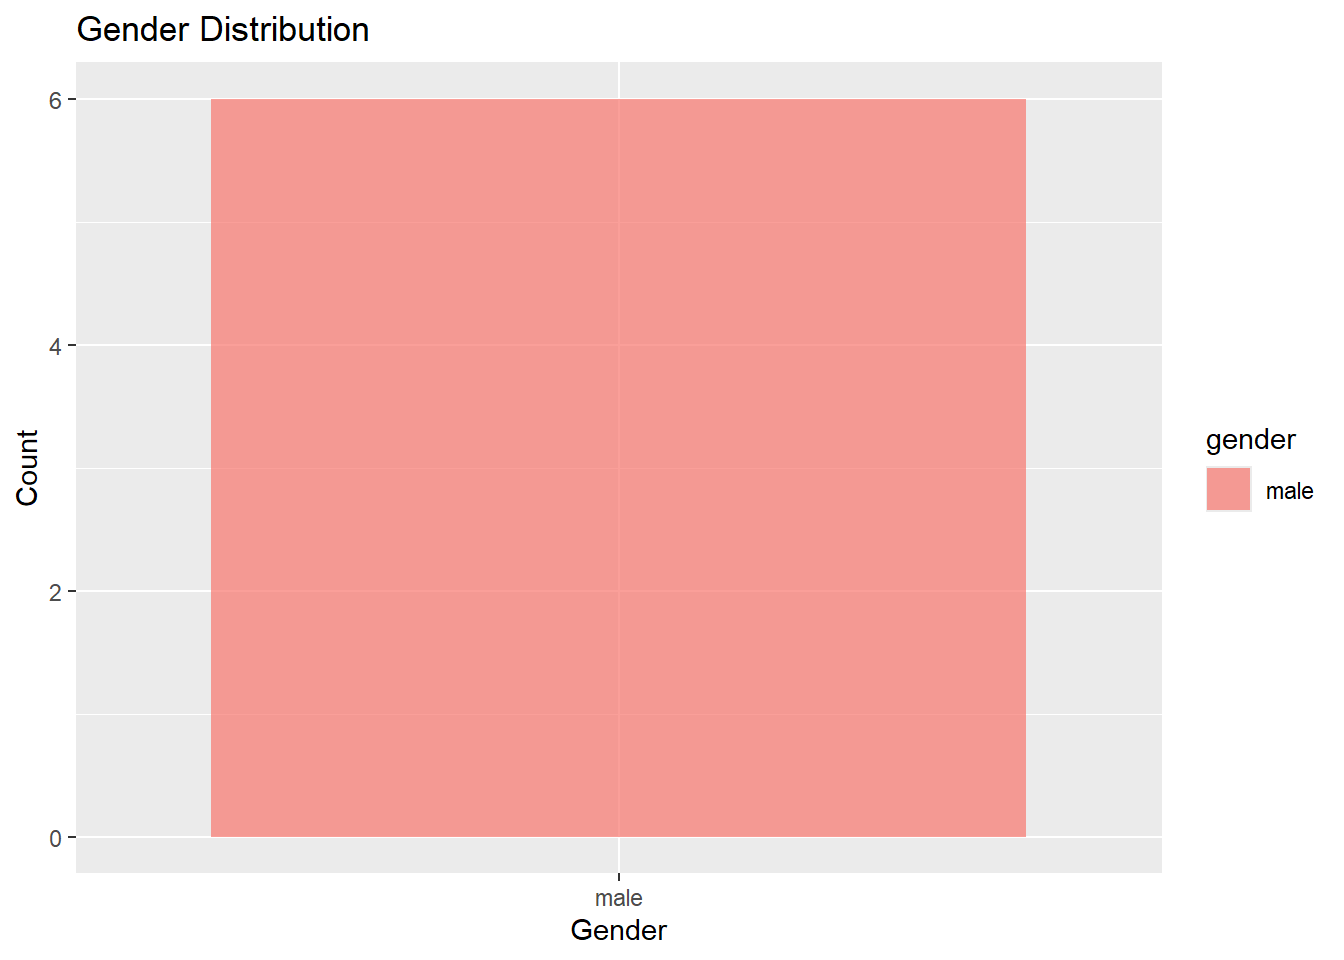
\includegraphics{Survey-Data-Analysis-of-Farmers-in-Jalgaon-District_files/figure-latex/unnamed-chunk-9-1.pdf}
\includegraphics{Survey-Data-Analysis-of-Farmers-in-Jalgaon-District_files/figure-latex/unnamed-chunk-9-2.pdf}
\includegraphics{Survey-Data-Analysis-of-Farmers-in-Jalgaon-District_files/figure-latex/unnamed-chunk-9-3.pdf}

\begin{verbatim}
## [1] "Missing Data Count per Variable:"
\end{verbatim}

\begin{verbatim}
##                                    farmer_id 
##                                           55 
##                                 farmers_name 
##                                            0 
##                                      village 
##                                            0 
##                                       taluka 
##                                            0 
##                                          age 
##                                            0 
##                                       gender 
##                                            0 
##                               marital_status 
##                                            0 
##                                    education 
##                                            0 
##                                     religion 
##                                            0 
##                                        caste 
##                                            0 
##                                     subcaste 
##                                            0 
##                                mother_tongue 
##                                            0 
##                                  family_type 
##                                            0 
##                               head_of_family 
##                                            0 
##                         relation_with_farmer 
##                                            0 
##                         total_family_members 
##                                            0 
##                               income_sources 
##                                            0 
##                   income_sources_agriculture 
##                                            0 
##                        income_sources_labour 
##                                            0 
##                           income_sources_job 
##                                          146 
##                      income_sources_business 
##                                            0 
##                    income_sources_privatejob 
##                                            0 
##                income_sources_government_job 
##                                            0 
##                       income_sources_pension 
##                                            0 
##                         income_sources_other 
##                                            0 
##                                  otherincome 
##                                          302 
##                         traditional_business 
##                                            0 
##                                annual_income 
##                                            0 
##                                   bpl_status 
##                                            0 
##                                  ration_card 
##                                            0 
##                                farmers_group 
##                                           62 
##                                     sh_group 
##                                           61 
##                                    land_type 
##                                            0 
##                               irrigated_land 
##                                            0 
##                                     dry_land 
##                                            0 
##                                   total_land 
##                                            0 
##                                 soil_testing 
##                                           67 
##                             soil_tested_year 
##                                          295 
##                                water_sources 
##                                            0 
##                           water_sources_none 
##                                            0 
##                          water_sources_river 
##                                            0 
##                           water_sources_well 
##                                            0 
##                          water_sources_canal 
##                                            0 
##                       water_sources_borewell 
##                                            0 
##                      water_sources_farm_pond 
##                                            0 
##                      water_sources_reservoir 
##                                            0 
##                            water_sources_dam 
##                                            0 
##                 water_sources_neighbor_water 
##                                            0 
##                                       cotton 
##                                           49 
##                                        maize 
##                                          189 
##                                        jowar 
##                                          237 
##                                        bajra 
##                                          246 
##                                       pulses 
##                                          246 
##                                      soybean 
##                                          250 
##                                        wheat 
##                                          226 
##                                         gram 
##                                          222 
##                                      sorghum 
##                                          250 
##                                       maize2 
##                                          221 
##                                    groundnut 
##                                          259 
##                                        melon 
##                                          258 
##                                       sesame 
##                                          260 
##                                       banana 
##                                          255 
##                                  pomegranate 
##                                          261 
##                                       citrus 
##                                          260 
##                                   vegetables 
##                                          260 
##                                  other_crops 
##                                            0 
##                                         x001 
##                                           39 
##                                 text_qi3tf85 
##                                          284 
##                                 text_pu6bd80 
##                                          122 
##                                     bullocks 
##                                            0 
##                                          cow 
##                                            0 
##                                      buffalo 
##                                            0 
##                                         goat 
##                                            0 
##                                        sheep 
##                                            0 
##                                      poultry 
##                                            0 
##                                 text_cu6dv88 
##                                          242 
##                                      sprayer 
##                                            0 
##                                        motor 
##                                            0 
##                                     thresher 
##                                            0 
##                                      tractor 
##                                            0 
##                                    other_001 
##                                          218 
##                                  farm_income 
##                                            0 
##                              monthly_expense 
##                                            0 
##                           select_one_ld4vw19 
##                                           65 
##                           secondary_business 
##                                            0 
##                                business_type 
##                                            0 
##                          business_type_labor 
##                                            0 
##                          business_type_dairy 
##                                            0 
##                        business_type_poultry 
##                                            0 
##                            business_type_job 
##                                            0 
##                        business_type_cottage 
##                                            0 
##                   business_type_goat_farming 
##                                            0 
##                          business_type_other 
##                                            0 
##                                 text_yx7ko73 
##                                          229 
##                                 text_cu8jm42 
##                                          122 
##                                  loan_status 
##                                            0 
##                                  loan_amount 
##                                           36 
##                                 loan_purpose 
##                                           36 
##              loan_purpose_agriculture_inputs 
##                                           36 
##           loan_purpose_agriculture_machinery 
##                                           36 
##                       loan_purpose_crop_loss 
##                                           36 
##                  loan_purpose_debt_repayment 
##                                           36 
##                 loan_purpose_household_needs 
##                                           36 
##          loan_purpose_supplementary_business 
##                                           36 
##                           loan_purpose_other 
##                                           36 
##                            loan_other_reason 
##                                          297 
##                                  loan_source 
##                                           36 
##                             loan_source_bank 
##                                           36 
##                   loan_source_private_lender 
##                                           36 
##                      loan_source_cooperative 
##                                           36 
##                loan_source_relatives_friends 
##                                           36 
##                  loan_source_self_help_group 
##                                           36 
##                     loan_source_microfinance 
##                                           36 
##                            loan_source_other 
##                                           36 
##                                    bank_name 
##                                          159 
##                                bank_name_001 
##                                          299 
##                                loan_duration 
##                                           36 
##                                 overdue_loan 
##                                           36 
##                             overdue_duration 
##                                           36 
##                              subsidized_loan 
##                                           36 
##                      health_conditions_other 
##                                          235 
##                             low_market_price 
##                                            0 
##                               climate_change 
##                                            0 
##                           irrigation_problem 
##                                            0 
##                         high_fertilizer_cost 
##                                            0 
##                         lack_of_govt_support 
##                                            0 
##                                  labour_cost 
##                                            0 
##                       middleman_exploitation 
##                                            0 
##                         high_production_cost 
##                                            0 
##                             inflation_stress 
##                                            0 
##                     lack_of_processing_units 
##                                            0 
##                            electricity_issue 
##                                            0 
##                             no_minimum_price 
##                                            0 
##                                 no_farm_loan 
##                                            0 
##                                 pest_disease 
##                                            0 
##                              disaster_damage 
##                                            0 
##                              no_compensation 
##                                            0 
##                      storage_marketing_issue 
##                                            0 
##                       lack_of_family_support 
##                                            0 
##                              tech_resistance 
##                                            0 
##                                  aadhar_card 
##                                            0 
##                                     voter_id 
##                                            0 
##                         ayushman_bharat_card 
##                                            0 
##                                pm_kisan_card 
##                                            0 
##                                     job_card 
##                                           56 
##                            pml_ife_insurance 
##                                           57 
##                               caste_validity 
##                                            0 
##                           caste_validity_001 
##                                            0 
##                       caste_validity_001_001 
##                                            0 
##                            caste_certificate 
##                                            0 
##                  age_nationality_certificate 
##                                            0 
##                                     pan_card 
##                                            0 
##                                 bank_account 
##                                            0 
##                              ration_card_001 
##                                            0 
##                              driving_license 
##                                            0 
##                                     pm_kisan 
##                                            0 
##                             pm_kisan_mandhan 
##                                            0 
##                         pm_kisan_mandhan_001 
##                                            0 
##                     pm_kisan_mandhan_001_001 
##                                            0 
##                 pm_kisan_mandhan_001_001_001 
##                                            0 
##                                        pmksy 
##                                            0 
##                                        pmfby 
##                                            0 
##                                 kisan_credit 
##                                            0 
##                                  loan_waiver 
##                                            0 
##                              organic_farming 
##                                            0 
##                          organic_farming_001 
##                                            0 
##                                  aif_funding 
##                                            0 
##                                    agri_tech 
##                                            0 
##                                    farm_pond 
##                                            0 
##                               community_pond 
##                                            0 
##                               tractor_scheme 
##                                            0 
##                           accident_insurance 
##                                            0 
##                              farmer_training 
##                                            0 
##                              tree_plantation 
##                                            0 
##                                   solar_pump 
##                                            0 
##                           water_conservation 
##                                            0 
##                              market_facility 
##                                            0 
##                                     agri_dev 
##                                            0 
##                              rupee_insurance 
##                                            0 
##                                         atma 
##                                            0 
##                                 difficulties 
##                                           57 
##                               difficulties_1 
##                                           57 
##                               difficulties_2 
##                                           57 
##                               difficulties_3 
##                                           57 
##                               difficulties_4 
##                                           57 
##                               difficulties_5 
##                                           57 
##                           other_difficulties 
##                                          276 
##                          scheme_info_sources 
##                                            0 
## scheme_info_sources_local_agriculture_office 
##                                            0 
##              scheme_info_sources_cooperative 
##                                            0 
##                 scheme_info_sources_tv_radio 
##                                            0 
##            scheme_info_sources_internet_apps 
##                                            0 
##                      scheme_info_sources_ngo 
##                                            0 
##                        scheme_info_sources_2 
##                                            0 
##                           other_info_sources 
##                                          290 
##                          scheme_improvements 
##                                            0 
##       scheme_improvements_more_info_training 
##                                            0 
##       scheme_improvements_simplified_process 
##                                            0 
##       scheme_improvements_local_help_centers 
##                                            0 
##                    scheme_improvements_other 
##                                            0 
##                           other_improvements 
##                                          303 
##                              family_problems 
##                                            0 
##                               suicide_causes 
##                                            0 
##                           suicide_prevention 
##                                            0 
##                             govt_initiatives 
##                                            0 
##                             farming_training 
##                                            0 
##                             alternate_income 
##                                            0 
##                               informant_name 
##                                            0 
##                             informant_mobile 
##                                            0 
##                                surveyor_name 
##                                            0 
##                                 depression_1 
##                                            0 
##                                 depression_2 
##                                            0 
##                                 depression_3 
##                                            0 
##                                 depression_4 
##                                            0 
##                                 depression_5 
##                                            0 
##                                    anxiety_1 
##                                            0 
##                                    anxiety_2 
##                                            0 
##                                    anxiety_3 
##                                            0 
##                                    anxiety_4 
##                                            0 
##                             social_support_1 
##                                            0 
##                             social_support_2 
##                                            0 
##                             social_support_3 
##                                            0 
##                             social_support_4 
##                                            0 
##                          suicidal_ideation_1 
##                                            0 
##                          suicidal_ideation_2 
##                                            0 
##                          suicidal_ideation_3 
##                                            0 
##                           financial_stress_1 
##                                            0 
##                           financial_stress_2 
##                                            0 
##                           financial_stress_3 
##                                            0 
##                           financial_stress_4 
##                                            0 
##                                     coping_1 
##                                            0 
##                                     coping_2 
##                                            0 
##                                     coping_3 
##                                            0 
##                                     coping_4 
##                                            0 
##                          life_satisfaction_1 
##                                            0 
##                          life_satisfaction_2 
##                                            0 
##                          life_satisfaction_3 
##                                            0 
##                          life_satisfaction_4 
##                                            0 
##                             member_depressed 
##                                            0 
##                               mental_support 
##                                            0 
##                                 medical_need 
##                                            0 
##                       govt_schemes_awareness 
##                                            0 
##                        positive_mental_state 
##                                            0 
##                         social_participation 
##                                            0 
##                          govt_support_needed 
##                                            0 
##                         education_continuity 
##                                            0 
##                                 housing_type 
##                                            0 
##                            housing_condition 
##                                            0 
##                      additional_observations 
##                                            0 
##     point_and_shoot_use_mera_to_take_a_photo 
##                                            1 
## point_and_shoot_use_mera_to_take_a_photo_url 
##                                            1 
##                                         x003 
##                                          249 
##                                 text_ye0iz81 
##                                          303 
##                                         x005 
##                                          303 
##                               life_insurance 
##                                          303 
##                                         x006 
##                                          251 
##                               agri_insurance 
##                                          303 
##                                         x007 
##                                          249 
##                             cropping_pattern 
##                                          303 
##                                            x 
##                                          252 
##                                 crops_kharif 
##                                          303 
##                           crops_kharif_jowar 
##                                          303 
##                           crops_kharif_bajra 
##                                          303 
##                           crops_kharif_maize 
##                                          303 
##                      crops_kharif_urad_moong 
##                                          303 
##                         crops_kharif_soybean 
##                                          303 
##                               crops_kharif_2 
##                                          303 
##                                         x008 
##                                          302 
##                                   crops_rabi 
##                                          303 
##                             crops_rabi_wheat 
##                                          303 
##                              crops_rabi_gram 
##                                          303 
##                        crops_rabi_jowar_late 
##                                          303 
##                                 crops_rabi_2 
##                                          303 
##                                 crops_summer 
##                                          303 
##                           crops_summer_maize 
##                                          303 
##                       crops_summer_sugarcane 
##                                          303 
##                       crops_summer_groundnut 
##                                          303 
##                  crops_summer_cucumber_melon 
##                                          303 
##                               crops_summer_2 
##                                          303 
##                           crops_horticulture 
##                                          303 
##                    crops_horticulture_banana 
##                                          303 
##               crops_horticulture_pomegranate 
##                                          303 
##                    crops_horticulture_citrus 
##                                          303 
##                         crops_horticulture_2 
##                                          303 
##                                        other 
##                                          303 
##                                         x009 
##                                          299 
##                                         x010 
##                                          259 
##                                 text_lo1xd85 
##                                          303 
##                                         x011 
##                                          274 
##                            health_conditions 
##                                          303 
##              health_conditions_heart_disease 
##                                          303 
##                   health_conditions_diabetes 
##                                          303 
##        health_conditions_respiratory_disease 
##                                          303 
##              health_conditions_mental_stress 
##                                          303 
##                    health_conditions_other_2 
##                                          303 
##                                         x012 
##                                          250 
##                                         x013 
##                                          278 
##                                         x014 
##                                          258 
##                                         x015 
##                                          303 
##                         other_farming_issues 
##                                          303 
##                                   job_card_2 
##                                          303 
##                                         x017 
##                                          249 
##                            balasaheb_project 
##                                          303 
##                                         x018 
##                                          250 
##                           ahilyadevi_nursery 
##                                          303 
##                                other_schemes 
##                                          303 
##                                         x002 
##                                          249 
##                                       x002_1 
##                                          249 
##                                       x002_2 
##                                          249 
##                                       x002_3 
##                                          249 
##                                       x002_4 
##                                          249 
##                                       x002_5 
##                                          249 
##                                           id 
##                                            0 
##                                         uuid 
##                                            0 
##                              submission_time 
##                                            0 
##                            validation_status 
##                                          290 
##                                        notes 
##                                          303 
##                                       status 
##                                            0 
##                                 submitted_by 
##                                          303 
##                                      version 
##                                            0 
##                                         tags 
##                                          303 
##                                        index 
##                                            0
\end{verbatim}

\includegraphics{Survey-Data-Analysis-of-Farmers-in-Jalgaon-District_files/figure-latex/unnamed-chunk-9-4.pdf}

\begin{verbatim}
## [1] "Cross-Tabulation: Gender, Marital Status, and BPL Status"
\end{verbatim}

\begin{verbatim}
## , ,  = no
## 
##         
##            _ divorced married unmarried
##   female   1        0       2         0
##   male     1        1     117        14
## 
## , ,  = yes
## 
##         
##            _ divorced married unmarried
##   female   0        0       2         0
##   male     3        2     140        20
\end{verbatim}

\includegraphics{Survey-Data-Analysis-of-Farmers-in-Jalgaon-District_files/figure-latex/unnamed-chunk-9-5.pdf}
\includegraphics{Survey-Data-Analysis-of-Farmers-in-Jalgaon-District_files/figure-latex/unnamed-chunk-9-6.pdf}

\end{document}
